\documentclass[11pt, a4paper, notitlepage]{report}

\usepackage{amsmath, amssymb, amsthm}
\usepackage{geometry}
\geometry{margin=1in}
\usepackage{microtype}           % microtypography: prevents most overfull hboxes
\usepackage{hyperref}
\hypersetup{colorlinks=true, linkcolor=blue!60!black, urlcolor=blue!60!black,
            breaklinks=true}     % allow URLs to break across lines
\usepackage{xurl}                % aggressive URL line-breaking (load AFTER hyperref)
\usepackage{enumitem}
\usepackage{algorithm}
\usepackage{algpseudocode}
\usepackage{listings}
\usepackage{xcolor}
\usepackage[most]{tcolorbox}
\tcbuselibrary{theorems}
\usepackage{titlesec}
\usepackage{booktabs}
\usepackage{array}
\usepackage{tabularx}           % auto-width columns that wrap text
\usepackage{tikz}
\usetikzlibrary{arrows.meta, shapes.geometric, positioning, fit, calc}
\setcounter{secnumdepth}{3}

% ── Overflow prevention ───────────────────────────────────────────────────────
\sloppy
\setlength{\emergencystretch}{3em}

% ── Highlight boxes ───────────────────────────────────────────────────────────
\newtcolorbox{keyresult}[1][]{
  enhanced, colback=blue!5!white, colframe=blue!60!black,
  fonttitle=\bfseries, title={Key Result}, #1
}
\newtcolorbox{examtip}[1][]{
  enhanced, colback=green!5!white, colframe=green!50!black,
  fonttitle=\bfseries, title={Exam Tip}, #1
}
\newtcolorbox{warning}[1][]{
  enhanced, colback=red!5!white, colframe=red!60!black,
  fonttitle=\bfseries, title={Warning}, #1
}

% ── Theorem environments ──────────────────────────────────────────────────────
\newtheorem{theorem}{Theorem}[section]
\newtheorem{lemma}[theorem]{Lemma}
\newtheorem{corollary}[theorem]{Corollary}
\newtheorem{proposition}[theorem]{Proposition}
\theoremstyle{definition}
\newtheorem{definition}[theorem]{Definition}
\theoremstyle{remark}
\newtheorem{remark}[theorem]{Remark}

% ── Example environment (amsthm) ─────────────────────────────────────────────
% Plain amsthm theorem style. Usage:
%   \begin{example}[Title]   -> "Example 1.3 (Title)"
%   \begin{example}          -> "Example 1.4"
%   \label{ex:...} / \ref{ex:...} for cross-references (place \label inside)
\theoremstyle{definition}
\newtheorem{example}[theorem]{Example}

% ── Code listings ─────────────────────────────────────────────────────────────
\definecolor{codebg}{RGB}{245,247,250}
\definecolor{codeborder}{RGB}{180,190,210}
\definecolor{codekw}{RGB}{0,80,180}
\definecolor{codecomment}{RGB}{100,110,130}
\definecolor{codestring}{RGB}{160,40,40}

\lstset{
  basicstyle=\ttfamily\footnotesize,
  keywordstyle=\color{codekw}\bfseries,
  commentstyle=\color{codecomment}\itshape,
  stringstyle=\color{codestring},
  breaklines=true,
  breakatwhitespace=false,
  breakautoindent=true,
  postbreak=\mbox{\textcolor{codecomment}{$\hookrightarrow$}\space},
  columns=flexible,
  backgroundcolor=\color{codebg},
  frame=single,
  frameround=ffff,
  framesep=5pt,
  rulecolor=\color{codeborder},
  aboveskip=6pt,
  belowskip=6pt,
  xleftmargin=6pt,
  xrightmargin=6pt,
  numbers=left,
  numberstyle=\ttfamily\tiny\color{codecomment},
  numbersep=8pt,
  showstringspaces=false,
  tabsize=4
}

% Suppress "Listing N:" caption label
\renewcommand\lstlistingname{}

% ── Suppress "Listing N:" caption prefix ─────────────────────────────────────
\renewcommand\lstlistingname{}
% \renewcommand\thelstlisting{}  % removed: command undefined without caption pkg

% ── Suppress forced page break in \tableofcontents ────────────────────────────
\makeatletter
\renewcommand\tableofcontents{%
  \section*{\contentsname}%
  \@starttoc{toc}%
}
\makeatother

% ── Chapter title formatting ──────────────────────────────────────────────────
\titleformat{\chapter}[display]
  {\normalfont\LARGE\bfseries}
  {\chaptertitlename\ \thechapter}{12pt}{\Huge}
\titlespacing*{\chapter}{0pt}{20pt}{30pt}

% ── Title block (filled in by generation script) ──────────────────────────────
% \title{\textbf{<Course Code>: <Course Name>}\\[0.5em]
%        \large <Subtitle>}
% \author{}
% \date{}

\title{\textbf{SC1007: Data Structures and Algorithms}\\[0.5em]
       \large Lecture Notes}
\author{}
\date{}

\begin{document}
\maketitle
\tableofcontents
\newpage

\chapter{Introduction \& Memory Management in Python}
\label{ch:memory-management}

\section{Introduction to Memory Management}
\label{sec:intro-mm}

Memory management refers to the critical process of allocating, deallocating, and coordinating
computer memory effectively. The primary objective is to ensure that all processes execute
smoothly and efficiently utilise system resources. In Python, this is achieved through a
combination of dynamic memory allocation, automatic garbage collection, and reference counting
mechanisms.

\begin{definition}[Memory Management]
\label{def:memory-management}
Memory management is the process of controlling and coordinating a program's access to memory,
encompassing allocation of memory to running processes, tracking which parts of memory are in
use, and reclaiming memory when it is no longer needed.
\end{definition}

Python's memory management subsystem provides several key features:
\begin{itemize}
  \item \textbf{Automatic Memory Management:} Python handles memory allocation and
        deallocation without developer intervention.
  \item \textbf{Memory Pooling:} Previously allocated memory blocks are reused to
        reduce overhead.
  \item \textbf{Memory Fragmentation Prevention:} Efficient organisation of memory
        blocks reduces wasted gaps.
\end{itemize}

The benefits of Python's approach include prevention of memory leaks, optimised memory usage,
reduced development complexity, and improved application performance. Poor memory management
leads to program crashes and degraded performance.

\begin{keyresult}[title={Core Memory Management Mechanisms}]
Python employs five main mechanisms working in concert:
\begin{enumerate}
  \item Reference Counting
  \item Garbage Collection
  \item Memory Pooling
  \item Memory Interning
  \item Manual Memory Management
\end{enumerate}
\end{keyresult}

% ─────────────────────────────────────────────────────────────────────────────
\section{Names, References, and Objects}
\label{sec:names-refs-objs}

Understanding Python's memory model requires distinguishing three distinct concepts:

\begin{definition}[Name (Variable)]
A name is a label or identifier that \emph{points to} an object in memory. A Python variable
does not directly hold a value; it holds a reference to where the value lives in the heap.
\end{definition}

\begin{definition}[Reference]
A reference is the link between a name and an object. It stores the memory address of the
object, allowing Python to locate and access it without embedding the value in the variable
itself.
\end{definition}

\begin{definition}[Object]
An object is the actual entity stored in memory --- an integer, string, list, or user-defined
instance. Every object has a unique memory address, a type, a value, and a reference count.
\end{definition}

\begin{example}[Name, Reference, and Object]
When we write \texttt{x = 42}, Python creates an integer object \texttt{42} in the heap, then
binds the name \texttt{x} to that object via a reference. Calling \texttt{id(x)} returns the
memory address of the object.
\begin{lstlisting}[language=Python]
x = 42
print(id(x))   # e.g., 140712834927920
\end{lstlisting}
The name \texttt{x} lives on the stack; the integer object \texttt{42} lives on the heap.
\end{example}

% ─────────────────────────────────────────────────────────────────────────────
\section{Python Memory Layout}
\label{sec:memory-layout}

Python programs use four distinct memory regions, each with a specific role.

\begin{definition}[Code Segment]
Stores the compiled Python bytecode and program instructions. This region is read-only during
execution.
\end{definition}

\begin{definition}[Static/Global Segment]
Stores global variables and static data that persist throughout the entire program's
execution (e.g., module-level variables).
\end{definition}

\begin{definition}[Stack]
Used for function call frames, local variables, and references. Each function call pushes a
new frame; when the function returns, its frame is popped and all local names are removed.
\end{definition}

\begin{definition}[Heap (Dynamic Memory)]
Used to store dynamically allocated objects: lists, dictionaries, class instances, and all
other runtime objects. Managed automatically by Python's garbage collector.
\end{definition}

\begin{keyresult}[title={Memory Layout Summary}]
\begin{center}
\begin{tabularx}{\linewidth}{lX}
\toprule
\textbf{Segment} & \textbf{Contents} \\
\midrule
Code & Python bytecode, program instructions \\
Static/Global & Global variables, static data (live for program lifetime) \\
Stack & Function call frames, local variables, name-to-address bindings \\
Heap & All objects (integers, lists, dicts, user-defined); GC-managed \\
\bottomrule
\end{tabularx}
\end{center}
\end{keyresult}

% ─────────────────────────────────────────────────────────────────────────────
\section{Immutable vs.\ Mutable Object Memory Characteristics}
\label{sec:mut-immut}

\subsection{Immutable Objects (Integers and Strings)}
\label{subsec:immutable}

Integers and strings are \emph{immutable}: their value cannot be changed after creation.
Any apparent modification creates an entirely new object in the heap.

\begin{example}[Integer Reassignment]
When \texttt{y = x} is executed, both names point to the same object. After \texttt{x += 1},
\texttt{x} is rebound to a newly created integer object; \texttt{y} still points to the
original.
\begin{lstlisting}[language=Python]
x = 42
y = x          # x and y both reference the same object (0x1234)
x += 1         # creates new int 43 at a new address; y unchanged
# After: x -> 0x5678 (value 43), y -> 0x1234 (value 42)
\end{lstlisting}
\end{example}

\begin{example}[String Immutability and Object Reuse]
Because strings are immutable, Python can safely let two names reference the same string
object (this is called \emph{interning}). Reassigning one name creates a new object and
leaves the other name unaffected.
\begin{lstlisting}[language=Python]
s1 = "hello"
s2 = "hello"   # s1 and s2 share the same heap object (refcount: 2)
s1 = "hello!"  # new object created for s1; s2 still points to "hello"
\end{lstlisting}
\end{example}

\begin{warning}[title={Warning: Immutability Does Not Mean Unrebindable}]
Immutability means the \emph{object's value} cannot change. The \emph{name} can always be
rebound to a different object. \texttt{x += 1} for an integer does \emph{not} modify the
integer in place; it creates a new integer and rebinds \texttt{x}.
\end{warning}

\subsection{Mutable Objects (Lists, Dicts, Sets)}
\label{subsec:mutable}

Mutable objects can be modified in place. When two names reference the same mutable object,
a mutation through either name is visible through the other.

\begin{example}[Shared Mutable List]
After \texttt{list2 = list1}, both names point to the same \texttt{PyList} object. Appending
via \texttt{list1} changes the object that \texttt{list2} also sees.
\begin{lstlisting}[language=Python]
list1 = [1, 2, 3]   # PyList at 0x1234; refcount: 1
list2 = list1        # refcount: 2; list1 and list2 -> 0x1234
list1.append(4)      # modifies the object in place; list2 now also [1,2,3,4]
\end{lstlisting}
\end{example}

\begin{examtip}[title={Exam Tip: \texttt{is} vs.\ \texttt{==} for Mutable Objects}]
Use \texttt{==} to compare \emph{values}. Use \texttt{is} to check whether two names point to
the \emph{same object} (same \texttt{id()}). For mutable objects, \texttt{a is b} is
\texttt{True} only when both names reference the same heap location, not merely equal
contents.
\end{examtip}

% ─────────────────────────────────────────────────────────────────────────────
\section{Reference Counting}
\label{sec:refcount}

Reference counting is Python's \emph{primary} memory management mechanism. Every object on the
heap maintains an integer counter tracking the number of names (or containers) currently
pointing to it. When the counter drops to zero the object is immediately deallocated.

\begin{definition}[Reference Count]
The reference count of an object is the number of active references pointing to it. It
increments when a new name is bound to the object or the object is stored in a container, and
decrements when a name is deleted or rebound.
\end{definition}

\subsection{Advantages of Reference Counting}
\label{subsec:refcount-adv}

\begin{itemize}
  \item \textbf{Predictable Performance:} Memory is freed immediately when no longer needed,
        avoiding unpredictable pause times.
  \item \textbf{Deterministic Resource Management:} Resources (e.g., file handles) are
        released promptly, making reference counting well-suited to real-time systems.
  \item \textbf{Simplicity:} The mechanism is straightforward to reason about and transparent
        to developers.
  \item \textbf{Memory Efficiency:} Reduced memory footprint and better cache utilisation
        because dead objects are reclaimed instantly.
\end{itemize}

\subsection{Reference Counting in Practice}
\label{subsec:refcount-example}

The \texttt{sys.getrefcount()} function returns the reference count of an object. Note that
calling the function itself creates a temporary reference, so the reported count is one higher
than the actual live count; subtract 1 to get the true value.

\begin{example}[Incrementing and Decrementing the Reference Count]
\leavevmode
\begin{lstlisting}[language=Python]
import sys

x = [1, 2, 3]
print(sys.getrefcount(x) - 1)  # 1  (only x references the list)

y = x
print(sys.getrefcount(x) - 1)  # 2  (x and y both reference it)

z = x
print(sys.getrefcount(z) - 1)  # 3  (x, y, z)

del x   # refcount -> 2
del y   # refcount -> 1
del z   # refcount -> 0  => object eligible for garbage collection
\end{lstlisting}
When the final reference is removed (\texttt{del z}), the list's reference count reaches zero
and Python's allocator immediately reclaims the heap memory.
\end{example}

\subsection{Disadvantages of Reference Counting}
\label{subsec:refcount-disadv}

\begin{itemize}
  \item \textbf{Overhead Costs:} Every assignment and deletion must update the counter,
        consuming CPU cycles and extra memory.
  \item \textbf{Circular References:} If two objects reference each other, neither count ever
        reaches zero even when both become unreachable from the program. This requires a
        supplementary cyclic garbage collector.
  \item \textbf{Threading Complications:} Reference count updates must be atomic to be
        thread-safe. Python's Global Interpreter Lock (GIL) ensures this but limits
        multi-threaded parallelism.
\end{itemize}

\subsection{Circular References}
\label{subsec:circular-refs}

A circular reference occurs when two or more objects reference each other, forming a cycle.
Because each object in the cycle holds a non-zero count (due to the internal references), the
cycle persists in memory even after all external names are deleted.

\begin{example}[Circular Reference Between Two Lists]
\leavevmode
\begin{lstlisting}[language=Python]
list1 = []
list2 = []
list1.append(list2)  # list1 contains a reference to list2
list2.append(list1)  # list2 contains a reference to list1

del list1  # still referenced by list2[0]; refcount does not reach 0
del list2  # still referenced by list1[0]; refcount does not reach 0
# Both objects are unreachable but NOT yet collected by reference counting.
# The cyclic garbage collector detects the cycle and frees both.
\end{lstlisting}
\end{example}

\begin{warning}[title={Warning: Circular References Cause Memory Leaks Without GC}]
Pure reference counting cannot reclaim circular garbage. Python supplements reference counting
with a \emph{cyclic garbage collector} (the \texttt{gc} module) specifically to handle cycles.
Always be mindful of circular structures in long-running programs.
\end{warning}

\subsection{Threading and the Mutex Solution}
\label{subsec:mutex}

In a multi-threaded environment, two threads could simultaneously modify the same reference
count, producing an incorrect value (a \emph{race condition}). Python's solution at the
interpreter level is the GIL. At the application level, mutual-exclusion locks (mutexes) ensure
that only one thread accesses a shared resource at a time: Thread 1 acquires the lock,
completes its read-modify-write, then releases the lock before Thread 2 may proceed.

% ─────────────────────────────────────────────────────────────────────────────
\section{Garbage Collection}
\label{sec:gc}

Python's cyclic garbage collector (the \texttt{gc} module) supplements reference counting to
handle objects involved in cycles.

\begin{definition}[Garbage Collection]
Garbage collection is the automatic process of detecting objects that are no longer reachable
from the program and reclaiming the memory they occupy.
\end{definition}

\subsection{Generational Collection}
\label{subsec:generations}

Python's garbage collector uses a \emph{three-generation} model based on the empirical
observation that most objects die young (\emph{generational hypothesis}):

\begin{itemize}
  \item \textbf{Generation 0 (Young):} Newly created objects. Collected most frequently
        (triggered after every 700 new object allocations). Objects that survive are promoted
        to Generation 1.
  \item \textbf{Generation 1 (Middle-Aged):} Objects that survived at least one
        Generation~0 sweep. Collected after every 10 Generation~0 collections. Survivors are
        promoted to Generation~2.
  \item \textbf{Generation 2 (Old):} Long-lived objects (e.g., global configuration
        dictionaries). Collected least frequently --- after every 10 Generation~1 collections.
\end{itemize}

\begin{keyresult}[title={Key Result: Generational GC Thresholds (Default)}]
\begin{center}
\begin{tabularx}{\linewidth}{@{}l X l@{}}
\toprule
\textbf{Generation} & \textbf{Typical Contents} & \textbf{Collection Trigger} \\
\midrule
0 (Young) & Temporary loop vars, intermediate results & Every $\sim$700 allocations \\
1 (Middle) & Session-scoped objects (e.g., a shopping cart) & After 10 Gen-0 sweeps \\
2 (Old) & Module-level singletons, global config & After 10 Gen-1 sweeps \\
\bottomrule
\end{tabularx}
\end{center}
\end{keyresult}

\subsection{Advantages and Disadvantages}
\label{subsec:gc-tradeoffs}

\begin{itemize}
  \item \textbf{Advantages:} Handles circular references that reference counting alone cannot
        collect; automatic with no developer effort; safer memory management.
  \item \textbf{Disadvantages:} Collection pauses introduce non-deterministic latency;
        higher memory usage (objects linger until the next sweep); resource-intensive for
        large object graphs.
\end{itemize}

\subsection{Forcing Garbage Collection}
\label{subsec:force-gc}

Developers can take manual control of the garbage collector via the \texttt{gc} module.

\begin{example}[Manual Garbage Collection to Clear Circular References]
The following pattern disables automatic collection during a critical section, then forces a
collection sweep to resolve a known circular reference.
\begin{lstlisting}[language=Python]
import gc

gc.disable()   # suppress automatic GC during sensitive operations

list1 = [1, 2, 3]
list2 = [4, 5, 6]
list1.append(list2)   # circular reference
list2.append(list1)

del list1   # refcount still non-zero due to cycle
del list2

gc.collect()   # cyclic GC detects and frees both objects
gc.enable()    # restore automatic GC
\end{lstlisting}
After \texttt{gc.collect()}, both list objects are freed and the heap memory is reclaimed.
\end{example}

% ─────────────────────────────────────────────────────────────────────────────
\section{Memory Pooling}
\label{sec:pooling}

\begin{definition}[Memory Pooling]
Memory pooling is an optimisation technique in which Python pre-allocates fixed-size blocks of
memory and reuses them for small, frequently created objects, avoiding the overhead of repeated
system-level allocation and deallocation calls.
\end{definition}

Key characteristics:
\begin{itemize}
  \item \textbf{Pre-allocation:} Blocks are reserved ahead of time to reduce allocation cost.
  \item \textbf{Fixed-size Pools:} Separate pools are maintained for different object sizes.
  \item \textbf{Efficient Reuse:} When a pooled object is deleted its slot is returned to the
        pool rather than released to the OS.
  \item \textbf{Automatic:} Python manages pooling internally via its \emph{pymalloc}
        allocator; no developer action is required.
\end{itemize}

\begin{example}[Small Integer and String Pooling]
Small integers (typically $-5$ to $256$) and short identifier-like strings are pooled, so
two names holding the same value share the same heap object:
\begin{lstlisting}[language=Python]
a = 100
b = 100
print(a is b)      # True  -- same object from the integer pool

str1 = "hello"
str2 = "hello"
print(str1 is str2)  # True  -- same object from the string pool
\end{lstlisting}
\end{example}

\begin{warning}[title={Warning: Pool Sharing is an Implementation Detail}]
Integer pooling for values outside $[-5, 256]$ and string interning behaviour are
\emph{CPython} implementation details that may differ between Python implementations (e.g.,
PyPy, Jython). Never rely on \texttt{is} for value equality of integers or strings in
production code; always use \texttt{==}.
\end{warning}

% ─────────────────────────────────────────────────────────────────────────────
\section{Memory Interning}
\label{sec:interning}

\begin{definition}[Memory Interning]
Interning is an optimisation in which Python caches a single canonical copy of an immutable
object (typically a string or small integer) and reuses it for all bindings with the same
value, saving memory and enabling fast identity comparisons.
\end{definition}

\begin{itemize}
  \item Short strings and small integers are \emph{automatically} interned.
  \item Interned objects with identical values share the same memory address, so \texttt{is}
        returns \texttt{True}.
  \item Longer or dynamically constructed strings are \emph{not} automatically interned;
        \texttt{sys.intern()} enables manual interning.
\end{itemize}

\subsection{Automatic Interning}
\label{subsec:auto-intern}

\begin{example}[Short Strings Share an Address]
\leavevmode
\begin{lstlisting}[language=Python]
a = "hello"
b = "hello"
print(id(a) == id(b))  # True  -- same cached object
print(a is b)          # True

c = "hello world!"
d = "hello world!"
print(c is d)          # False -- longer string; not automatically interned
\end{lstlisting}
\end{example}

\subsection{Manual Interning with \texttt{sys.intern()}}
\label{subsec:manual-intern}

For longer strings that appear frequently (e.g., dictionary keys loaded from a large dataset),
manual interning can reduce memory usage and speed up comparisons.

\begin{example}[Manual Interning]
\leavevmode
\begin{lstlisting}[language=Python]
import sys

e = sys.intern("hello world!")
f = sys.intern("hello world!")
print(e is f)  # True -- sys.intern() stores one canonical copy
\end{lstlisting}
\end{example}

\begin{examtip}[title={Exam Tip: Interning Advantages and Limitations}]
\textbf{Advantage:} Faster equality checks using \texttt{is} (pointer comparison) instead of
\texttt{==} (character-by-character comparison). \textbf{Limitation:} Only effective for
immutable objects; manually interning mutable types has no effect.
\end{examtip}

% ─────────────────────────────────────────────────────────────────────────────
\section{Manual Memory Management}
\label{sec:manual-mm}

Although Python's automatic mechanisms handle most cases, developers occasionally need explicit
control, particularly for memory-intensive applications or resource-constrained systems.

\subsection{The \texttt{del} Keyword}
\label{subsec:del}

\texttt{del} explicitly removes a name-to-object binding from the current scope, decrementing
the object's reference count. If the count reaches zero, the object is immediately deallocated.

\begin{example}[Explicit Deletion with \texttt{del}]
\leavevmode
\begin{lstlisting}[language=Python]
x = 42
y = x                    # refcount of int-42 is now 2
list1 = [1, 2, 3, 4, 5]
list2 = list1            # refcount of the list is now 2

del x, y                 # refcount of int-42 drops to 0 -> freed
del list1, list2         # refcount of list drops to 0 -> freed
# Both objects are now eligible for garbage collection.
\end{lstlisting}
\end{example}

\begin{warning}[title={Warning: \texttt{del} Removes the Name, Not Necessarily the Object}]
\texttt{del x} only removes the binding \texttt{x}. If other names still reference the same
object its reference count does not reach zero and the object is \emph{not} freed. The object
is reclaimed only when \emph{all} references to it are removed.
\end{warning}

\subsection{Weak References}
\label{subsec:weakref}

A \emph{weak reference} points to an object without incrementing its reference count. This
allows the referenced object to be garbage collected when only weak references remain.

\begin{definition}[Weak Reference]
A weak reference is a reference that does not contribute to an object's reference count. When
the object is collected, accessing the weak reference returns \texttt{None}.
\end{definition}

\begin{example}[Using \texttt{weakref.ref()}]
\leavevmode
\begin{lstlisting}[language=Python]
import weakref
import sys

def my_function():
    return "Hello"

print(sys.getrefcount(my_function) - 1)  # 1 (normal ref count)

weak_ref = weakref.ref(my_function)
# refcount is STILL 1 -- weak reference does not increment it

print(weak_ref()())   # calls the function through the weak ref -> "Hello"

del my_function       # refcount drops to 0; object collected
print(weak_ref())     # None -- the object no longer exists
\end{lstlisting}
\end{example}

\begin{keyresult}[title={Key Result: Strong vs.\ Weak References}]
\begin{center}
\begin{tabularx}{\linewidth}{@{}l X l@{}}
\toprule
\textbf{Property} & \textbf{Strong Reference} & \textbf{Weak Reference} \\
\midrule
Increments refcount & Yes & No \\
Prevents GC & Yes & No \\
Returns after deletion & Object (still alive) & \texttt{None} \\
Typical use & Normal variable binding & Caches, observer patterns \\
\bottomrule
\end{tabularx}
\end{center}
\end{keyresult}

\subsection{The \texttt{gc} Module for Manual Control}
\label{subsec:gc-module}

The \texttt{gc} module exposes three key functions:

\begin{itemize}
  \item \textbf{\texttt{gc.disable()}:} Turns off automatic garbage collection. Useful when
        precise timing is required (e.g., latency-sensitive sections of code).
  \item \textbf{\texttt{gc.collect()}:} Triggers an immediate collection sweep. Returns the
        number of objects freed.
  \item \textbf{\texttt{gc.enable()}:} Re-enables automatic garbage collection after a manual
        control section.
\end{itemize}

\begin{examtip}[title={Exam Tip: When to Use Manual GC Control}]
Disable automatic GC only during short, bounded, performance-critical sections where you can
guarantee that circular-reference garbage will not accumulate. Always call \texttt{gc.enable()}
afterwards; leaving GC disabled permanently risks unbounded memory growth from cyclic
structures.
\end{examtip}

% Chapter 2 appended below


% ══════════════════════════════════════════════════════════════════════════════
\chapter{Linked Lists and Object-Oriented Programming in Python}
\label{ch:linked-lists-oop}
% ══════════════════════════════════════════════════════════════════════════════

This chapter introduces referential arrays, object-oriented programming (OOP)
fundamentals, and the singly linked list --- a foundational dynamic data structure
that underpins stacks, queues, and many other higher-level abstractions.

% ─────────────────────────────────────────────────────────────────────────────
\section{Referential Arrays}
\label{sec:referential-arrays}

\begin{definition}[Referential Array]
A \emph{referential array} is an array whose elements store \emph{references}
(pointers) to objects rather than the object values themselves. In Python,
every variable is a reference to an object on the heap, so all Python lists
are referential arrays.
\end{definition}

Because Python variables hold memory addresses rather than raw values, multiple
names can point to the same object simultaneously. This has two important
practical consequences.

\textbf{Slicing creates a shallow copy.} When a slice \texttt{temp = my\_list[2:5]}
is created, Python allocates a new array of references but the individual elements
still point to the same objects as in the original list. No object data is
duplicated.

\textbf{Element reassignment redirects the reference.} Executing
\texttt{my\_list[2] = 6} does \emph{not} mutate the existing object at index 2;
it replaces the reference stored at slot 2 with a reference to the integer object
\texttt{6}. The original object (if no other names point to it) becomes eligible
for garbage collection.

\begin{example}[Referential Behaviour of Python Lists]
The built-in \texttt{id()} function returns the memory address of an object,
making the referential nature visible:
\begin{lstlisting}[language=Python]
my_list = [1, 2, 3, 4, 5, 6, 7]

# Slicing: temp and my_list share the same element objects
temp = my_list[2:5]   # temp holds refs to objects 3, 4, 5

# Reassignment: slot 2 now points to the integer 6
before = id(my_list[2])   # address of object 3
my_list[2] = 6
after  = id(my_list[2])   # address of object 6
print(before == after)    # False -- different objects
\end{lstlisting}
\end{example}

\begin{keyresult}[title={Key Result: Python Lists Are Referential}]
Python's \texttt{list} stores \emph{references}, not values. Assignment and
slicing copy references; they do not copy object data. Use
\texttt{copy.deepcopy()} when independent copies of nested mutable objects
are required.
\end{keyresult}

% ─────────────────────────────────────────────────────────────────────────────
\section{Creating Custom Data Types with Classes}
\label{sec:custom-data-types}

Python provides a small set of built-in primitive types (\texttt{bool},
\texttt{int}, \texttt{float}, \texttt{complex}, etc.). Real-world data is almost
always more structured than a single primitive --- a student record, for instance,
combines a name (string), age (int), and CGPA (float). Object-oriented programming
addresses this by allowing programmers to define their own composite types.

\subsection{Object-Oriented Programming}
\label{subsec:oop}

\begin{definition}[Object-Oriented Programming (OOP)]
OOP is a programming paradigm in which code is organised around \emph{objects}
--- entities that bundle state (attributes) and behaviour (methods) --- rather
than around procedures alone.
\end{definition}

Every value in Python is an object. An object has:
\begin{enumerate}
  \item \textbf{A type} --- defines what kind of data the object holds
        (e.g., \texttt{int}, \texttt{str}, \texttt{list}).
  \item \textbf{An internal data representation} --- either primitive (compact
        storage for \texttt{int}/\texttt{float}) or composite (multiple fields
        for user-defined classes).
  \item \textbf{Methods} --- functions bound to the object that expose its
        behaviour (e.g., \texttt{"hello".upper()}).
\end{enumerate}

An object is a specific \emph{instance} of a \emph{class}: \texttt{1234} is an
instance of \texttt{int}; \texttt{"hello"} is an instance of \texttt{str}.

\subsection{Defining a Class}
\label{subsec:defining-class}

\begin{definition}[Class]
A \emph{class} is a blueprint for creating objects. It specifies the attributes
(data) and methods (behaviour) that every instance of the class will possess.
\end{definition}

The key syntactic elements are:
\begin{itemize}
  \item \textbf{Class attribute} --- defined at class scope, shared by all
        instances (e.g., \texttt{institution\_name = "NTU"}).
  \item \textbf{\texttt{\_\_init\_\_} constructor} --- called automatically when
        a new instance is created; initialises instance attributes.
  \item \textbf{\texttt{self}} --- the conventional first parameter of every
        instance method; Python passes the calling object to it automatically.
  \item \textbf{Instance attributes} --- defined as \texttt{self.attr = value}
        inside \texttt{\_\_init\_\_}; stored separately in each object.
\end{itemize}

\begin{example}[Student Class]
The following class models a student record with three instance attributes and
a shared class attribute:
\begin{lstlisting}[language=Python]
class Student:
    institution_name = "NTU"   # class attribute: shared by all instances

    def __init__(self, name, age, cgpa):
        self.name = name       # instance attributes
        self.age  = age
        self.cgpa = cgpa

# Creating instances
student1 = Student("Newton",   20, 3.9)
student2 = Student("Fernando", 22, 3.7)

print(student1.name)            # Newton
print(student2.cgpa)            # 3.7
print(Student.institution_name) # NTU
\end{lstlisting}
\end{example}

The three main benefits of custom data types are \textbf{encapsulation}
(bundle data and methods into one unit), \textbf{reusability} (define once,
instantiate many times), and \textbf{abstraction} (hide implementation details
behind a clean interface).

% ─────────────────────────────────────────────────────────────────────────────
\section{Encapsulation}
\label{sec:encapsulation}

\begin{definition}[Encapsulation]
Encapsulation is the OOP principle of bundling data (attributes) and methods
that operate on that data within a single class, while controlling external
access to internal state.
\end{definition}

Python provides three access levels for attributes and methods:

\begin{center}
\begin{tabularx}{\linewidth}{llX}
\toprule
\textbf{Level} & \textbf{Naming convention} & \textbf{Behaviour} \\
\midrule
Public    & \texttt{attr}    & Accessible from anywhere. \\
Protected & \texttt{\_attr}  & Convention only --- not enforced by Python;
                               signals ``do not use outside the class or its
                               subclasses''. \\
Private   & \texttt{\_\_attr} & Name-mangled to \texttt{\_ClassName\_\_attr};
                                prevents accidental access from outside. \\
\bottomrule
\end{tabularx}
\end{center}

\subsection{Getter Methods and Private Attributes}
\label{subsec:getters}

When attributes are private, external code must use \emph{getter} (and optionally
\emph{setter}) methods to read (or modify) them. This allows the class to enforce
invariants and hide the internal representation.

\begin{example}[Private Attributes with Getters]
\leavevmode
\begin{lstlisting}[language=Python]
class Student:
    institution_name = "NTU"

    def __init__(self, name, age, cgpa):
        self.__name = name   # private: mangled to _Student__name
        self.__age  = age
        self.__cgpa = cgpa

    def get_name(self): return self.__name
    def get_age(self):  return self.__age
    def get_cgpa(self): return self.__cgpa

    def display_details(self):
        print(f"Name: {self.get_name()}")
        print(f"Age:  {self.get_age()}")
        print(f"CGPA: {self.get_cgpa()}")
        print(f"Institution: {Student.institution_name}")
\end{lstlisting}
Because no setter methods are provided, a \texttt{Student} object becomes
\emph{effectively immutable} after construction --- a deliberate design choice
for data-protection scenarios.
\end{example}

\begin{examtip}[title={Exam Tip: Private vs.\ Protected in Python}]
Python \emph{does not enforce} protected attributes (\texttt{\_attr}) ---
they are accessible from outside the class; the underscore is a convention
signalling ``internal use only''. Double-underscore (\texttt{\_\_attr}) applies
name mangling and provides a weak form of enforcement, but is not true
encapsulation in the C++/Java sense.
\end{examtip}

\subsection{A Containerised Student List}
\label{subsec:student-list}

Combining a private \texttt{Student} class with a \texttt{StudentList} class
that manages a Python list of students illustrates encapsulation in practice:

\begin{example}[StudentList with Encapsulated Operations]
\leavevmode
\begin{lstlisting}[language=Python]
class StudentList:
    def __init__(self):
        self.__SL = []   # private list of Student objects

    def insert(self, name, age, cgpa):
        self.__SL.append(Student(name, age, cgpa))

    def delete(self):
        self.__SL.pop()  # removes the last element

    def print(self):
        for x in self.__SL:
            print("name:", x.get_name(),
                  "\t age:", x.get_age(),
                  "\t cgpa:", x.get_cgpa())

sl = StudentList()
sl.insert("Newton1", 10, 4.00)
sl.insert("Newton2", 30, 4.11)
sl.insert("Newton3", 20, 4.22)
sl.print()
sl.delete()   # removes Newton3
sl.print()
\end{lstlisting}
\end{example}

Common encapsulated operations include \textbf{Set} (update via method),
\textbf{Get / Display} (retrieve a value), \textbf{Insert} (add a new object),
\textbf{Delete} (remove an object), and \textbf{Size} (count of objects).

% ─────────────────────────────────────────────────────────────────────────────
\section{Linked Lists}
\label{sec:linked-lists}

\begin{definition}[Linked List]
A \emph{linked list} is a linear data structure consisting of \emph{nodes}
arranged in sequence, where each node stores a data element and a reference
(pointer) to the next node in the sequence. The list is terminated by a
\texttt{None} reference.
\end{definition}

Linked lists come in three principal variants:
\begin{itemize}
  \item \textbf{Singly Linked List} --- each node has one pointer, to the
        \emph{next} node.
  \item \textbf{Doubly Linked List} --- each node has two pointers, to the
        \emph{next} and \emph{previous} nodes.
  \item \textbf{Circular Linked List} --- the last node's pointer refers back
        to the first node.
\end{itemize}

\begin{keyresult}[title={Key Result: Advantages of Linked Lists}]
\begin{itemize}
  \item \textbf{Dynamic sizing} --- no fixed capacity; nodes are allocated on
        demand.
  \item \textbf{O(1) front insertion/deletion} --- no shifting of elements.
  \item \textbf{No wasted capacity} --- memory is used exactly as needed.
\end{itemize}
Use cases include implementing stacks, queues, music playlists, and browser
history navigation.
\end{keyresult}

\subsection{Singly Linked Lists}
\label{subsec:singly-ll}

In a singly linked list each node holds:
\begin{enumerate}
  \item A reference to the \emph{data} object (the element of the sequence).
  \item A reference to the \emph{next} node (or \texttt{None} at the tail).
\end{enumerate}

Because each node is only reachable from its predecessor, traversal proceeds
strictly head-to-tail. The list is anchored by a \texttt{head} pointer stored
in the \texttt{LinkedList} object.

% ─────────────────────────────────────────────────────────────────────────────
\section{Implementation in Python}
\label{sec:ll-implementation}

\subsection{The Node Class}
\label{subsec:node-class}

\begin{example}[Node Class]
Each element of the list is represented by a \texttt{Node} instance:
\begin{lstlisting}[language=Python]
class Node:
    def __init__(self, data, next=None):
        self.data = data   # the stored value
        self.next = next   # reference to next Node (None by default)
\end{lstlisting}
\texttt{self.data} holds the element value; \texttt{self.next} is the link to
the successor. An isolated node has \texttt{self.next = None}.
\end{example}

\subsection{The LinkedList Class}
\label{subsec:ll-class}

The \texttt{LinkedList} class manages the collection of nodes and maintains a
\texttt{head} pointer to the first node. An optional \texttt{size} counter
provides O(1) size queries.

\begin{example}[LinkedList Skeleton]
\leavevmode
\begin{lstlisting}[language=Python]
class LinkedList:
    def __init__(self):
        self.head = None   # empty list
        self.size = 0      # track node count for O(1) size queries
\end{lstlisting}
\end{example}

% ─────────────────────────────────────────────────────────────────────────────
\section{Abstract Data Type (ADT) for a Singly Linked List}
\label{sec:ll-adt}

\begin{definition}[Abstract Data Type (ADT)]
An ADT is a high-level specification of a data type that describes \emph{what}
operations can be performed, without specifying \emph{how} they are implemented.
It encapsulates data and its operations while hiding internal details.
\end{definition}

The ADT for a simple singly linked list defines five core operations: display,
search, insert, delete, and size. Each is implemented as a method of the
\texttt{LinkedList} class.

\subsection{Display}
\label{subsec:ll-display}

Traversal starts at \texttt{head} and follows \texttt{next} pointers until
\texttt{None}, printing each element's data along the way.

\begin{example}[Display All Elements]
\leavevmode
\begin{lstlisting}[language=Python]
def display(self):
    current = self.head
    while current:               # stops when current is None
        print(current.data, end=" -> ")
        current = current.next
    print("None")
\end{lstlisting}
\end{example}

\subsection{Search (findAt)}
\label{subsec:ll-search}

To locate the node at a given index, decrement the index counter while
advancing the current pointer. Return \texttt{None} on an empty list, an
out-of-range index, or if the tail is reached prematurely.

\begin{example}[Find Node at Index \texttt{i}]
\leavevmode
\begin{lstlisting}[language=Python]
def findAt(self, index):
    # Bounds check using stored size (O(1))
    if self.head is None or index < 0 or index >= self.size:
        return None
    current = self.head
    while index > 0:
        current = current.next
        index  -= 1
    return current
\end{lstlisting}
\end{example}

\begin{examtip}[title={Exam Tip: Storing \texttt{size} Avoids Repeated Traversal}]
Maintaining a \texttt{size} counter lets \texttt{findAt} reject out-of-range
indices immediately in O(1) instead of traversing to discover them. Always
increment \texttt{size} on insertion and decrement on deletion.
\end{examtip}

\subsection{Insertion}
\label{subsec:ll-insert}

Insertion has three distinct cases depending on position.

\subsubsection{Insert at the Front}
\label{subsubsec:insert-front}

Inserting at index 0 (or into an empty list) requires updating the
\texttt{head} pointer. The two-step pattern is:
\begin{enumerate}
  \item Point the new node's \texttt{next} to the current \texttt{head}.
  \item Update \texttt{head} to the new node.
\end{enumerate}

\begin{example}[Insert at Front]
\leavevmode
\begin{lstlisting}[language=Python]
def insert_at_front(self, data):
    new_node      = Node(data)
    new_node.next = self.head   # step 1: link forward
    self.head     = new_node    # step 2: update head
    self.size    += 1
\end{lstlisting}
\end{example}

\subsubsection{Insert at the Back}
\label{subsubsec:insert-back}

Traverse to the last node (where \texttt{last\_node.next is None}), then
link the new node after it. Handle the empty-list case separately.

\begin{example}[Insert at Back]
\leavevmode
\begin{lstlisting}[language=Python]
def insert_at_back(self, data):
    new_node = Node(data)
    if not self.head:
        self.head  = new_node
        self.size += 1
        return
    last = self.head
    while last.next:
        last = last.next
    last.next  = new_node
    self.size += 1
\end{lstlisting}
\end{example}

\subsubsection{Insert at an Arbitrary Index}
\label{subsubsec:insert-index}

To insert at index \(i\), navigate to the node at index \(i-1\) (the
\emph{predecessor}), then splice the new node in between.

\begin{warning}[title={Warning: Order of Pointer Updates Matters}]
Always set \texttt{new\_node.next = pre.next} \emph{before}
\texttt{pre.next = new\_node}. Reversing the order loses the reference to
the rest of the list.
\end{warning}

\begin{example}[General Insert at Index]
\leavevmode
\begin{lstlisting}[language=Python]
def insert(self, data, index):
    new_node = Node(data)

    # Case 1: empty list or front insertion
    if self.head is None or index == 0:
        new_node.next = self.head
        self.head     = new_node
        self.size    += 1
        return True

    # Case 2: locate predecessor at index - 1
    pre = self.findAt(index - 1)
    if pre is None:
        print("Index out of range")
        return False

    # Splice new node between pre and pre.next
    new_node.next = pre.next   # MUST come first
    pre.next      = new_node
    self.size    += 1
    return True
\end{lstlisting}
\end{example}

\subsection{Deletion}
\label{subsec:ll-delete}

Deleting a node at index \(i\) follows the mirror logic of insertion: locate
the predecessor (index \(i-1\)), then bypass the target node by setting
\texttt{pre.next = pre.next.next}. Deleting the head requires updating
\texttt{self.head} directly. Node deletion is left as a lab exercise.

\subsection{Size}
\label{subsec:ll-size}

With a stored \texttt{size} counter, querying the length is O(1):

\begin{example}[O(1) Size with Stored Counter]
\leavevmode
\begin{lstlisting}[language=Python]
def get_size(self):
    return self.size   # incremented on insert, decremented on delete
\end{lstlisting}
Without a stored counter the only option is O(n) traversal --- always prefer
maintaining the counter.
\end{example}

% ─────────────────────────────────────────────────────────────────────────────
\section{Comparison: Lists vs.\ Linked Lists}
\label{sec:ll-comparison}

\begin{center}
\begin{tabularx}{\linewidth}{lXX}
\toprule
\textbf{Property} & \textbf{Python \texttt{list}} & \textbf{Singly Linked List} \\
\midrule
Memory layout & Contiguous referential array & Non-contiguous nodes \\
Index access  & O(1) random access & O(n) traversal required \\
Front insert/delete & O(n) (must shift elements) & O(1) \\
Back insert   & O(1) amortised & O(n) without tail pointer \\
Memory usage  & May over-allocate (capacity buffer) & Exact; one node per element \\
Implementation complexity & Built-in; trivial & Requires manual pointer management \\
\bottomrule
\end{tabularx}
\end{center}

\begin{keyresult}[title={Key Result: When to Choose a Linked List}]
Prefer a linked list when insertions and deletions at arbitrary positions
(especially the front) are frequent and random-access by index is rare.
Use a Python \texttt{list} when random access and back-appending dominate.
\end{keyresult}

% ═══════════════════════════════════════════════════════════════════════════════
\chapter{Linked List Variations}
\label{ch:ll-variations}

This chapter extends the singly linked list introduced in Chapter~\ref{ch:linked-lists-oop}
by covering two important structural variations --- the \textbf{doubly linked list}
(DLL) and the \textbf{circular linked list} --- and by revisiting several
singly linked list operations in the context of a maintained \texttt{size} counter.

% ─────────────────────────────────────────────────────────────────────────────
\section{Singly Linked List: Refined Operations}
\label{sec:sll-refined}

The core singly linked list operations were introduced in
Chapter~\ref{ch:linked-lists-oop}. This section revisits them with the
\texttt{size} counter pattern fully integrated, and introduces the general
\texttt{insert} method that calls \texttt{findAt} internally.

\subsection{Maintaining a \texttt{size} Counter}
\label{subsec:sll-size-counter}

Rather than counting nodes by traversal every time the list length is needed,
the \texttt{LinkedList} class stores an integer \texttt{size} that is
incremented on every insertion and decremented on every deletion.

\begin{example}[LinkedList with Size Counter]
\leavevmode
\begin{lstlisting}[language=Python]
class LinkedList:
    def __init__(self):
        self.head = None
        self.size = 0   # incremented/decremented on insert/delete
\end{lstlisting}
\end{example}

With this counter, the \texttt{findAt} (or \texttt{findNode}) method can
reject an invalid index in $O(1)$ without traversing the list:

\begin{example}[findNode with Bounds Check]
\leavevmode
\begin{lstlisting}[language=Python]
def findNode(self, index):
    # O(1) bounds check using stored size
    if self.head is None or index < 0 or index >= self.size:
        return None
    cur = self.head
    while index > 0:
        cur   = cur.next
        index -= 1
    return cur
\end{lstlisting}
\end{example}

\subsection{General Insert Using \texttt{findNode}}
\label{subsec:sll-insert-findnode}

The \texttt{insert} method below delegates the predecessor lookup to
\texttt{findNode(index - 1)}, producing clean, reusable code.

\begin{example}[Insert at Arbitrary Index]
\leavevmode
\begin{lstlisting}[language=Python]
def insert(self, data, index):
    if index < 0 or index > self.size:
        print("Index out of range")
        return False

    new_node = Node(data)

    if index == 0:           # insert at head
        new_node.next = self.head
        self.head     = new_node
        self.size    += 1
        return True

    # Locate predecessor (node at index - 1)
    prev_node = self.findNode(index - 1)
    if prev_node is not None:
        new_node.next   = prev_node.next
        prev_node.next  = new_node
        self.size      += 1
        return True
    return False
\end{lstlisting}
\end{example}

\begin{keyresult}[title={Key Result: Two-Step Splice Rule}]
When inserting \texttt{new\_node} after \texttt{prev\_node}:
\begin{enumerate}
  \item \texttt{new\_node.next = prev\_node.next} \quad (forward link first)
  \item \texttt{prev\_node.next = new\_node} \quad (predecessor update second)
\end{enumerate}
Reversing the order loses the tail of the list.
\end{keyresult}

% ─────────────────────────────────────────────────────────────────────────────
\section{Doubly Linked List}
\label{sec:dll}

\begin{definition}[Doubly Linked List]
\label{def:dll}
A \emph{doubly linked list} (DLL) is a linked list in which every node carries
\emph{two} pointers: \texttt{next} pointing to its successor and \texttt{prev}
(or \texttt{pre}) pointing to its predecessor. This enables bidirectional
traversal.
\end{definition}

\subsection{Node Structure}
\label{subsec:dll-node}

The only difference from a singly linked list node is the additional
\texttt{pre} pointer, initialised to \texttt{None}:

\begin{example}[DLL Node Class]
\leavevmode
\begin{lstlisting}[language=Python]
class Node:
    def __init__(self, data):
        self.data = data
        self.next = None   # successor link
        self.pre  = None   # predecessor link
\end{lstlisting}
\end{example}

The \texttt{LinkedList} class is unchanged --- it still stores \texttt{head}
and optionally \texttt{size}.

\subsection{Display}
\label{subsec:dll-display}

Forward traversal of a DLL is identical to a singly linked list because we
follow \texttt{next} in both cases. The \texttt{pre} pointer simply goes unused
during a forward pass.

\begin{example}[DLL Forward Print]
\leavevmode
\begin{lstlisting}[language=Python]
def print_list(self):
    current = self.head
    while current:
        print(current.data, end=" -> ")
        current = current.next
    print("None")
\end{lstlisting}
\end{example}

\subsection{Search}
\label{subsec:dll-search}

Searching by value also mirrors the singly linked list approach:

\begin{example}[DLL Search by Value]
\leavevmode
\begin{lstlisting}[language=Python]
def search(self, data):
    current = self.head
    while current:
        if current.data == data:
            return True
        current = current.next
    return False
\end{lstlisting}
\end{example}

\subsection{Size}
\label{subsec:dll-size}

Size computation via traversal is again the same as for a singly linked list.
In practice the counter pattern (Section~\ref{subsec:sll-size-counter}) is
preferred.

\begin{example}[DLL Size by Traversal]
\leavevmode
\begin{lstlisting}[language=Python]
def size(self):
    count   = 0
    current = self.head
    while current:
        count  += 1
        current = current.next
    return count
\end{lstlisting}
\end{example}

\subsection{Insertion}
\label{subsec:dll-insert}

Insertion into a DLL is more involved than in a singly linked list because
\emph{four} pointers must be updated to splice a new node between
\texttt{current.pre} and \texttt{current}. Suppose we want to insert
\texttt{new\_node} immediately \emph{before} the node pointed to by
\texttt{current} (i.e.\ at \texttt{current}'s index):

\begin{enumerate}
  \item \texttt{new\_node.pre = current.pre} \quad -- new node looks back to predecessor
  \item \texttt{new\_node.next = current} \quad -- new node looks forward to current
  \item \texttt{current.pre = new\_node} \quad -- current looks back to new node
  \item \texttt{new\_node.pre.next = new\_node} \quad -- predecessor looks forward to new node
\end{enumerate}

Steps 3 and 4 can be swapped (an equivalent variant uses
\texttt{current.pre.next = new\_node} before \texttt{current.pre = new\_node}
--- both orderings are correct because \texttt{new\_node.pre} is set in Step 1
and does not change afterwards).

\begin{example}[DLL Insert Before \texttt{current} (middle of list)]
\leavevmode
\begin{lstlisting}[language=Python]
# current = the node already at the target index
new_node          = Node(data)
current           = self.head
for i in range(index):
    current = current.next

new_node.pre      = current.pre   # step 1
new_node.next     = current        # step 2
current.pre       = new_node       # step 3
new_node.pre.next = new_node       # step 4
self.size        += 1
\end{lstlisting}
\end{example}

\begin{warning}[title={Warning: Head Insertion is a Special Case}]
The four-step splice above assumes \texttt{current.pre} is not \texttt{None}.
When inserting at index 0 (before the head), \texttt{current.pre} is
\texttt{None}, so Step 4 would crash. Always handle head insertion separately.
\end{warning}

The full production implementation handles all three cases --- invalid index,
head insertion, and middle/tail insertion:

\begin{example}[Full DLL \texttt{insert\_at}]
\leavevmode
\begin{lstlisting}[language=Python]
def insert_at(self, index, data):
    if index < 0 or index > self.size:
        raise ValueError("Invalid position")

    new_node = Node(data)

    # Case 1: insert at head
    if index == 0:
        new_node.next = self.head
        if self.head:
            self.head.prev = new_node
        self.head = new_node
    else:
        # Traverse to predecessor (node at index - 1)
        current = self.head
        for i in range(index - 1):
            current = current.next

        # Splice new node after current
        new_node.prev  = current
        new_node.next  = current.next
        if current.next:
            current.next.prev = new_node
        current.next   = new_node

    self.size += 1
\end{lstlisting}
\end{example}

\begin{examtip}[title={Exam Tip: Insertion Order Variants}]
The slides show two equivalent orderings for the four pointer updates. In an
exam, either is acceptable provided the final state is consistent: both
\texttt{pre} and \texttt{next} of \texttt{new\_node} are set before either
neighbouring node's pointer is modified to point to \texttt{new\_node}.
\end{examtip}

\subsection{Deletion by Value}
\label{subsec:dll-delete-data}

To delete the first node whose \texttt{data} matches the argument, traverse
the list and, when found, bypass the node by updating the previous and next
neighbours:

\begin{example}[DLL Delete by Value]
\leavevmode
\begin{lstlisting}[language=Python]
def delete(self, data):
    if self.head is None:
        raise ValueError("List is empty")

    current = self.head
    while current:
        if current.data == data:
            # Patch predecessor's forward link
            if current.prev:
                current.prev.next = current.next
            else:
                # Deleting the head node
                self.head = current.next

            # Patch successor's backward link
            if current.next:
                current.next.prev = current.prev

            self.size -= 1
            return True          # node goes out of scope -> GC eligible

        current = current.next
    return False   # data not found
\end{lstlisting}
\end{example}

\begin{remark}
When \texttt{delete} returns, the local variable \texttt{current} goes out of
scope. If no other references to the node exist its reference count drops to
zero, making it eligible for Python's garbage collector.
\end{remark}

\subsection{Deletion by Index}
\label{subsec:dll-delete-index}

Deletion at a given index handles four cases: empty list, out-of-range index,
head removal, and middle/tail removal.

\begin{example}[DLL \texttt{remove\_at}]
\leavevmode
\begin{lstlisting}[language=Python]
def remove_at(self, index):
    if self.head is None:
        print("List is empty")
        return False
    if index < 0 or index >= self.size:
        print("Invalid index")
        return False

    # Case: remove head
    if index == 0:
        self.head = self.head.next
        if self.head:
            self.head.prev = None
        self.size -= 1
        return True

    # Case: remove from middle or end
    current = self.head
    for i in range(index):
        current = current.next

    # Bypass current
    current.prev.next = current.next
    if current.next:   # not the last node
        current.next.prev = current.prev

    self.size -= 1
    return True
\end{lstlisting}
\end{example}

\begin{keyresult}[title={Key Result: DLL Deletion Pointer Updates}]
Removing a node \texttt{current} from a DLL requires at most two pointer
updates:
\begin{enumerate}
  \item \texttt{current.prev.next = current.next} (skip forward over \texttt{current})
  \item \texttt{current.next.prev = current.prev} (skip backward over \texttt{current})
\end{enumerate}
Each update is guarded by a \texttt{None} check for head and tail edge cases.
\end{keyresult}

\subsection{Advantages and Disadvantages}
\label{subsec:dll-pros-cons}

\begin{center}
\begin{tabularx}{\linewidth}{lX}
\toprule
\textbf{Aspect} & \textbf{Detail} \\
\midrule
\multicolumn{2}{l}{\textit{Advantages}} \\
Bidirectional traversal & Can scan forward or backward; essential for some algorithms \\
Easier deletion         & Given a pointer to a node, deletion is O(1) (no need to find predecessor separately) \\
Easier reverse insert   & Inserting before a known node is O(1) \\
\midrule
\multicolumn{2}{l}{\textit{Disadvantages}} \\
Extra memory            & Each node stores an additional \texttt{pre} pointer \\
Slower manipulation     & More links must be updated per operation \\
More error-prone        & Extra pointer means more potential for bugs \\
\bottomrule
\end{tabularx}
\end{center}

\subsection{Practical Applications}
\label{subsec:dll-applications}

Doubly linked lists appear in contexts that require efficient bidirectional
access, insertion, and deletion.

\begin{itemize}
  \item \textbf{Browser history navigation:} Each visited page is a node;
        the back and forward buttons traverse \texttt{prev} and \texttt{next}
        pointers respectively.
  \item \textbf{Undo/Redo operations:} Text editors store each state change
        as a node, allowing efficient navigation through edit history in either
        direction.
  \item \textbf{LRU Cache (Least Recently Used):} Memory management systems
        use a DLL combined with a hash map to track cache entries; O(1)
        insertion, deletion, and reordering are all achievable.
\end{itemize}

% ─────────────────────────────────────────────────────────────────────────────
\section{Circular Linked List}
\label{sec:circular}

\begin{definition}[Circular Linked List]
\label{def:circular}
A \emph{circular linked list} is one in which the last node's \texttt{next}
pointer points back to the first node rather than to \texttt{None}, forming a
closed loop. There is no natural end to the sequence.
\end{definition}

Two standard variants exist:

\begin{itemize}
  \item \textbf{Circular singly linked list:} Only \texttt{next} pointers;
        the last node's \texttt{next} points to the head.
  \item \textbf{Circular doubly linked list:} Both \texttt{next} and
        \texttt{pre} pointers; the last node's \texttt{next} points to the
        head \emph{and} the head's \texttt{pre} points to the last node.
\end{itemize}

\subsection{Adapting Standard Operations}
\label{subsec:circular-ops}

Most operations require only small adjustments compared to their non-circular
counterparts:

\begin{itemize}
  \item \textbf{Display, Search, Size:} The traversal stop condition changes
        from \texttt{current is None} to \texttt{current is self.head}
        (after the first step). Without this change, traversal loops forever.
  \item \textbf{Insert and Delete:} There is no longer a special ``last
        position'' case requiring a \texttt{None} link --- every node always
        has both a predecessor and a successor. However, operations that affect
        the first node must still update \texttt{head} if the node being
        inserted or removed is the head.
\end{itemize}

\begin{warning}[title={Warning: Infinite Loop Risk}]
Because the list never reaches \texttt{None}, any traversal that checks only
\texttt{while current:} will loop infinitely. Always use a sentinel or compare
\texttt{current} against the starting node to detect when a full cycle is
complete.
\end{warning}

\subsection{Advantages and Disadvantages}
\label{subsec:circular-pros-cons}

\begin{center}
\begin{tabularx}{\linewidth}{lX}
\toprule
\textbf{Aspect} & \textbf{Detail} \\
\midrule
\multicolumn{2}{l}{\textit{Advantages}} \\
Continuous cycling & Starting from any node, every other node is reachable ---
                     ideal for applications that cycle repeatedly through all
                     elements \\
\midrule
\multicolumn{2}{l}{\textit{Disadvantages}} \\
Infinite loop risk & Flawed stop conditions cause non-terminating traversals \\
\bottomrule
\end{tabularx}
\end{center}

\subsection{Practical Applications}
\label{subsec:circular-applications}

\begin{itemize}
  \item \textbf{Round-robin scheduling:} Operating system schedulers cycle
        through a process queue repeatedly; a circular linked list maps
        directly onto this model, with no special-case ``wrap-around'' logic
        needed.
  \item \textbf{Circular buffers:} Used in streaming, data buffering, and
        telecommunications to manage a fixed-size window of incoming and
        outgoing data efficiently.
\end{itemize}

% ─────────────────────────────────────────────────────────────────────────────
\section{Comparison: SLL, DLL, and Circular}
\label{sec:ll-comparison2}

\begin{center}
\begin{tabularx}{\linewidth}{lXXX}
\toprule
\textbf{Property} & \textbf{Singly LL} & \textbf{Doubly LL} & \textbf{Circular LL} \\
\midrule
Traversal direction & Forward only & Forward and backward & Any direction (loops) \\
Memory per node     & 1 pointer & 2 pointers & 1 or 2 pointers \\
Head insertion      & O(1) & O(1) & O(1) \\
Deletion given node & O(n) (need predecessor) & O(1) & O(1) if doubly circular \\
Tail $\to$ head access & O(n) & O(n) & O(1) via \texttt{next} \\
Risk of infinite loop & None & None & High if stop condition wrong \\
\bottomrule
\end{tabularx}
\end{center}

\begin{keyresult}[title={Key Result: Choosing the Right Variant}]
\begin{itemize}
  \item Use a \textbf{singly linked list} when memory is tight and only forward
        traversal and front insertion/deletion are needed.
  \item Use a \textbf{doubly linked list} when bidirectional traversal or O(1)
        deletion given a node pointer is required (e.g., LRU cache, undo/redo).
  \item Use a \textbf{circular linked list} when the application naturally
        cycles repeatedly over all elements (e.g., round-robin scheduling,
        circular buffers).
\end{itemize}
\end{keyresult}

% =============================================================================
\chapter{Stacks}
\label{ch:stacks}

% ─────────────────────────────────────────────────────────────────────────────
\section{What is a Stack?}
\label{sec:stack-intro}

A \textbf{stack} is a linear data structure that follows the \textbf{Last In, First Out (LIFO)}
principle: the most recently inserted element is always the first one to be removed.
Intuitively, think of a stack of plates in a cafeteria --- you always take the topmost
plate, and any new plate goes on top.

\begin{definition}[Stack]
\label{def:stack}
A stack is a collection of elements with two principal operations:
\begin{itemize}
  \item \textbf{Push} --- insert an element onto the top of the stack.
  \item \textbf{Pop} --- remove and return the element from the top of the stack.
\end{itemize}
All insertions and deletions occur at one end only, called the \emph{top}. The
ordering discipline is \textbf{LIFO}: the last element pushed is the first
element popped.
\end{definition}

A stack can be implemented using either a Python list or a linked list. The lecture
covers both approaches, with the linked-list implementation explored in two versions:
a self-contained \texttt{Stack} class (Working Example~01) and a version that
delegates to a separate \texttt{LinkedList} class (Working Example~02).

% ─────────────────────────────────────────────────────────────────────────────
\section{Core Stack Operations}
\label{sec:stack-ops}

Five operations form the public interface of a stack:

\begin{center}
\begin{tabularx}{\linewidth}{lX}
\toprule
\textbf{Operation} & \textbf{Description} \\
\midrule
\texttt{push(data)} & Add \texttt{data} to the top of the stack. \\
\texttt{pop()} & Remove and return the top element; raise \texttt{IndexError} if empty. \\
\texttt{peek()} & Return the top element without removing it; raise \texttt{IndexError} if empty. \\
\texttt{is\_empty()} & Return \texttt{True} if the stack contains no elements, \texttt{False} otherwise. \\
\texttt{get\_size()} & Return the number of elements currently in the stack. \\
\bottomrule
\end{tabularx}
\end{center}

All five operations run in $O(1)$ time when the stack is backed by a linked list,
because every action touches only the head (top) node.

% ─────────────────────────────────────────────────────────────────────────────
\section{Implementation via Linked List (Version 1)}
\label{sec:stack-impl-v1}

The first implementation embeds the linked-list logic directly inside the
\texttt{Stack} class, keeping everything in one self-contained unit.

\subsection{Node and Stack Classes}
\label{subsec:stack-v1-classes}

Each element in the stack is wrapped in a \texttt{Node} object that stores a
data value and a pointer to the next node. The \texttt{Stack} class maintains
a \texttt{top} pointer and a \texttt{size} counter.

\begin{example}[Stack and Node Skeleton]
\label{ex:stack-skeleton}
\leavevmode
\begin{lstlisting}[language=Python]
class Node:
    def __init__(self, data):
        self.data = data   # stores the value
        self.next = None   # points to the next node

class Stack:
    def __init__(self):
        self.top  = None   # points to the top node
        self.size = 0      # tracks the number of nodes
\end{lstlisting}
\end{example}

\subsection{peek()}
\label{subsec:stack-peek}

\texttt{peek()} returns \texttt{self.top.data} without modifying the stack.
It must first guard against an empty stack.

\begin{example}[peek()]
\label{ex:stack-peek}
\leavevmode
\begin{lstlisting}[language=Python]
def peek(self):
    if self.is_empty():
        raise IndexError("Peek from empty stack")
    return self.top.data
\end{lstlisting}
\end{example}

\subsection{push()}
\label{subsec:stack-push}

Inserting at the front of the linked list corresponds to pushing onto the top of
the stack. The four-step procedure is:

\begin{enumerate}
  \item Create a new \texttt{Node} containing the data.
  \item Set \texttt{new\_node.next} to the current \texttt{self.top} (link the new
        node to the existing chain).
  \item Update \texttt{self.top} to point to the new node.
  \item Increment \texttt{self.size} by 1.
\end{enumerate}

\begin{example}[push()]
\label{ex:stack-push}
\leavevmode
\begin{lstlisting}[language=Python]
def push(self, data):
    new_node      = Node(data)
    new_node.next = self.top   # link to existing top
    self.top      = new_node   # new node becomes the top
    self.size    += 1
\end{lstlisting}
\end{example}

\begin{keyresult}[title={Key Result: push() is O(1)}]
Because \texttt{push()} only manipulates the \texttt{top} pointer and creates a
single node, it executes in constant time regardless of stack size.
\end{keyresult}

\subsection{pop()}
\label{subsec:stack-pop}

\texttt{pop()} removes the top node and returns its data. The five-step procedure is:

\begin{enumerate}
  \item Check if the stack is empty; raise \texttt{IndexError} if so.
  \item Save a reference to the current top node (\texttt{popped\_node = self.top}).
  \item Advance \texttt{self.top} to \texttt{self.top.next}.
  \item Decrement \texttt{self.size} by 1.
  \item Return \texttt{popped\_node.data}.
\end{enumerate}

\begin{example}[pop()]
\label{ex:stack-pop}
\leavevmode
\begin{lstlisting}[language=Python]
def pop(self):
    if self.is_empty():
        raise IndexError("Pop from empty stack")
    popped_node  = self.top        # save the top node
    self.top     = self.top.next   # advance the top pointer
    self.size   -= 1
    return popped_node.data
\end{lstlisting}
\end{example}

\begin{warning}[title={Warning: Popping from an Empty Stack}]
Calling \texttt{pop()} or \texttt{peek()} on an empty stack raises an
\texttt{IndexError}. Always check \texttt{is\_empty()} before popping in
contexts where the stack could be exhausted.
\end{warning}

\subsection{is\_empty() and get\_size()}
\label{subsec:stack-utils}

\begin{example}[is\_empty() and get\_size()]
\label{ex:stack-utils}
\leavevmode
\begin{lstlisting}[language=Python]
def is_empty(self):
    return self.top is None   # True when no nodes exist

def get_size(self):
    return self.size          # O(1) because size is maintained
\end{lstlisting}
\end{example}

\texttt{is\_empty()} simply checks whether \texttt{self.top} is \texttt{None}.
\texttt{get\_size()} returns the pre-maintained counter, so both are $O(1)$.

\subsection{Working Example 01 --- Full Stack via Linked List}
\label{subsec:stack-example1}

The following listing shows the complete, self-contained implementation and a
driver that exercises all five operations.

\begin{example}[Working Example 01]
\label{ex:stack-working1}
\leavevmode
\begin{lstlisting}[language=Python]
class Node:
    def __init__(self, data):
        self.data = data
        self.next = None

class Stack:
    def __init__(self):
        self.top  = None
        self.size = 0

    def peek(self):
        if self.is_empty():
            raise IndexError("Peek: Empty stack")
        return self.top.data

    def push(self, data):
        new_node      = Node(data)
        new_node.next = self.top
        self.top      = new_node
        self.size    += 1

    def pop(self):
        if self.is_empty():
            raise IndexError("Pop: Empty stack")
        popped_node  = self.top
        self.top     = self.top.next
        self.size   -= 1
        return popped_node.data

    def is_empty(self):
        return self.top is None

    def get_size(self):
        return self.size

if __name__ == "__main__":
    s = Stack()
    s.push(10)
    s.push(20)
    s.push(30)
    print("Size:", s.get_size())           # 3
    print("Top element:", s.peek())        # 30
    print("Popped:", s.pop())              # 30
    print("Popped:", s.pop())              # 20
    print("New size:", s.get_size())       # 1
    print("New top:", s.peek())            # 10
    print("Is empty?", s.is_empty())       # False
    print("Popped:", s.pop())              # 10
    print("Is empty now?", s.is_empty())   # True
\end{lstlisting}
\end{example}

\begin{examtip}[title={Exam Tip: Method Call Translation}]
When Python evaluates \texttt{s.push(10)}, it internally translates this to
\texttt{Stack.push(s,~10)}: the instance \texttt{s} becomes \texttt{self}, and
\texttt{10} becomes \texttt{data}. All instance attributes (\texttt{self.top},
\texttt{self.size}) therefore operate on \texttt{s}'s own state, not on some
global copy.
\end{examtip}

% ─────────────────────────────────────────────────────────────────────────────
\section{Implementation via Linked List (Version 2)}
\label{sec:stack-impl-v2}

Version 2 achieves the same behaviour by composing an existing full-featured
\texttt{LinkedList} class rather than hard-coding linked-list logic inside
\texttt{Stack}. This separation of concerns makes each class independently
testable and reusable.

\subsection{Class Structure}
\label{subsec:stack-v2-classes}

The \texttt{Stack} stores a \texttt{LinkedList} instance as \texttt{self.ll}.
All structural mutations delegate to \texttt{ll.insert\_node(0, item)} and
\texttt{ll.remove\_node(0)}, which operate on the head --- corresponding to the
stack's top.

\begin{example}[Version 2 --- Stack delegating to LinkedList]
\label{ex:stack-v2}
\leavevmode
\begin{lstlisting}[language=Python]
class Stack:
    def __init__(self):
        self.ll = LinkedList()

    def push(self, item):
        # Insert at index 0 (head = top of stack)
        self.ll.insert_node(0, item)

    def pop(self):
        if self.is_empty():
            raise IndexError("Pop from empty stack")
        item = self.ll.head.item
        self.ll.remove_node(0)
        return item

    def peek(self):
        if self.is_empty():
            raise IndexError("Peek from empty stack")
        return self.ll.head.item

    def is_empty(self):
        return self.ll.size == 0

    def get_size(self):
        return self.ll.size
\end{lstlisting}
\end{example}

The key differences from Version~1 are summarised below.

\begin{center}
\begin{tabularx}{\linewidth}{lXX}
\toprule
\textbf{Operation} & \textbf{Version 1} & \textbf{Version 2} \\
\midrule
\texttt{push()} & Manually links new node to \texttt{self.top} &
                  \texttt{self.ll.insert\_node(0, data)} \\
\texttt{pop()} & Manually advances \texttt{self.top} &
                 \texttt{self.ll.remove\_node(0)} \\
\texttt{peek()} & Returns \texttt{self.top.data} &
                  Returns \texttt{self.ll.head.item} \\
\texttt{is\_empty()} & \texttt{self.top is None} &
                        \texttt{self.ll.size == 0} \\
\texttt{get\_size()} & Returns \texttt{self.size} &
                        Returns \texttt{self.ll.size} \\
\bottomrule
\end{tabularx}
\end{center}

\begin{keyresult}[title={Key Result: Two Valid Implementations}]
Both Version~1 and Version~2 expose the same five-operation interface and deliver
identical $O(1)$ time complexity for every operation. The choice between them is
an engineering decision --- Version~1 is more self-contained; Version~2 reuses
existing \texttt{LinkedList} infrastructure and keeps \texttt{Stack} thin.
\end{keyresult}

% ─────────────────────────────────────────────────────────────────────────────
\section{Applications of Stacks}
\label{sec:stack-apps}

Stacks appear throughout computer science wherever LIFO access patterns arise naturally.

\subsection{Operating Systems}
\label{subsec:stack-os}

\begin{itemize}
  \item \textbf{Function call stack:} Every function call pushes a \emph{stack frame}
        (containing local variables, parameters, and the return address) onto the
        call stack. When a function returns, its frame is popped and execution resumes
        at the saved return address.
  \item \textbf{Undo / Redo:} Text editors push each editing action onto an undo stack.
        \texttt{Ctrl-Z} pops the most recent action and reverses it.
  \item \textbf{Memory stack:} The runtime stack stores local variables and manages
        function execution contexts.
\end{itemize}

\subsection{Programming and Algorithms}
\label{subsec:stack-programming}

\begin{itemize}
  \item \textbf{Nesting and bracket matching:} When parsing source code or markup,
        opening brackets/tags are pushed; each closing symbol is matched against the
        top of the stack. A mismatch or non-empty stack at end-of-input signals a
        syntax error.
  \item \textbf{Expression evaluation:} Stacks underpin postfix (Reverse Polish
        Notation) evaluation and infix-to-postfix conversion, correctly handling
        operator precedence without parentheses.
  \item \textbf{Backtracking algorithms:} Depth-first search (DFS) in graphs and trees,
        maze solving, and Sudoku solving all use a stack (explicit or via the call
        stack through recursion) to track the frontier of unexplored choices and to
        revert to the last decision point when a dead end is reached.
  \item \textbf{Browser history:} Visited URLs are pushed as the user navigates forward;
        the Back button pops them.
\end{itemize}

\begin{examtip}[title={Exam Tip: Recognising Stack Problems}]
A problem is a strong candidate for a stack solution when it involves:
(1) matching or validating nested structures (brackets, tags, calls),
(2) processing elements in the reverse of their arrival order, or
(3) needing to ``undo'' or ``backtrack'' to a recent state.
\end{examtip}


%% ============================================================
%%  Chapter: Queues
%% ============================================================

\chapter{Queues}
\label{ch:queues}

\section{The Queue Abstract Data Type}
\label{sec:queue-adt}

A \textbf{queue} is a linear data structure that enforces a \emph{First In, First Out} (FIFO)
discipline: elements are inserted at one end (the \textbf{rear}) and removed from the opposite
end (the \textbf{front}).  This mirrors everyday queuing behaviour --- the first person to join
the line is the first to be served.

\begin{definition}[Queue]
\label{def:queue}
A \textbf{queue} is a collection of elements supporting insertion only at the rear and removal
only at the front, such that items are retrieved in the same order in which they were inserted
(FIFO).
\end{definition}

A queue can be implemented using either a Python list or a linked list.  The linked-list
implementation is preferred when efficiency matters, because a \textbf{rear pointer} avoids the
$O(n)$ traversal that would otherwise be required to locate the tail on every insertion.

\begin{keyresult}[title={Key Result: FIFO Discipline}]
In a queue, insertion happens at the \textbf{rear} and deletion happens at the
\textbf{front}.  The element that has been waiting the longest is always the next to leave.
\end{keyresult}

% ── Core operations ──────────────────────────────────────────────────────────

\section{Core Queue Operations}
\label{sec:queue-ops}

The standard interface for a queue exposes five methods.

\begin{center}
\begin{tabularx}{\linewidth}{@{} l X @{}}
\toprule
\textbf{Method} & \textbf{Description} \\
\midrule
\texttt{getFront()} & Inspect the element at the front without removing it. \\
\texttt{enqueue(data)} & Add a new element at the rear of the queue. \\
\texttt{dequeue()} & Remove and return the element at the front of the queue. \\
\texttt{isEmpty()} & Return \texttt{True} if the queue contains no elements. \\
\texttt{getSize()} & Return the current number of elements in the queue. \\
\bottomrule
\end{tabularx}
\end{center}

% ── Implementation V1 ────────────────────────────────────────────────────────

\section{Implementation via Linked List (Version 1)}
\label{sec:queue-impl-v1}

The first implementation embeds the linked-list logic directly inside the \texttt{Queue} class,
using explicit \texttt{front}, \texttt{rear}, and \texttt{size} attributes.

\subsection{Node and Queue Classes}
\label{subsec:queue-v1-classes}

\begin{example}[Queue Skeleton --- Version 1]
\label{ex:queue-skeleton}
The \texttt{Node} class stores a data value and a \texttt{next} pointer.  The \texttt{Queue}
class maintains \texttt{front} and \texttt{rear} pointers plus a running \texttt{size} count.
\begin{lstlisting}[language=Python]
class Node:
    def __init__(self, data):
        self.data = data
        self.next = None

class Queue:
    def __init__(self):
        self.front = None   # points to the first element
        self.rear  = None   # points to the last element
        self.size  = 0
\end{lstlisting}
\end{example}

\begin{remark}
Maintaining a dedicated \texttt{rear} pointer is essential for $O(1)$ enqueue.  Without it,
every insertion would require traversing the entire list to find the tail --- degrading the
operation to $O(n)$.
\end{remark}

\subsection{\texttt{getFront()}}
\label{subsec:queue-getfront}

\begin{example}[\texttt{getFront()} --- inspect without removing]
\label{ex:queue-getfront}
Returns the data stored in the front node.  Raises \texttt{IndexError} if the queue is empty.
\begin{lstlisting}[language=Python]
def getFront(self):
    if self.isEmpty():
        raise IndexError("Peek from empty queue")
    return self.front.data
\end{lstlisting}
\end{example}

\subsection{\texttt{enqueue()}}
\label{subsec:queue-enqueue}

Inserting at the rear proceeds in five steps:

\begin{enumerate}
  \item Create a new \texttt{Node} holding \texttt{data}.
  \item If the queue is empty, set \texttt{front} to the new node.
  \item Otherwise, link the current rear node's \texttt{next} to the new node.
  \item Advance \texttt{rear} to the new node.
  \item Increment \texttt{size}.
\end{enumerate}

\begin{example}[\texttt{enqueue()} --- insert at rear]
\label{ex:queue-enqueue}
\leavevmode
\begin{lstlisting}[language=Python]
def enqueue(self, data):
    new_node = Node(data)
    if self.isEmpty():
        self.front = new_node       # Step 2: first element
    else:
        self.rear.next = new_node   # Step 3: link to tail
    self.rear = new_node            # Step 4: advance rear
    self.size += 1                  # Step 5: update count
\end{lstlisting}
\end{example}

\begin{remark}
\texttt{new\_node} is a local variable; once \texttt{enqueue} returns, the name goes out of
scope.  The node itself persists in memory because \texttt{self.front} and/or \texttt{self.rear}
still hold a reference to it.
\end{remark}

\begin{examtip}[title={Exam Tip: Empty-Queue Edge Case in \texttt{enqueue}}]
When enqueuing into an empty queue, \emph{both} \texttt{front} and \texttt{rear} must point to
the single new node.  A common mistake is only setting one of them, leaving the other as
\texttt{None}.
\end{examtip}

\subsection{\texttt{dequeue()}}
\label{subsec:queue-dequeue}

Removing from the front proceeds in six steps:

\begin{enumerate}
  \item If the queue is empty, raise \texttt{IndexError}.
  \item Store the current \texttt{front} node in a temporary variable \texttt{dequeued\_node}.
  \item Advance \texttt{front} to \texttt{front.next}.
  \item If \texttt{front} is now \texttt{None} (queue became empty), set \texttt{rear} to
        \texttt{None} as well.
  \item Decrement \texttt{size}.
  \item Return \texttt{dequeued\_node.data}.
\end{enumerate}

\begin{example}[\texttt{dequeue()} --- remove from front]
\label{ex:queue-dequeue}
\leavevmode
\begin{lstlisting}[language=Python]
def dequeue(self):
    if self.isEmpty():
        raise IndexError("Dequeue from empty queue")
    dequeued_node  = self.front          # Step 2
    self.front     = self.front.next     # Step 3
    if self.front is None:               # Step 4
        self.rear = None
    self.size -= 1                       # Step 5
    return dequeued_node.data            # Step 6
\end{lstlisting}
\end{example}

\begin{warning}[title={Warning: Forgetting to Reset \texttt{rear} on Last Dequeue}]
When the last element is dequeued, \texttt{self.front} becomes \texttt{None}, but
\texttt{self.rear} still points to the old node.  Subsequent \texttt{enqueue} calls would then
corrupt the list.  Always reset \texttt{self.rear = None} whenever \texttt{self.front} becomes
\texttt{None} after a dequeue.
\end{warning}

\begin{remark}
After \texttt{dequeue} returns, \texttt{dequeued\_node} goes out of scope.  If neither
\texttt{front} nor \texttt{rear} points to that node any longer, Python's garbage collector
reclaims its memory automatically.  Even though the removed node's \texttt{next} field still
points to the new front, that does not prevent collection --- no live root references remain to
the node itself.
\end{remark}

\subsection{\texttt{isEmpty()} and \texttt{getSize()}}
\label{subsec:queue-utils}

\begin{example}[Utility methods]
\label{ex:queue-utils}
\leavevmode
\begin{lstlisting}[language=Python]
def isEmpty(self):
    return self.front is None

def getSize(self):
    return self.size
\end{lstlisting}
\end{example}

\subsection{Working Example 01 --- Full Queue via Direct Linked List}
\label{subsec:queue-example1}

\begin{example}[Queue working example 01]
\label{ex:queue-working1}
The following driver code enqueues three integers, inspects the state, dequeues one element,
then inspects again.
\begin{lstlisting}[language=Python]
if __name__ == "__main__":
    queue = Queue()
    queue.enqueue(10)
    queue.enqueue(20)
    queue.enqueue(30)
    # State: front -> 10 -> 20 -> 30 <- rear
    print("Front before dequeue:", queue.getFront())  # 10
    print("Size  before dequeue:", queue.getSize())   # 3
    print("Dequeued element    :", queue.dequeue())   # 10
    # State: front -> 20 -> 30 <- rear
    print("Front after  dequeue:", queue.getFront())  # 20
    print("Size  after  dequeue:", queue.getSize())   # 2
\end{lstlisting}
\end{example}

% ── Implementation V2 ────────────────────────────────────────────────────────

\section{Implementation via Linked List (Version 2)}
\label{sec:queue-impl-v2}

Version 2 delegates all node management to a reusable \texttt{LinkedList} class, keeping the
\texttt{Queue} class thin.  The \texttt{LinkedList} exposes \texttt{insert\_node(index, value)}
and \texttt{remove\_node(index)}, which the queue operations call at the appropriate positions.

\subsection{Class Structure}
\label{subsec:queue-v2-classes}

\begin{example}[Queue Version 2 --- delegating to LinkedList]
\label{ex:queue-v2-structure}
\texttt{LinkedList} tracks \texttt{head}, \texttt{tail}, and \texttt{size}; \texttt{Queue}
holds a single \texttt{LinkedList} instance.
\begin{lstlisting}[language=Python]
class ListNode:
    def __init__(self, data):
        self.data = data
        self.next = None

class LinkedList:
    def __init__(self):
        self.size = 0
        self.head = None
        self.tail = None

class Queue:
    def __init__(self):
        self.ll = LinkedList()
\end{lstlisting}
\end{example}

\subsection{Adapted Core Operations}
\label{subsec:queue-v2-ops}

The queue methods change only in how they interact with the underlying list.  The table below
compares Version~1 and Version~2 side-by-side.

\begin{center}
\begin{tabularx}{\linewidth}{@{} l X X @{}}
\toprule
\textbf{Method} & \textbf{Version 1} & \textbf{Version 2} \\
\midrule
\texttt{getFront} & \texttt{return self.front.data} & \texttt{return self.ll.head.data} \\
\texttt{enqueue}  & manual node wiring at tail & \texttt{self.ll.insert\_node(self.ll.size, data)} \\
\texttt{dequeue}  & manual front removal & \texttt{self.ll.remove\_node(0)} \\
\texttt{isEmpty}  & \texttt{self.front is None} & \texttt{self.ll.size == 0} \\
\texttt{getSize}  & \texttt{return self.size} & \texttt{return self.ll.size} \\
\bottomrule
\end{tabularx}
\end{center}

\begin{example}[Queue Version 2 --- full class]
\label{ex:queue-v2-full}
\leavevmode
\begin{lstlisting}[language=Python]
class Queue:
    def __init__(self):
        self.ll = LinkedList()

    def enqueue(self, data):
        # append to tail: O(1) with tail pointer
        self.ll.insert_node(self.ll.size, data)

    def dequeue(self):
        if self.isEmpty():
            raise IndexError("Dequeue from empty queue")
        data = self.ll.head.data
        self.ll.remove_node(0)
        return data

    def getFront(self):
        if self.isEmpty():
            raise IndexError("Peek from empty queue")
        return self.ll.head.data

    def getSize(self):
        return self.ll.size

    def isEmpty(self):
        return self.ll.size == 0
\end{lstlisting}
\end{example}

% ── Stacks + Queues together ─────────────────────────────────────────────────

\section{Combined Stack--Queue Example: Reversing a Queue}
\label{sec:queue-reverse}

A classic interview problem illustrates how stacks and queues complement each other: given a
queue, reverse its elements \emph{in place} using only standard stack and queue operations.

\textbf{Algorithm.}
\begin{enumerate}
  \item Dequeue every element from the queue and push it onto a stack.  After this loop the
        stack top holds the element that was at the \emph{rear} of the original queue.
  \item Pop every element from the stack and enqueue it back into the queue.  Because a stack
        reverses insertion order, the queue now holds the elements in reversed order.
\end{enumerate}

\begin{example}[\texttt{reverse\_queue()} using a Stack]
\label{ex:queue-reverse}
\leavevmode
\begin{lstlisting}[language=Python]
def reverse_queue(queue):
    stack = Stack()

    # Phase 1: drain queue into stack (reverses order)
    while not queue.isEmpty():
        stack.push(queue.dequeue())

    # Phase 2: drain stack back into queue
    while not stack.is_empty():
        queue.enqueue(stack.pop())

    return queue

# Driver
if __name__ == "__main__":
    q = Queue()
    q.enqueue(10); q.enqueue(20); q.enqueue(30)
    q.printQueue()          # 10 20 30
    q = reverse_queue(q)
    q.printQueue()          # 30 20 10
\end{lstlisting}
\end{example}

\begin{keyresult}[title={Key Result: Stack as a Reversal Tool}]
Transferring elements from a queue to a stack and back reverses their order in $O(n)$ time and
$O(n)$ extra space.  This exploits the LIFO property of the stack to undo the FIFO ordering of
the queue.
\end{keyresult}

% ── Applications ─────────────────────────────────────────────────────────────

\section{Applications of Queues}
\label{sec:queue-apps}

\subsection{Operating Systems}
\label{subsec:queue-os}

Queues are pervasive in system software:
\begin{itemize}
  \item \textbf{CPU scheduling:} Ready processes are held in a run queue; the scheduler
        dispatches them in arrival order (FIFO) or according to a priority variant.
  \item \textbf{Print spooling:} Print jobs are queued so that multiple users can submit
        work without blocking the sender.
  \item \textbf{Network packet buffering:} Incoming packets are held in a queue at each
        router interface; the link layer drains the queue at the line rate.
\end{itemize}

\subsection{Graph Algorithms}
\label{subsec:queue-bfs}

Breadth-First Search (BFS) uses a queue to explore a graph level by level.  Starting from a
source vertex, all immediate neighbours are enqueued before any of their successors; this
guarantees that vertices are visited in non-decreasing order of their distance from the source.

\subsection{Programming and Simulation}
\label{subsec:queue-programming}

\begin{itemize}
  \item \textbf{Event-driven simulation:} GUI toolkits maintain an event queue; mouse clicks
        and key presses are processed in the order they arrive.
  \item \textbf{Producer--consumer pipelines:} A shared queue decouples a fast producer from
        a slower consumer, providing a natural buffer.
  \item \textbf{Streaming data buffering:} Audio and video decoders buffer compressed frames
        in a queue, smoothing out network jitter before playback.
\end{itemize}

\begin{examtip}[title={Exam Tip: Recognising Queue Problems}]
A problem calls for a queue when:
(1) elements must be processed in the \emph{same} order they arrive (FIFO),
(2) you need level-by-level (BFS-style) exploration of a structure, or
(3) a buffer is required between a producer and a consumer operating at different speeds.
Contrast with stacks, which are appropriate when the most recently added item must be processed
first (LIFO).
\end{examtip}

% ════════════════════════════════════════════════════════════════════════════
\chapter{Priority Queues and Stack/Queue Applications}
\label{ch:priority-queues-applications}

% ─────────────────────────────────────────────────────────────────────────────
\section{Priority Queue}
\label{sec:priority-queue}

\begin{definition}[Priority Queue]
\label{def:priority-queue}
A \textbf{priority queue} is an abstract data type similar to a regular queue or stack, in
which each element additionally has a \emph{priority} associated with it.  An element with
higher priority is served before an element with lower priority.  Formally, a priority queue
ADT supports the operations \texttt{Insert}, \texttt{Delete-Min} (or \texttt{Delete-Max}),
and \texttt{Peek} (find-min or find-max).
\end{definition}

Unlike a standard queue where the first-in-first-out (FIFO) rule governs removal, a priority
queue removes elements \emph{on the basis of priority}: the element with the highest priority
is dequeued first, regardless of insertion order.

\subsection{Types of Priority Queue}
\label{subsec:pq-types}

There are two orderings in which priorities can be assigned:

\begin{itemize}
  \item \textbf{Ascending-order priority queue} --- gives the highest priority to the
        \emph{smallest} value.  For example, given the values $\{20, 40, 15, 50, 8, 7\}$,
        the queue stores them as $7, 8, 15, 20, 40, 50$; element $7$ has highest priority
        and is dequeued first, while $50$ has lowest priority.
  \item \textbf{Descending-order priority queue} --- gives the highest priority to the
        \emph{largest} value.  The same input is stored as $50, 40, 20, 15, 8, 7$; element
        $50$ has highest priority and $7$ has lowest priority.
\end{itemize}

\subsection{Characteristics of a Priority Queue}
\label{subsec:pq-characteristics}

A queue qualifies as a priority queue if it satisfies all three of the following:
\begin{enumerate}
  \item Each item has a priority value associated with it.
  \item The item with the highest priority is moved to the front and processed (deleted) first.
  \item If two elements share the same priority value, the priority queue falls back to the
        FIFO principle for the dequeue operation.
\end{enumerate}

\subsection{Implementation Strategies}
\label{subsec:pq-implementations}

A priority queue can be implemented using several underlying data structures:
\begin{itemize}
  \item \textbf{Arrays} --- either unordered (fast insert, slow delete) or ordered (slow
        insert, fast delete).
  \item \textbf{Linked list} --- the approach covered in this chapter; items are inserted in
        sorted order so that the front always holds the highest-priority element.
  \item \textbf{Binary heap} --- min-heap or max-heap; $O(\log n)$ insert and delete.
  \item \textbf{Binary search tree} --- supports all operations in $O(\log n)$ on average.
\end{itemize}

% ─────────────────────────────────────────────────────────────────────────────
\section{Implementing a Priority Queue via Linked List}
\label{sec:pq-linked-list}

In the linked-list implementation the list is kept in \emph{sorted order} at all times,
so the head node always holds the element with the highest priority.  Lower priority numbers
are treated as higher priority (ascending-order queue).

\subsection{Node and Queue Classes}
\label{subsec:pq-classes}

\begin{example}[PriorityNode and PriorityQueue skeleton]
\label{ex:pq-classes}
Each node stores both the data value and a numeric priority.  The queue tracks the head of the
sorted list and the current size.
\begin{lstlisting}[language=Python]
class PriorityNode:
    def __init__(self, data, priority):
        self.data     = data
        self.priority = priority
        self.next     = None

class PriorityQueue:
    def __init__(self):
        self.head = None
        self.size = 0
\end{lstlisting}
\end{example}

\subsection{Core Operations}
\label{subsec:pq-operations}

The five core operations mirror those of a standard queue, extended with priority awareness.

\begin{center}
\begin{tabularx}{\linewidth}{@{} l X @{}}
\toprule
\textbf{Operation} & \textbf{Description} \\
\midrule
\texttt{peek()}     & Inspect the highest-priority item without removing it. \\
\texttt{enqueue()}  & Insert an item at the correct position based on its priority. \\
\texttt{dequeue()}  & Remove and return the item with the highest priority (head). \\
\texttt{isEmpty()}  & Return \texttt{True} if the queue contains no items. \\
\texttt{getSize()}  & Return the current number of items in the queue. \\
\bottomrule
\end{tabularx}
\end{center}

\subsubsection{\texttt{peek()}}
\label{subsubsec:pq-peek}

\begin{example}[\texttt{peek()} --- inspect the front without removal]
\label{ex:pq-peek}
Because the list is sorted, the highest-priority element always resides at the head.
\begin{lstlisting}[language=Python]
def peek(self):
    if self.isEmpty():
        raise IndexError("Queue is empty")
    return self.head.data
\end{lstlisting}
\end{example}

\subsubsection{\texttt{enqueue()}}
\label{subsubsec:pq-enqueue}

Insertion maintains the sorted invariant by traversing the list to find the correct position:
\begin{itemize}
  \item If the queue is empty, or the new node's priority is \emph{strictly lower} than the
        head's priority, prepend the new node (it becomes the new head).
  \item Otherwise, walk forward while \texttt{current.next.priority $\leq$ new priority},
        then splice the new node between \texttt{current} and \texttt{current.next}.
\end{itemize}

The condition \texttt{<=} (not \texttt{<}) in the while loop ensures that among nodes of
equal priority, the newly inserted node is placed \emph{after} existing nodes of the same
priority, preserving FIFO within a priority level.

\begin{example}[\texttt{enqueue()} --- sorted insertion]
\label{ex:pq-enqueue}
\leavevmode
\begin{lstlisting}[language=Python]
def enqueue(self, data, priority):
    new_node = PriorityNode(data, priority)
    # Case 1: empty queue or new node has highest priority
    if self.isEmpty() or priority < self.head.priority:
        new_node.next = self.head
        self.head     = new_node
    else:
        # Case 2: traverse to find insertion point
        current = self.head
        while current.next and current.next.priority <= priority:
            current = current.next
        # Splice new_node between current and current.next
        new_node.next  = current.next
        current.next   = new_node
    self.size += 1
\end{lstlisting}
\end{example}

\begin{example}[Enqueue trace --- inserting priority-4 node into existing list]
\label{ex:pq-enqueue-trace}
Existing list: \texttt{P=2:40 -> P=4:50 -> P=5:60}.  Insert \texttt{data=30, priority=4}.

\begin{enumerate}
  \item \texttt{new\_node = PriorityNode(30, 4)}.
  \item \texttt{priority (4) < head.priority (2)} is \texttt{False} $\Rightarrow$ go to Case 2.
  \item \texttt{current = head} (node P=2:40).
  \item While loop: \texttt{current.next.priority (4) <= 4} is \texttt{True}
        $\Rightarrow$ \texttt{current = current.next} (node P=4:50).
  \item While loop: \texttt{current.next.priority (5) <= 4} is \texttt{False} $\Rightarrow$ exit.
  \item Splice: \texttt{new\_node.next = P=5:60}; \texttt{current.next = new\_node}.
  \item Result: \texttt{P=2:40 -> P=4:50 -> P=4:30 -> P=5:60}.
\end{enumerate}

Both P=4 nodes are retained in FIFO order (50 before 30, since 50 was inserted first).
\end{example}

\begin{warning}[title={Warning: \texttt{<=} vs.\ \texttt{<} in the while condition}]
Using \texttt{<} instead of \texttt{<=} in the while loop would insert the new node
\emph{before} existing nodes of the same priority, violating the FIFO requirement for
equal-priority elements.  Always use \texttt{<=} to maintain stability.
\end{warning}

\subsubsection{\texttt{dequeue()}}
\label{subsubsec:pq-dequeue}

\begin{example}[\texttt{dequeue()} --- remove highest-priority element]
\label{ex:pq-dequeue}
The head is always the highest-priority node, so removal is $O(1)$.
\begin{lstlisting}[language=Python]
def dequeue(self):
    if self.isEmpty():
        raise IndexError("Queue is empty")
    removed_data = self.head.data
    self.head    = self.head.next
    self.size   -= 1
    return removed_data
\end{lstlisting}
\end{example}

\subsubsection{\texttt{isEmpty()} and \texttt{getSize()}}
\label{subsubsec:pq-utils}

\begin{example}[Utility methods]
\label{ex:pq-utils}
\leavevmode
\begin{lstlisting}[language=Python]
def isEmpty(self):
    return self.head is None

def getSize(self):
    return self.size
\end{lstlisting}
\end{example}

\begin{keyresult}[title={Key Result: Priority Queue via Sorted Linked List}]
Maintaining the list in sorted order gives $O(1)$ \texttt{dequeue} and \texttt{peek}, but
$O(n)$ \texttt{enqueue} (worst case, traversal to tail).  For applications requiring fast
insertion, a binary heap is preferred ($O(\log n)$ both ways).
\end{keyresult}

% ─────────────────────────────────────────────────────────────────────────────
\section{Applications of Priority Queues}
\label{sec:pq-applications}

Priority queues appear throughout computer science:
\begin{itemize}
  \item \textbf{Graph algorithms} --- Dijkstra's shortest-path algorithm and Prim's
        minimum spanning tree algorithm both use a priority queue to select the next
        vertex with the minimum tentative distance or edge weight.
  \item \textbf{Heuristic search} --- the A* search algorithm uses a priority queue
        ordered by $f = g + h$ (cost so far plus heuristic estimate).
  \item \textbf{Heap sort} --- building a max-heap and repeatedly extracting the maximum
        produces a sorted sequence in $O(n \log n)$.
  \item \textbf{Operating systems} --- load balancing and interrupt handling assign
        priorities to tasks; the scheduler always runs the highest-priority ready task.
  \item \textbf{Data compression} --- Huffman coding builds an optimal prefix tree by
        repeatedly merging the two lowest-frequency symbols, tracked via a min-heap.
  \item \textbf{Traffic management} --- traffic light controllers grant priority to
        directions with heavier vehicle flow.
\end{itemize}

% ─────────────────────────────────────────────────────────────────────────────
\section{Stack Applications}
\label{sec:stack-applications}

\subsection{Balanced Parentheses Checking}
\label{subsec:balanced-parens}

A fundamental stack application is verifying that brackets in an expression are properly
nested and matched.  Simple counting of opening and closing brackets is insufficient because
it cannot detect mismatches such as \texttt{( [ ) ]}.

\textbf{Algorithm.}  Scan the expression left to right:
\begin{enumerate}
  \item If the current character is an opening bracket (\texttt{(}, \texttt{[}, or
        \texttt{\{}), push it onto the stack.
  \item If the current character is a closing bracket (\texttt{)}, \texttt{]}, or
        \texttt{\}}), pop the stack and verify that the popped bracket is the matching
        opener.  If the stack is empty or the brackets do not match, the expression is
        unbalanced.
  \item After processing all characters, the expression is balanced if and only if the
        stack is empty.
\end{enumerate}

\begin{example}[Balanced parentheses trace]
\label{ex:balanced-parens}
Expression: \texttt{( ( [ ] ) )}.

Step through left to right: push \texttt{(}, push \texttt{(}, push \texttt{[}, pop
\texttt{[} (matches \texttt{]}), pop \texttt{(} (matches \texttt{)}), pop \texttt{(}
(matches \texttt{)}).  Stack is empty at end $\Rightarrow$ \textbf{Balanced}.

Counter-example \texttt{( [ ] ( \{ ( ) \} [ ( ) ) ] )} is unbalanced because when
\texttt{)} is encountered the top of the stack is \texttt{[}, which does not match.
\end{example}

\begin{examtip}[title={Exam Tip: Stack Invariant for Bracket Checking}]
At any point during the scan, the stack holds exactly the opening brackets that have been
opened but not yet closed, in the order they were encountered.  When the stack is empty
and a closing bracket arrives, the expression is immediately unbalanced (nothing to match).
\end{examtip}

% ─────────────────────────────────────────────────────────────────────────────
\section{Algebraic Expression Notation}
\label{sec:expression-notation}

Arithmetic expressions can be written in three equivalent notations that differ in where the
operator is placed relative to its operands.

\subsection{Infix Notation}
\label{subsec:infix}

\begin{definition}[Infix Notation]
\label{def:infix}
In \textbf{infix} notation the operator is placed \emph{between} its two operands, as in
$A + B$ or $A * (B + C) / D$.  Infix is the standard human-readable form, but requires
knowledge of operator precedence, associativity, and parentheses to parse unambiguously.
\end{definition}

The operator precedence table used in this course (from highest to lowest) is:

\begin{center}
\begin{tabular}{@{} c c @{}}
\toprule
\textbf{Operators} & \textbf{Precedence} \\
\midrule
\texttt{*, /, \%}  & Highest \\
\texttt{+, -}      & \\
\texttt{<{}<, >{}>}   & \\
\texttt{\&\&}      & \\
\texttt{=}         & Lowest \\
\bottomrule
\end{tabular}
\end{center}

Although infix is natural for humans, computers must do extra work to resolve precedence and
parentheses before evaluating; prefix and postfix notations eliminate this ambiguity entirely.

\subsection{Postfix (Reverse Polish) Notation}
\label{subsec:postfix}

\begin{definition}[Postfix Notation]
\label{def:postfix}
In \textbf{postfix} (Reverse Polish Notation, RPN) the operator is placed \emph{after} its
operands.  The expression $A + B$ in infix becomes $AB+$ in postfix.  Postfix does not
require precedence rules or parentheses; operators are applied in left-to-right order as
they are encountered.
\end{definition}

For example, the infix expression $AB + C *$ (postfix) evaluates addition \emph{before}
multiplication because \texttt{+} appears first.

\subsection{Prefix (Polish) Notation}
\label{subsec:prefix}

\begin{definition}[Prefix Notation]
\label{def:prefix}
In \textbf{prefix} (Polish) notation the operator is placed \emph{before} its operands.
$A + B$ becomes $+AB$; $(A + B) * C$ becomes $* {+} A B C$.  Like postfix, prefix
eliminates the need for parentheses and precedence rules.
\end{definition}

\begin{keyresult}[title={Key Result: Notation Comparison}]
\begin{center}
\begin{tabular}{@{} l c c c @{}}
\toprule
\textbf{Property}         & \textbf{Infix} & \textbf{Prefix} & \textbf{Postfix} \\
\midrule
Operator position         & between & before & after \\
Needs precedence rules    & Yes     & No     & No \\
Needs parentheses         & Yes     & No     & No \\
Evaluation direction      & varies  & right-to-left & left-to-right \\
Easy for computers        & No      & Yes    & Yes \\
\bottomrule
\end{tabular}
\end{center}
\end{keyresult}

% ─────────────────────────────────────────────────────────────────────────────
\section{Converting Between Notations Using a Stack}
\label{sec:notation-conversion}

\subsection{Infix to Postfix Conversion}
\label{subsec:infix-to-postfix}

The standard shunting-yard algorithm converts infix to postfix in a single left-to-right
pass using an operator stack.

\textbf{Algorithm (Infix $\to$ Postfix).}  For each token in the infix expression:

\begin{enumerate}
  \item \textbf{Operand} --- write it directly to the output.
  \item \textbf{\texttt{(}} --- push it onto the stack.
  \item \textbf{\texttt{)}} --- pop and output operators until \texttt{(} is popped;
        discard both parentheses (do not add them to output).
  \item \textbf{Operator $X$} --- while the stack is non-empty and the top operator has
        \emph{equal or higher} precedence than $X$, pop and output the top operator.
        Then push $X$.
  \item \textbf{End of input} --- pop and output all remaining operators from the stack.
\end{enumerate}

\begin{example}[Infix to Postfix: $1 + 2 * 3 + 4$]
\label{ex:infix-to-postfix-simple}

\begin{center}
\begin{tabularx}{\linewidth}{@{} c X X X @{}}
\toprule
\textbf{Token} & \textbf{Action} & \textbf{Output so far} & \textbf{Stack} \\
\midrule
1     & Operand --- output          & \texttt{1}               & (empty) \\
+     & Push                        & \texttt{1}               & \texttt{+} \\
2     & Operand --- output          & \texttt{1 2}             & \texttt{+} \\
*     & Push (* > +)                & \texttt{1 2}             & \texttt{+ *} \\
3     & Operand --- output          & \texttt{1 2 3}           & \texttt{+ *} \\
+     & Pop *, pop +, push +        & \texttt{1 2 3 * +}       & \texttt{+} \\
4     & Operand --- output          & \texttt{1 2 3 * + 4}     & \texttt{+} \\
END   & Pop +                       & \texttt{1 2 3 * + 4 +}   & (empty) \\
\bottomrule
\end{tabularx}
\end{center}

Result: postfix \texttt{1 2 3 * + 4 +}.
\end{example}

\begin{example}[Infix to Postfix: $(7 - ((3 * 4) + 8) / 5)$]
\label{ex:infix-to-postfix-full}

\begin{center}
\begin{tabularx}{\linewidth}{@{} c l l l @{}}
\toprule
\textbf{No.} & \textbf{Token} & \textbf{Stack} & \textbf{Postfix output} \\
\midrule
1  & \texttt{(} & \texttt{(}       & \\
2  & \texttt{7} & \texttt{(}       & \texttt{7} \\
3  & \texttt{-} & \texttt{(-}      & \texttt{7} \\
4  & \texttt{(} & \texttt{(-(}     & \texttt{7} \\
5  & \texttt{(} & \texttt{(-((}    & \texttt{7} \\
6  & \texttt{3} & \texttt{(-((}    & \texttt{7 3} \\
7  & \texttt{*} & \texttt{(-((*}   & \texttt{7 3} \\
8  & \texttt{4} & \texttt{(-((*}   & \texttt{7 3 4} \\
9  & \texttt{)} & \texttt{(-(}     & \texttt{7 3 4 *} \\
10 & \texttt{+} & \texttt{(-( +}   & \texttt{7 3 4 *} \\
11 & \texttt{8} & \texttt{(-( +}   & \texttt{7 3 4 * 8} \\
12 & \texttt{)} & \texttt{(-}      & \texttt{7 3 4 * 8 +} \\
13 & \texttt{/} & \texttt{(-/}     & \texttt{7 3 4 * 8 +} \\
14 & \texttt{5} & \texttt{(-/}     & \texttt{7 3 4 * 8 + 5} \\
15 & \texttt{)} & (empty)          & \texttt{7 3 4 * 8 + 5 / -} \\
\bottomrule
\end{tabularx}
\end{center}

Result: postfix \texttt{7 3 4 * 8 + 5 / -}.
\end{example}

\subsection{Evaluating a Postfix Expression}
\label{subsec:eval-postfix}

Once an expression is in postfix form, evaluation uses a single operand stack in a
single left-to-right pass.

\textbf{Algorithm (Evaluate Postfix).}

\begin{enumerate}
  \item Create an empty stack $S$.
  \item For each token $c$ from left to right:
    \begin{itemize}
      \item If $c$ is an \textbf{operand}: push \texttt{int(c)} onto $S$.
      \item If $c$ is an \textbf{operator}: pop \texttt{operand1} (top), then pop
            \texttt{operand2} (new top).  Compute \texttt{operand2 op operand1} and push
            the result.  (Note the order: second-popped is the \emph{left} operand.)
    \end{itemize}
  \item Pop the single remaining value from $S$ --- this is the result.
\end{enumerate}

\begin{warning}[title={Warning: Operand Ordering When Evaluating}]
When an operator is encountered, the \emph{first} value popped is \texttt{operand1}
(right operand) and the \emph{second} is \texttt{operand2} (left operand).  The
expression is therefore evaluated as \texttt{operand2 $\langle$op$\rangle$ operand1}.
Swapping this order gives wrong results for non-commutative operators such as $-$ and $/$.
\end{warning}

\begin{example}[Evaluate postfix \texttt{1 2 3 * + 4 +}]
\label{ex:eval-postfix-simple}

\begin{center}
\begin{tabular}{@{} c l @{}}
\toprule
\textbf{Token} & \textbf{Stack after action} \\
\midrule
\texttt{1} & $[1]$ \\
\texttt{2} & $[1, 2]$ \\
\texttt{3} & $[1, 2, 3]$ \\
\texttt{*} & $[1, 6]$ \quad ($2*3=6$) \\
\texttt{+} & $[7]$ \quad ($1+6=7$) \\
\texttt{4} & $[7, 4]$ \\
\texttt{+} & $[11]$ \quad ($7+4=11$) \\
\midrule
\textbf{Result} & \textbf{11} \\
\bottomrule
\end{tabular}
\end{center}

Matches the expected value of $1 + 2 \times 3 + 4 = 11$.
\end{example}

\begin{example}[Evaluate postfix \texttt{7 3 4 * 8 + 5 / -}]
\label{ex:eval-postfix-full}

\begin{center}
\begin{tabular}{@{} c l @{}}
\toprule
\textbf{Token} & \textbf{Stack after action} \\
\midrule
\texttt{7} & $[7]$ \\
\texttt{3} & $[7, 3]$ \\
\texttt{4} & $[7, 3, 4]$ \\
\texttt{*} & $[7, 12]$ \quad ($3*4=12$) \\
\texttt{8} & $[7, 12, 8]$ \\
\texttt{+} & $[7, 20]$ \quad ($12+8=20$) \\
\texttt{5} & $[7, 20, 5]$ \\
\texttt{/} & $[7, 4]$ \quad ($20/5=4$) \\
\texttt{-} & $[3]$ \quad ($7-4=3$) \\
\midrule
\textbf{Result} & \textbf{3} \\
\bottomrule
\end{tabular}
\end{center}

Matches $7 - ((3 \times 4) + 8) / 5 = 7 - 20/5 = 7 - 4 = 3$.
\end{example}

\subsection{Prefix to Infix Conversion}
\label{subsec:prefix-to-infix}

Converting a prefix expression to infix uses a stack, but the scan proceeds
\emph{right to left}.

\textbf{Algorithm (Prefix $\to$ Infix).}

\begin{enumerate}
  \item Read the prefix expression from \textbf{right to left}.
  \item If the current token is an \textbf{operand}, push it onto the stack.
  \item If the current token is an \textbf{operator}, pop two operands: let
        \texttt{op1} = first pop and \texttt{op2} = second pop.  Concatenate as
        \texttt{(op1 operator op2)} and push the resulting string back.
  \item The final string remaining in the stack is the infix expression.
\end{enumerate}

\begin{example}[Prefix to Infix: \texttt{= y \&\& << a b >> c + d e}]
\label{ex:prefix-to-infix}
Scanning right to left: \texttt{e, d, +, c, >>, b, a, <<, \&\&, y, =}.

\begin{enumerate}
  \item Push \texttt{e}.
  \item Push \texttt{d}.
  \item \texttt{+}: pop \texttt{d}, pop \texttt{e} $\Rightarrow$ push \texttt{d + e}.
  \item Push \texttt{c}.
  \item \texttt{>>}: pop \texttt{c}, pop \texttt{d+e} $\Rightarrow$ push \texttt{c >> d + e}.
  \item Push \texttt{b}.
  \item Push \texttt{a}.
  \item \texttt{<<}: pop \texttt{a}, pop \texttt{b} $\Rightarrow$ push \texttt{a << b}.
  \item \texttt{\&\&}: pop \texttt{a<<b}, pop \texttt{c>>d+e}
        $\Rightarrow$ push \texttt{a << b \&\& c >> d + e}.
  \item Push \texttt{y}.
  \item \texttt{=}: pop \texttt{y}, pop the \&\&-expression
        $\Rightarrow$ push \texttt{y = a << b \&\& c >> d + e}.
\end{enumerate}

Result: \texttt{y = a << b \&\& c >> d + e}.
\end{example}

% ─────────────────────────────────────────────────────────────────────────────
\section{Queue Applications: Palindromes and Scheduling}
\label{sec:queue-applications-ext}

\subsection{Palindrome Detection}
\label{subsec:palindrome}

A \textbf{palindrome} is a string that reads the same forwards and backwards (e.g.\
\texttt{racecar}).  A classic approach exploits both a stack and a queue simultaneously:

\begin{enumerate}
  \item Enqueue each character of the string into a queue and push it onto a stack.
  \item Dequeue from the queue (gives the original order) and pop from the stack (gives
        the reversed order) simultaneously.
  \item If every pair of characters matches, the string is a palindrome.
\end{enumerate}

This works because the queue preserves insertion order while the stack reverses it.

\subsection{Scheduling Applications}
\label{subsec:scheduling}

Queues are the foundation of scheduling in many system contexts:
\begin{itemize}
  \item \textbf{Multitasking} --- the OS maintains a run queue of ready processes; round-robin
        scheduling dequeues the front process, runs it for a time slice, then re-enqueues it.
  \item \textbf{Network packet scheduling} --- routers buffer packets in FIFO queues at each
        interface; priority queues implement differentiated services (QoS) by assigning urgency
        levels to traffic classes.
  \item \textbf{Job scheduling} --- batch systems (e.g.\ HPC clusters) queue submitted jobs
        and dispatch them when resources become available.
  \item \textbf{Mailbox / message queues} --- inter-process communication systems use queues
        so that the sender and receiver do not need to be active simultaneously.
\end{itemize}

\begin{examtip}[title={Exam Tip: Choosing Between Stack, Queue, and Priority Queue}]
\begin{itemize}
  \item Use a \textbf{stack} (LIFO) when the most recently added item must be processed
        first: balanced brackets, undo/redo, DFS, recursive-to-iterative conversion.
  \item Use a \textbf{queue} (FIFO) when elements must be processed in arrival order:
        BFS, print spooling, producer--consumer buffers.
  \item Use a \textbf{priority queue} when elements have varying urgency and the most
        important element must always be served next: Dijkstra, A*, OS interrupt handling,
        Huffman coding.
\end{itemize}
\end{examtip}

\chapter{Binary Trees}
\label{ch:binary-trees}

\section{From Linear to Non-Linear Data Structures}
\label{sec:bt-intro}

The data structures examined in previous chapters --- linked lists, stacks,
queues, and priority queues --- are all \emph{linear}: every element has at
most one predecessor and one successor, so the collection can be laid out in a
straight line.  A \textbf{binary tree} is one of the simplest
\emph{non-linear} data structures.  Rather than a chain, it imposes a
\emph{hierarchical} parent--child relationship among its nodes.

% -----------------------------------------------------------------------
\section{Tree Terminology}
\label{sec:tree-terminology}

\begin{definition}[Tree]
\label{def:tree}
A \textbf{tree} $T$ is a set of \textbf{nodes} storing elements such that the
nodes have a \emph{parent-child} relationship satisfying:
\begin{itemize}
  \item If $T$ is non-empty, it has exactly one distinguished node called the
        \textbf{root}, which has no parent.
  \item Every node $v \neq \textit{root}$ has a unique \textbf{parent} node
        $w$; every node whose parent is $w$ is a \textbf{child} of $w$.
\end{itemize}
\end{definition}

The following terms describe relationships and parts of a tree.

\begin{itemize}
  \item \textbf{Root} --- the unique top-level node; the only node with no
        parent.
  \item \textbf{Edge} --- a directed link from a parent node to a child node.
  \item \textbf{Leaf (external node)} --- a node with no children.
  \item \textbf{Internal node (non-leaf)} --- any node that has at least one
        child.
  \item \textbf{Siblings} --- nodes that share the same parent.
  \item \textbf{Ancestor} --- any node on the path from a given node up to
        (and including) the root; i.e.\ the parent, grandparent, etc.
  \item \textbf{Descendant} --- any node reachable by following child links
        downward from a given node; i.e.\ children, grandchildren, etc.
  \item \textbf{Subtree} --- a node together with all of its descendants.
  \item \textbf{Height of a tree} --- the number of edges on the longest path
        from the root to any leaf.
  \item \textbf{Level / Depth} --- the root is at level~0 (or level~1 in some
        conventions); each child is one level below its parent.
\end{itemize}

\begin{example}[Tree Vocabulary in Action]
\label{ex:tree-vocab}
Consider the tree with root $A$, whose children are $B$, $C$, $D$, $E$.  Node
$B$ has children $F$, $G$, $H$; node $H$ has children $L$, $M$; node $D$ has
child $I$; node $E$ has children $J$, $K$; node $J$ has child $N$.

\begin{itemize}
  \item $A$ is the \textbf{root}; it is an \textbf{ancestor} of every other node.
  \item $B$, $C$, $D$, $E$ are \textbf{siblings} and \textbf{children} of $A$.
  \item $F$, $G$, $H$, $L$, $M$ are \textbf{descendants} of $B$.
  \item The \textbf{subtree} rooted at $H$ contains $\{H, L, M\}$.
  \item $L$, $M$, $F$, $G$, $C$, $I$, $K$, $N$ are \textbf{leaves} (no children).
\end{itemize}
\end{example}

% -----------------------------------------------------------------------
\section{Binary Trees}
\label{sec:binary-trees}

\begin{definition}[Binary Tree]
\label{def:binary-tree}
A \textbf{binary tree} is a tree in which every node has \emph{at most two
children}, conventionally called the \textbf{left child} and the \textbf{right
child}.
\end{definition}

Each node in a binary tree stores three pieces of information: its data value,
a reference to its left subtree (or \texttt{None} if absent), and a reference
to its right subtree (or \texttt{None} if absent).

\begin{example}[Binary Tree Node Class in Python]
\label{ex:btnode-class}
The standard Python implementation mirrors the linked-list node pattern from
Chapter~\ref{ch:linked-lists-oop}:

\begin{lstlisting}[language=Python]
class Node:
    def __init__(self, data):
        self.data  = data
        self.left  = None   # left child (or None)
        self.right = None   # right child (or None)
\end{lstlisting}
\end{example}

\subsection{Operations on a Binary Tree}
\label{subsec:bt-operations}

The principal operations on a binary tree are:
\begin{itemize}
  \item \textbf{Insert} a node.
  \item \textbf{Delete} a node.
  \item \textbf{Search} for a node.
  \item \textbf{Traverse} --- visit every node exactly once in a defined order.
\end{itemize}

Traversal is covered in detail in Section~\ref{sec:bt-traversal}.

% -----------------------------------------------------------------------
\section{Binary Tree Traversal}
\label{sec:bt-traversal}

A \textbf{traversal} visits every node in the tree exactly once.  Traversals
differ in the \emph{order} in which a node's data is processed relative to its
subtrees.  The two major families are:

\begin{itemize}
  \item \textbf{Depth-First Traversal (DFS)} --- explore as deep as possible
        along each branch before backtracking.  Three sub-orders exist:
        pre-order, in-order, and post-order.
  \item \textbf{Breadth-First Traversal (BFS)} --- visit all nodes level by
        level, from top to bottom.  Also called \emph{level-order traversal}.
\end{itemize}

\subsection{Pre-order Traversal}
\label{subsec:preorder}

\begin{definition}[Pre-order]
\label{def:preorder}
\begin{enumerate}
  \item \textbf{Visit} (process) the current node.
  \item Recursively traverse the \textbf{left} subtree.
  \item Recursively traverse the \textbf{right} subtree.
\end{enumerate}
\end{definition}

\begin{example}[Pre-order Code and Output]
\label{ex:preorder}
For the binary tree with root $E$, left subtree rooted at $B$ (children $A$
and $C$; $C$ has child $D$), and right subtree rooted at $G$ (children $F$
and $I$; $I$ has child $H$):

\begin{lstlisting}[language=Python]
def pre_order_traversal(self, node):
    if node:
        print(node.data, end=" ")
        self.pre_order_traversal(node.left)
        self.pre_order_traversal(node.right)
\end{lstlisting}

Output: \texttt{E B A C D G F I H}
\end{example}

\begin{keyresult}[title={Key Result: Pre-order Mnemonic}]
Pre-order: \textbf{Root} $\to$ Left $\to$ Right \quad (\emph{``process before
going down''}).  The root is always the \emph{first} element printed.
\end{keyresult}

% -------------------------------------------------------------------
\subsection{In-order Traversal}
\label{subsec:inorder-bt}

\begin{definition}[In-order]
\label{def:inorder-bt}
\begin{enumerate}
  \item Recursively traverse the \textbf{left} subtree.
  \item \textbf{Visit} (process) the current node.
  \item Recursively traverse the \textbf{right} subtree.
\end{enumerate}
\end{definition}

\begin{example}[In-order Code and Output]
\label{ex:inorder}
Using the same tree as Example~\ref{ex:preorder}:

\begin{lstlisting}[language=Python]
def in_order_traversal(self, node):
    if node:
        self.in_order_traversal(node.left)
        print(node.data, end=" ")
        self.in_order_traversal(node.right)
\end{lstlisting}

Output: \texttt{A B C D E F G H I}
\end{example}

\begin{examtip}[title={Exam Tip: In-order on a BST}]
When applied to a \emph{Binary Search Tree} (BST), in-order traversal produces
the node values in \textbf{sorted (ascending) order}.  This is one of the
most commonly tested properties.
\end{examtip}

% -------------------------------------------------------------------
\subsection{Post-order Traversal}
\label{subsec:postorder}

\begin{definition}[Post-order]
\label{def:postorder}
\begin{enumerate}
  \item Recursively traverse the \textbf{left} subtree.
  \item Recursively traverse the \textbf{right} subtree.
  \item \textbf{Visit} (process) the current node.
\end{enumerate}
\end{definition}

\begin{example}[Post-order Code and Output]
\label{ex:postorder}
Using the same tree as Example~\ref{ex:preorder}:

\begin{lstlisting}[language=Python]
def post_order_traversal(self, node):
    if node:
        self.post_order_traversal(node.left)
        self.post_order_traversal(node.right)
        print(node.data, end=" ")
\end{lstlisting}

Output: \texttt{A D C B F H I G E}
\end{example}

\begin{keyresult}[title={Key Result: Post-order Mnemonic}]
Post-order: Left $\to$ Right $\to$ \textbf{Root} \quad (\emph{``process after
both children return''}).  The root is always the \emph{last} element printed.
Post-order is natural for deletion and for evaluating expression trees.
\end{keyresult}

\subsection{Summary: Depth-First Traversal Orders}
\label{subsec:dfs-summary}

\begin{center}
\begin{tabular}{@{}lllll@{}}
\toprule
\textbf{Traversal} & \textbf{Order} & \textbf{Root position} & \textbf{Output (example tree)} \\
\midrule
Pre-order  & Root $\to$ L $\to$ R & First  & E B A C D G F I H \\
In-order   & L $\to$ Root $\to$ R & Middle & A B C D E F G H I \\
Post-order & L $\to$ R $\to$ Root & Last   & A D C B F H I G E \\
\bottomrule
\end{tabular}
\end{center}

% -----------------------------------------------------------------------
\subsection{Breadth-First (Level-Order) Traversal}
\label{subsec:levelorder}

Depth-first traversal uses recursion (implicitly a call-stack).
Level-order traversal instead uses an explicit \textbf{queue} (recall
Chapter~\ref{ch:queues}) to process all nodes at each depth before descending.

\begin{definition}[Level-Order / BFS Algorithm]
\label{def:level-order}
\begin{enumerate}
  \item Enqueue the root node.
  \item While the queue is non-empty:
        \begin{enumerate}
          \item Dequeue the front node; visit it.
          \item Enqueue its left child (if it exists).
          \item Enqueue its right child (if it exists).
        \end{enumerate}
\end{enumerate}
\end{definition}

\begin{example}[Level-Order Code]
\label{ex:levelorder}
The implementation reuses the \texttt{Queue} class from
Chapter~\ref{ch:queues}:

\begin{lstlisting}[language=Python]
def level_order_traversal(self):
    if not self.root:
        return
    queue = Queue()
    queue.enqueue(self.root)
    while not queue.is_empty():
        current = queue.dequeue()
        print(current.data, end=" ")
        if current.left:
            queue.enqueue(current.left)
        if current.right:
            queue.enqueue(current.right)
\end{lstlisting}

For the tree in Example~\ref{ex:preorder}, the output is:
\texttt{E B G A C F I D H} \; (level by level, left to right).
\end{example}

% -----------------------------------------------------------------------
\section{Applications of Tree Traversal}
\label{sec:bt-applications}

\subsection{Counting Nodes (Size)}
\label{subsec:count-nodes}

The size of a tree satisfies a simple recursive relation:

\[
  \text{size}(T) =
  \begin{cases}
    0 & \text{if } T \text{ is empty (}\texttt{None}\text{)} \\
    1 + \text{size}(\text{left subtree}) + \text{size}(\text{right subtree}) & \text{otherwise}
  \end{cases}
\]

\begin{example}[Count Nodes]
\label{ex:count-nodes}
\leavevmode
\begin{lstlisting}[language=Python]
def count_nodes(self, node):
    if not node:
        return 0
    return 1 + self.count_nodes(node.left) \
             + self.count_nodes(node.right)
\end{lstlisting}
\end{example}

This is a post-order computation: each node returns the count of its subtree
to its parent.

% -------------------------------------------------------------------
\subsection{Finding $k$-th Level Descendants}
\label{subsec:kth-level}

Given a node $X$ and an integer $k \geq 0$, return all nodes exactly $k$
levels below $X$.  The key insight is to \emph{decrement} $k$ at each
recursive call and collect nodes when $k = 0$.

\begin{example}[$k$-th Level Descendants]
\label{ex:kth-level}
\leavevmode
\begin{lstlisting}[language=Python]
def kth_level_descendants(self, node, k):
    if node is None:
        return []
    if k == 0:
        # This node is exactly k levels below the start
        return [node.data]
    left  = self.kth_level_descendants(node.left,  k - 1)
    right = self.kth_level_descendants(node.right, k - 1)
    return left + right
\end{lstlisting}

\textbf{Usage:} \texttt{bt.kth\_level\_descendants(bt.root, 2)} returns all
grandchildren of the root.
\end{example}

% -------------------------------------------------------------------
\subsection{Calculating the Height of a Node}
\label{subsec:height}

\begin{definition}[Height of a Node]
\label{def:height-node}
The \textbf{height} of a node is the number of edges on the longest downward
path from that node to a leaf.  By convention:
\begin{itemize}
  \item A \textbf{leaf} node has height $0$.
  \item An \textbf{empty} (None) node returns $-1$ as a sentinel value.
\end{itemize}
Therefore: $\text{height}(v) = 1 + \max(\text{height}(\text{left}),\,
\text{height}(\text{right}))$.
\end{definition}

\begin{example}[Calculate Height]
\label{ex:calc-height}
\leavevmode
\begin{lstlisting}[language=Python]
def calculate_height(self, node):
    if node is None:
        return -1          # empty sentinel
    left_h  = self.calculate_height(node.left)
    right_h = self.calculate_height(node.right)
    return 1 + max(left_h, right_h)
\end{lstlisting}
\end{example}

\begin{keyresult}[title={Key Result: Height Recurrence}]
$\text{height}(\texttt{None}) = -1$,\quad
$\text{height}(\text{leaf}) = 0$,\quad
$\text{height}(v) = 1 + \max(\text{height}(v.\text{left}),\,
\text{height}(v.\text{right}))$.
\end{keyresult}

% -----------------------------------------------------------------------
\section{Pre-order Traversal with an Explicit Stack}
\label{sec:preorder-stack}

Recursive DFS implicitly uses the call stack.  It can be converted to an
iterative form using an explicit stack (recall
Chapter~\ref{ch:stacks}), which can be important for very deep trees where
recursion depth limits apply.

\begin{definition}[Iterative Pre-order Algorithm]
\label{def:iterative-preorder}
\begin{enumerate}
  \item Push the root onto the stack.
  \item While the stack is non-empty:
    \begin{enumerate}
      \item Pop the top node; \textbf{visit} it.
      \item Push its \emph{right} child (if it exists).
      \item Push its \emph{left} child (if it exists).
    \end{enumerate}
\end{enumerate}
Note: the right child is pushed \emph{before} the left so that the left child
is processed first (LIFO order).
\end{definition}

\begin{example}[Iterative Pre-order on a Concrete Tree]
\label{ex:iterative-preorder}
Consider the tree: root $14$; left child $84$ (children $13$, $16$); right
child $43$ (children $33$, $97$); $13$ has child $53$; $16$ has children
$99$, $72$; $33$ has child $64$.

The iterative algorithm produces:
\[
  14 \;\to\; 84 \;\to\; 13 \;\to\; 53 \;\to\; 16 \;\to\; 99 \;\to\; 72
     \;\to\; 43 \;\to\; 33 \;\to\; 64 \;\to\; 97
\]
which is identical to recursive pre-order on the same tree.
\end{example}

\begin{warning}[title={Warning: Push Order Matters}]
When using an explicit stack for pre-order, always push the \textbf{right}
child \emph{before} the left child.  Because a stack is LIFO, this ensures
the left child is popped and visited first --- matching the recursive
left-before-right semantics.  Reversing the push order produces a
right-before-left pre-order traversal.
\end{warning}

\begin{examtip}[title={Exam Tip: Choosing a Traversal}]
\begin{itemize}
  \item Use \textbf{pre-order} to copy or serialize a tree (root arrives before children).
  \item Use \textbf{in-order} to retrieve BST keys in sorted order.
  \item Use \textbf{post-order} to safely delete a tree (children freed before parent) or evaluate expression trees.
  \item Use \textbf{level-order} to find the shortest path in an unweighted tree or to print the tree level by level.
\end{itemize}
\end{examtip}

% ============================================================
\chapter{Binary Search Trees}
\label{ch:bst}

% -------------------------------------------------------------------
\section{The BST Property}
\label{sec:bst-property}

A \textbf{Binary Search Tree (BST)} is a binary tree in which every node satisfies a global
ordering constraint, not merely a local one.  Recall from Chapter~\ref{ch:binary-trees} that a
binary tree places no restriction on the relative values of nodes; a BST imposes a strict rule
at every node simultaneously.

\begin{definition}[Binary Search Tree]
\label{def:bst}
A binary tree $T$ is a \textbf{Binary Search Tree} if and only if, for every node $v$:
\begin{enumerate}
  \item The value of $v$ is \textbf{greater than} every value in $v$'s left subtree.
  \item The value of $v$ is \textbf{less than} every value in $v$'s right subtree.
  \item Both the left and right subtrees of $v$ are themselves BSTs.
\end{enumerate}
Duplicate values are not permitted.
\end{definition}

The rule can be remembered as the \textbf{L $<$ C $<$ R} invariant: at any node $C$, everything
to its left ($L$) is smaller and everything to its right ($R$) is larger.

\begin{warning}[title={Warning: Local vs.\ Global Ordering}]
It is \emph{not} sufficient to check only the immediate children of a node.  For example, a node
with value 31 in the left subtree of 70 must be less than 70, but its own right subtree must
also be less than 70 even though 70 is not 31's direct parent.  A tree that satisfies
the parent--child comparison locally but violates the global ordering is \textbf{not} a BST.
\end{warning}

% -------------------------------------------------------------------
\section{BST Insertion}
\label{sec:bst-insert}

When inserting into an ordinary binary tree there is no prescribed position for new nodes.  In
a BST, however, the BST property uniquely determines where each new value must go.

The public method handles the empty-tree edge case; the recursive helper \texttt{\_insert}
descends to the correct leaf position.

\begin{definition}[BST Insertion Algorithm]
\label{def:bst-insert}
To insert a value \texttt{data} rooted at \texttt{current\_node}:
\begin{enumerate}
  \item If \texttt{data} $<$ \texttt{current\_node.data}: go left.
    \begin{itemize}
      \item If the left child is \texttt{None}, attach a new node there.
      \item Otherwise, recurse on the left child.
    \end{itemize}
  \item If \texttt{data} $>$ \texttt{current\_node.data}: go right (symmetric).
  \item If \texttt{data} $=$ \texttt{current\_node.data}: ignore (no duplicates).
\end{enumerate}
After insertion the tree remains a valid BST.
\end{definition}

\begin{example}[BST Insertion]
\label{ex:bst-insert}
The public and private methods together implement the algorithm above:

\begin{lstlisting}[language=Python]
def insert(self, data):
    if self.root is None:
        self.root = Node(data)
    else:
        self._insert(data, self.root)

def _insert(self, data, current_node):
    if data < current_node.data:
        if current_node.left is None:
            current_node.left = Node(data)
        else:
            self._insert(data, current_node.left)
    else:
        if current_node.right is None:
            current_node.right = Node(data)
        else:
            self._insert(data, current_node.right)
\end{lstlisting}

\textbf{Trace --- inserting \texttt{'D'} into the tree rooted at \texttt{'H'}:}
\begin{enumerate}
  \item \texttt{'D' < 'H'} $\Rightarrow$ go left to \texttt{'E'}.
  \item \texttt{'D' < 'E'} $\Rightarrow$ go left to \texttt{'B'}.
  \item \texttt{'D' > 'B'} $\Rightarrow$ go right to \texttt{'C'}.
  \item \texttt{'D' > 'C'}, right child of \texttt{'C'} is \texttt{None}
        $\Rightarrow$ attach \texttt{'D'} as the right child of \texttt{'C'}.
\end{enumerate}
\end{example}

\begin{examtip}[title={Exam Tip: Insertion Order Determines Tree Shape}]
Inserting the \emph{same} set of values in a different order generally produces a
\emph{different} tree shape (and therefore different height and search cost).  A sorted
sequence inserted one by one produces a maximally skewed (linear) tree.
\end{examtip}

% -------------------------------------------------------------------
\section{BST Searching}
\label{sec:bst-search}

Searching a BST exploits the BST property to eliminate half the remaining candidates at each
step --- a \textbf{decrease-and-conquer} strategy.  At each node, the search value is compared
and the algorithm descends \emph{only} the relevant subtree, never both.

\begin{definition}[BST Search Algorithm]
\label{def:bst-search}
To search for \texttt{data} starting at \texttt{current\_node}:
\begin{enumerate}
  \item If \texttt{current\_node} is \texttt{None}: return \texttt{False} (not found).
  \item If \texttt{data} $=$ \texttt{current\_node.data}: return \texttt{True}.
  \item If \texttt{data} $<$ \texttt{current\_node.data}: recurse on the left child.
  \item Otherwise: recurse on the right child.
\end{enumerate}
\end{definition}

\begin{example}[BST Search]
\label{ex:bst-search}
\leavevmode
\begin{lstlisting}[language=Python]
def _search(self, data, current_node):
    if current_node is None:
        return False
    elif data == current_node.data:
        return True
    elif data < current_node.data:
        return self._search(data, current_node.left)
    else:
        return self._search(data, current_node.right)
\end{lstlisting}

\textbf{Searching for 31 in a tree rooted at 70:}
$70 \xrightarrow{31 < 70} 31 \Rightarrow$ found.

\textbf{Searching for 100:}
$70 \xrightarrow{100 > 70} 93 \xrightarrow{100 > 93} 94 \xrightarrow{100 > 94}
99 \xrightarrow{100 > 99} \texttt{None} \Rightarrow$ not found.
\end{example}

\begin{keyresult}[title={Key Result: BST Search Complexity}]
In a \emph{balanced} BST of $n$ nodes, each comparison eliminates roughly half the remaining
nodes, giving $O(\log n)$ worst-case search time.  In a \emph{skewed} BST (degenerate to a
linked list), the worst case degrades to $O(n)$.
\end{keyresult}

% -------------------------------------------------------------------
\section{BST In-Order Traversal and Sorted Output}
\label{sec:bst-inorder-sorted}

A particularly important property of BSTs connects them directly to sorting.

\begin{theorem}[In-Order Traversal of a BST Produces a Sorted Sequence]
\label{thm:bst-inorder-sorted}
The in-order traversal (left $\to$ node $\to$ right) of any BST visits the nodes in
non-decreasing order of their keys.
\end{theorem}

\textit{Intuition.}  The L $<$ C $<$ R invariant guarantees that, at every node, all left
descendants have been visited (and are smaller) before the node itself is processed, and all
right descendants (which are larger) are visited afterwards.  This is precisely sorted order.

As a corollary, the minimum value of a BST is the \textbf{left-most} node, and the maximum
value is the \textbf{right-most} node --- both reachable in $O(h)$ time where $h$ is the tree
height.

% -------------------------------------------------------------------
\section{BST Deletion}
\label{sec:bst-delete}

Deletion is the most complex of the four basic BST operations because removing a node may
break the structural integrity of the tree, and the BST property must be restored.  After
deleting any node $X$, the result must still be a valid BST.

The procedure branches on the number of children $X$ has.

% -----------------------------------------------------------------------
\subsection{Case 0: Leaf Node (No Children)}
\label{subsec:delete-case0}

\begin{definition}[Deletion --- Case 0]
If the node to delete $X$ is a leaf, simply set the relevant child pointer of $X$'s parent to
\texttt{None}.  No rebalancing or successor logic is needed.
\end{definition}

\begin{example}[Deleting a Leaf]
\label{ex:delete-leaf}
In the tree with root 27 and children 16 (with right child 17) and 33, deleting 17:
the right-child pointer of 16 is set to \texttt{None}.  All remaining nodes are still in BST
order.
\end{example}

% -----------------------------------------------------------------------
\subsection{Case 1: One Child}
\label{subsec:delete-case1}

\begin{definition}[Deletion --- Case 1]
If the node to delete $X$ has exactly one child $Y$, redirect $X$'s parent's child pointer
directly to $Y$.  This ``splices out'' $X$ exactly as removing a node from a linked list.
All keys remain in BST order because $Y$'s entire subtree was already in the correct position
relative to $X$'s ancestors.
\end{definition}

\begin{example}[Deleting a Node with One Child]
\label{ex:delete-one-child}
Deleting node 16 (which has one child, a subtree rooted at 20 with children 18 and 25) from
a tree rooted at 27: the left-child pointer of 27 is updated to point to 20.  The subtrees
rooted at 18 and 25 move up one level but remain in correct BST order.
\end{example}

% -----------------------------------------------------------------------
\subsection{Case 2: Two Children}
\label{subsec:delete-case2}

Deleting a node with two children is the most involved case.  The key idea is to replace the
deleted node's value with that of its \textbf{in-order successor} and then delete the
successor, which has at most one child.

\begin{definition}[In-Order Successor]
\label{def:successor}
The \textbf{in-order successor} of a node $X$ in a BST is the node with the smallest key
greater than $X$.  It is found by moving to $X$'s right child and then following left-child
pointers as far as possible:
\begin{enumerate}
  \item Set pointer $S \leftarrow X.\text{right}$.
  \item While $S.\text{left} \neq \texttt{None}$: set $S \leftarrow S.\text{left}$.
  \item $S$ is the successor.
\end{enumerate}
\end{definition}

The successor can have a \emph{right} child but \textbf{cannot} have a left child (if it did,
that left child would be an even smaller successor, contradicting the definition).  Therefore
the successor is always removable using Case 0 or Case 1.

\begin{definition}[Deletion --- Case 2 Algorithm]
\label{def:delete-case2}
\begin{enumerate}
  \item Locate the in-order successor $S$ of $X$ using the algorithm above.
  \item Copy $S$'s key into $X$'s node (overwriting $X$'s original key).
  \item Recursively delete $S$ from the right subtree (this reduces to Case 0 or 1).
\end{enumerate}
The BST property is preserved because $S$ is the smallest key larger than everything in
$X$'s left subtree, so placing $S$ at $X$'s position maintains L $<$ C $<$ R at every
ancestor.
\end{definition}

\begin{example}[Deleting a Two-Child Node]
\label{ex:delete-two-children}
In the tree with root 44; left child 27 (children 16, 33); right child 65: delete node 27.
\begin{enumerate}
  \item Find the in-order successor of 27: move to 33 (right child of 27), then follow
        left pointers to 28 --- the successor is 28.
  \item Copy 28 into the node currently holding 27.
  \item Delete the original node 28 from the right subtree of (now) 28.  Node 28 was a
        leaf (or had only a right child), so Case 0 or 1 applies.
\end{enumerate}
Result: the tree rooted at 44; left child 28 (children 16, 33); right child 65 --- a valid BST.
\end{example}

\begin{keyresult}[title={Key Result: Full Deletion Algorithm}]
\begin{enumerate}
  \item Locate the node to delete and its parent.
  \item \textbf{Case 0} (leaf): set parent's child pointer to \texttt{None}.
  \item \textbf{Case 1} (one child): set parent's child pointer to the node's child.
  \item \textbf{Case 2} (two children): copy the in-order successor's key in; delete the
        successor (reduces to Case 0 or 1).
\end{enumerate}
The BST property is maintained after every case.
\end{keyresult}

\begin{examtip}[title={Exam Tip: Identifying the Successor Quickly}]
In a BST deletion question, the in-order successor of node $X$ is always the
\emph{leftmost} node in $X$'s \emph{right subtree}.  If $X$ has no right subtree,
the alternative is to use the in-order \emph{predecessor} --- the rightmost node in the
left subtree --- which is equally valid.
\end{examtip}


% ============================================================
\chapter{AVL Trees}
\label{ch:avl-trees}
% ============================================================

\section{Tree Terminology Review}
\label{sec:avl-terminology}

Before studying AVL trees, it is useful to consolidate the terminology relating to tree
structure and balance.

\begin{definition}[Height of a Tree]
\label{def:avl-height}
The \textbf{height} of a tree is the number of \emph{edges} on the longest path from the
root to a leaf.  A leaf node has height 0; an empty (\texttt{None}) node is treated as
having height $-1$.
\end{definition}

\begin{definition}[Depth / Level of a Node]
\label{def:avl-depth}
The \textbf{depth} (or \textbf{level}) of a node is the number of edges from that node to
the root.  The root itself has depth 0.
\end{definition}

Note the complementary relationship: height is measured \emph{downwards} from a node,
whereas depth is measured \emph{upwards} to the root.

\begin{definition}[Empty Binary Tree]
\label{def:empty-tree}
An \textbf{empty binary tree} is a tree containing no nodes.  It is still considered a
valid (trivial) tree.
\end{definition}

\begin{definition}[Perfect Binary Tree]
\label{def:perfect-tree}
A \textbf{perfect binary tree} of height $H$ has no missing nodes: all leaves are at
depth $H$ and every internal node has exactly two children.  A perfect tree of height $H$
contains exactly $2^{H+1} - 1$ nodes.
\end{definition}

\begin{definition}[Complete Binary Tree]
\label{def:complete-tree}
A \textbf{complete binary tree} of height $H$ is full at all levels $0$ through $H-1$,
with level $H$ filled from \emph{left to right}.  The number of nodes $n$ satisfies
\[
  2^{H} \;\leq\; n \;\leq\; 2^{H+1} - 1,
  \qquad\text{equivalently,}\qquad
  H = \lfloor \log_2 n \rfloor.
\]
This gives the \textbf{minimal height} of a complete tree with $n$ nodes.
\end{definition}

\begin{keyresult}[title={Key Result: Height Bound for Complete Trees}]
For a complete binary tree with $n$ nodes and height $H$:
\[
  2^H \leq n < 2^{H+1}
  \;\implies\;
  H \leq \log_2 n < H+1
  \;\implies\;
  H = \lfloor \log_2 n \rfloor.
\]
This is the \emph{minimum possible height} for any binary tree with $n$ nodes and
is why balanced trees give $O(\log n)$ operations.
\end{keyresult}

\begin{definition}[Balanced Binary Tree]
\label{def:balanced-tree}
A \textbf{balanced binary tree} is one in which the heights of the left and right subtrees
of \emph{every} node differ by at most 1.
\end{definition}

% ──────────────────────────────────────────────────────────────────────────────
\section{Tree Balancing and Motivation}
\label{sec:tree-balancing}

In Chapter~\ref{ch:bst} we saw that BST search, insertion, and deletion all run in
$O(h)$ time, where $h$ is the height of the tree.  In the best case --- a balanced tree ---
$h = O(\log n)$.  However, inserting keys in sorted order produces a maximally \emph{skewed}
tree with $h = n - 1$, degrading all operations to $O(n)$.

A \textbf{most balanced BST} is one where every internal node has two children except
possibly at the bottom two levels.  Although optimal, such a tree is expensive to rebuild
from scratch on every insertion.  Two practical approaches exist.

\textbf{Approach 1 --- Sort and Reconstruct.}  Perform an in-order traversal to extract all
keys in sorted order, store them in a list, then recursively build a balanced BST by always
choosing the median element as the root.

\begin{example}[Sort and Reconstruct]
\label{ex:sort-reconstruct}
In-order traversal of the skewed tree with keys $\{7,14,23,31,70,71,73,93,94,99\}$ yields
the sorted list.  Then:
\begin{lstlisting}[language=Python]
def tree_balance(data, first, last):
    if last >= first:
        # middle index is rounded down
        middle = (first + last) // 2
        root = Node(data[middle])
        root.left  = tree_balance(data, first, middle - 1)
        root.right = tree_balance(data, middle + 1, last)
        return root
    return None
\end{lstlisting}
The median element (index \texttt{(first+last)//2}) becomes the root; the left half builds
the left subtree and the right half builds the right subtree, recursively.
The resulting tree has height $\lfloor \log_2 n \rfloor$.
\end{example}

The drawback of Approach 1 is that it requires $O(n)$ extra storage for the sorted list and
rebuilds the \emph{entire} tree after every structural change.

\textbf{Approach 2 --- AVL Tree (local rebalancing).}  The AVL tree, invented by
Adelson-Velskii and Landis in 1962, maintains balance \emph{locally}: after each insertion
or deletion, only the nodes along the affected path are inspected, and at most a constant
number of rotations restore the balance invariant.

% ──────────────────────────────────────────────────────────────────────────────
\section{AVL Trees and the Balance Factor}
\label{sec:avl-balance-factor}

\begin{definition}[AVL Tree]
\label{def:avl-tree}
An \textbf{AVL tree} is a BST in which the heights of the left and right subtrees of every
node differ by at most 1.  This invariant is maintained after every insertion and deletion
using local rotations.
\end{definition}

Each AVL node stores an explicit \texttt{height} attribute, initialised to 0 at creation:

\begin{example}[AVL Node Definition]
\label{ex:avl-node}
\leavevmode
\begin{lstlisting}[language=Python]
class AVLNode:
    def __init__(self, data):
        self.data   = data
        self.left   = None
        self.right  = None
        self.height = 0   # leaf height = 0; None height = -1
\end{lstlisting}
\end{example}

\begin{definition}[Balance Factor]
\label{def:balance-factor}
The \textbf{balance factor} of a node is:
\[
  \text{BF}(\text{node}) = \text{height}(\text{node.left}) - \text{height}(\text{node.right}),
\]
where an empty (\texttt{None}) subtree has height $-1$ and a leaf has height $0$.
In a valid AVL tree, $\text{BF} \in \{-1, 0, 1\}$ for every node.
\end{definition}

\begin{example}[Computing Height and Balance Factor]
\label{ex:avl-helpers}
\leavevmode
\begin{lstlisting}[language=Python]
def _get_height(self, node):
    # None node returns -1; leaf returns 0
    if not node:
        return -1
    return node.height

def _get_balance(self, node):
    if not node:
        return 0
    return self._get_height(node.left) - self._get_height(node.right)
\end{lstlisting}
The stored \texttt{node.height} equals $1 + \max(\text{height(left)}, \text{height(right)})$
and must be updated whenever the subtree structure changes.
\end{example}

\begin{warning}[title={Warning: BF Outside $\{-1,0,1\}$ Signals an Imbalance}]
After any insertion, immediately recompute heights and balance factors along the insertion
path back to the root.  A balance factor of $\pm 2$ at any ancestor signals that a rotation
is required at that node before continuing upward.
\end{warning}

% ──────────────────────────────────────────────────────────────────────────────
\section{AVL Insertion: Cases}
\label{sec:avl-insertion-cases}

Inserting into an AVL tree begins exactly like BST insertion.  Afterwards, the algorithm
walks back up the insertion path updating heights and balance factors.  Three cases arise.

\subsection{Case 1 --- All Ancestors Have Balance Factor Zero}
\label{subsec:avl-case1}

If every node along the path from the root to the newly inserted node had $\text{BF} = 0$
before the insertion, then after inserting the new node, all balance factors remain in
$\{-1, 0, 1\}$.  \textbf{No rotation is needed.}

\begin{example}[Insertion Case 1]
\label{ex:avl-case1}
Inserting node 25 into the tree rooted at 70, where 25 becomes the right child of leaf 23.
Node 23 had $\text{BF} = 0$; after insertion its $\text{BF}$ becomes $-1$.  All ancestor
balance factors shift by at most $\pm 1$ and none exceed $\pm 1$.  The tree remains a valid
AVL tree with no rotations required.
\end{example}

\subsection{Case 2 --- Insertion into the Shorter Subtree of a Non-Zero BF Ancestor}
\label{subsec:avl-case2}

If a non-zero BF ancestor exists but the new node is placed in that ancestor's
\emph{shorter} subtree, the ancestor's balance factor moves toward 0.  \textbf{No
rotation is needed.}

\begin{example}[Insertion Case 2]
\label{ex:avl-case2}
Inserting node 80 into the tree where node 93 has $\text{BF} = -1$ (its right subtree,
containing 99 and 97, is taller).  Node 73 is the parent for 80 and belongs to the
\emph{shorter} left subtree of 93.  After insertion, 93's $\text{BF}$ becomes 0 --- more
balanced, not less --- so no rotation is required.
\end{example}

\subsection{Case 3 --- Insertion into the Taller Subtree (Rotation Required)}
\label{subsec:avl-case3}

If the new node is placed in the \emph{taller} subtree of a non-zero BF ancestor, that
ancestor's balance factor becomes $\pm 2$, violating the AVL invariant.  A rotation (or
double rotation) at the violated ancestor restores balance.  Four sub-cases arise depending
on the \emph{direction} of the imbalance.

\begin{keyresult}[title={Key Result: Four AVL Rotation Cases}]
Let $A$ be the deepest ancestor with $|\text{BF}| = 2$ after an insertion.
\begin{itemize}
  \item \textbf{LL} ($\text{BF}(A) = +2$, $\text{BF}(A.\text{left}) \geq 0$): single
        \emph{right rotation} at $A$.
  \item \textbf{RR} ($\text{BF}(A) = -2$, $\text{BF}(A.\text{right}) \leq 0$): single
        \emph{left rotation} at $A$.
  \item \textbf{LR} ($\text{BF}(A) = +2$, $\text{BF}(A.\text{left}) < 0$): left rotation
        at $A.\text{left}$, then right rotation at $A$.
  \item \textbf{RL} ($\text{BF}(A) = -2$, $\text{BF}(A.\text{right}) > 0$): right rotation
        at $A.\text{right}$, then left rotation at $A$.
\end{itemize}
\end{keyresult}

% ──────────────────────────────────────────────────────────────────────────────
\section{Rotation Operations}
\label{sec:avl-rotations}

All four cases reduce to at most two applications of the two primitive operations:
\textbf{right rotation} and \textbf{left rotation}.  Both are $O(1)$ --- they only
reassign three pointers and update two heights.

\subsection{Right Rotation (LL Case)}
\label{subsec:right-rotation}

A right rotation at node \texttt{cur} promotes \texttt{cur}'s left child to take
\texttt{cur}'s position, as illustrated below for the LL case (inserting 95 under 97,
causing node 99 to have $\text{BF} = +2$):

\begin{example}[Right Rotation --- LL Case]
\label{ex:right-rotate}
Inserting 95 makes node 99 unbalanced ($\text{BF} = +2$, left-heavy).  Right rotation
about node 99:

\begin{lstlisting}[language=Python]
def right_rotate(self, cur):
    # cur = 99 (unbalanced node)
    x       = cur.left    # x = 97 (left child, becomes new root)
    xRChild = x.right     # xRChild = None (97 has no right child)

    # Reassign pointers
    cur.left = xRChild    # 99.left = None
    x.right  = cur        # 97.right = 99

    # Update heights bottom-up
    cur.height = 1 + max(self._get_height(cur.left),
                         self._get_height(cur.right))
    x.height   = 1 + max(self._get_height(x.left),
                         self._get_height(x.right))
    return x              # new subtree root is 97
\end{lstlisting}

After the rotation: node 97 becomes the right child of 93; node 99 becomes 97's right
child; node 95 remains 97's left child.  All balance factors in $\{-1,0,1\}$.
\end{example}

\begin{examtip}[title={Exam Tip: Right Rotation Mnemonic}]
Think of a right rotation as ``pulling the left child up''.  The key pointer reassignments
are: (1) give the left child's right subtree to \texttt{cur}'s left, (2) make \texttt{cur}
the left child's right child, (3) update \texttt{cur}'s height before the new root's height.
Always update \textbf{the lower node first} (cur before x).
\end{examtip}

\subsection{Left Rotation (RR Case)}
\label{subsec:left-rotation}

A left rotation at node \texttt{cur} is the mirror image: \texttt{cur}'s right child is
promoted.  For the RR case (inserting 12 makes node 7 have $\text{BF} = -2$, right-heavy):

\begin{example}[Left Rotation --- RR Case]
\label{ex:left-rotate}
Inserting 12 under node 10 makes node 7 unbalanced ($\text{BF} = -2$, right-heavy).
Left rotation about node 7:

\begin{lstlisting}[language=Python]
def left_rotate(self, cur):
    # cur = 7 (unbalanced node)
    x       = cur.right   # x = 10 (right child, becomes new root)
    xLChild = x.left      # xLChild = None (10 has no left child)

    # Reassign pointers
    cur.right = xLChild   # 7.right = None
    x.left    = cur       # 10.left = 7

    # Update heights bottom-up
    cur.height = 1 + max(self._get_height(cur.left),
                         self._get_height(cur.right))
    x.height   = 1 + max(self._get_height(x.left),
                         self._get_height(x.right))
    return x              # new subtree root is 10
\end{lstlisting}

After rotation: 10 becomes the left child of 14; 7 becomes 10's left child; 12 remains
10's right child.
\end{example}

\subsection{Left-Right Double Rotation (LR Case)}
\label{subsec:lr-rotation}

When $\text{BF}(A) = +2$ but the imbalance is caused by the \emph{right} subtree of $A$'s
left child, a single right rotation does not suffice.  A left rotation at $A$'s left child
first converts it to the LL case, and then a right rotation at $A$ completes the fix.

\begin{example}[LR Double Rotation]
\label{ex:lr-rotate}
Inserting 98 into the tree where 99 has $\text{BF} = +2$ and its left child 97 has
$\text{BF} = -1$ (LR case):
\begin{enumerate}
  \item \textbf{Left rotation about node 97}: node 98 rises to the position held by 97;
        97 becomes 98's left child.  Node 99 now has left child 98 with $\text{BF}=0$ at
        98, and $\text{BF}(99) = +2$ remains --- but the sub-case is now LL.
  \item \textbf{Right rotation about node 99}: node 98 rises further, taking 99's position;
        99 becomes 98's right child; 97 is 98's left child.  All balance factors return to
        $\{-1, 0, 1\}$.
\end{enumerate}
\end{example}

\subsection{Right-Left Double Rotation (RL Case)}
\label{subsec:rl-rotation}

When $\text{BF}(A) = -2$ but the imbalance is caused by the \emph{left} subtree of $A$'s
right child, a right rotation at $A$'s right child first converts it to the RR case, then
a left rotation at $A$ completes the fix.

\begin{example}[RL Double Rotation]
\label{ex:rl-rotate}
Inserting 8 into the tree where node 7 has $\text{BF} = -2$ and its right child 10 has
$\text{BF} = +1$ (RL case):
\begin{enumerate}
  \item \textbf{Right rotation about node 10}: node 8 rises, taking 10's place; 10 becomes
        8's right child.  Node 7 now has right child 8 --- sub-case is now RR.
  \item \textbf{Left rotation about node 7}: node 8 rises to 7's position; 7 becomes 8's
        left child; 10 is 8's right child.  All balance factors are restored.
\end{enumerate}
\end{example}

\begin{examtip}[title={Exam Tip: Identifying the Rotation Case Quickly}]
Given an unbalanced node $A$ ($|\text{BF}| = 2$):
\begin{enumerate}
  \item $\text{BF}(A) > 0$: imbalance is \emph{left-heavy}; look at $A$'s left child $L$.
  \begin{itemize}
    \item $\text{BF}(L) \geq 0$ (LL): single right rotation at $A$.
    \item $\text{BF}(L) < 0$ (LR): left rotate at $L$, then right rotate at $A$.
  \end{itemize}
  \item $\text{BF}(A) < 0$: imbalance is \emph{right-heavy}; look at $A$'s right child $R$.
  \begin{itemize}
    \item $\text{BF}(R) \leq 0$ (RR): single left rotation at $A$.
    \item $\text{BF}(R) > 0$ (RL): right rotate at $R$, then left rotate at $A$.
  \end{itemize}
\end{enumerate}
\end{examtip}

% ──────────────────────────────────────────────────────────────────────────────
\section{AVL Insertion: Symmetric Structure of Rotations}
\label{sec:avl-symmetry}

An important conceptual observation is that the four cases are \emph{symmetric}: LL and RR
are mirrors of each other (single rotation each), and LR and RL are mirrors of each other
(double rotation each).  The generic structure is:

\begin{center}
\begin{tabular}{@{}lll@{}}
\toprule
\textbf{Imbalance} & \textbf{Rotation(s)} & \textbf{Complexity} \\
\midrule
LL & Right rotate at $A$ & $O(1)$ \\
RR & Left rotate at $A$ & $O(1)$ \\
LR & Left at $A.\text{left}$, then Right at $A$ & $O(1)$ \\
RL & Right at $A.\text{right}$, then Left at $A$ & $O(1)$ \\
\bottomrule
\end{tabular}
\end{center}

In all four cases, after the rotation the subtree rooted at the former $A$ has the
\emph{same height} as it did before the insertion.  Therefore, only \emph{one} round of
rotations (at the deepest violated ancestor) is ever needed to restore the AVL property
for the entire tree --- balance propagates upward automatically.

\begin{keyresult}[title={Key Result: AVL Insertion Complexity}]
Each insertion into an AVL tree of $n$ nodes requires:
\begin{itemize}
  \item $O(\log n)$ time to locate the insertion position (tree height is $O(\log n)$).
  \item $O(\log n)$ time to walk back up and update heights.
  \item $O(1)$ rotations (at most two) to restore balance.
\end{itemize}
\textbf{Total: $O(\log n)$ per insertion.}  This is optimal for comparison-based insertion
into a sorted structure.
\end{keyresult}

% ──────────────────────────────────────────────────────────────────────────────
\section{Other Self-Balancing BSTs}
\label{sec:other-balanced-bsts}

The AVL tree is the oldest self-balancing BST, but several alternatives have been developed,
each trading different constants in time and space:

\begin{itemize}
  \item \textbf{Red-Black Trees} --- Used in the C++ STL and Java \texttt{TreeMap}.
        Guarantee $O(\log n)$ operations with slightly looser balance (height $\leq 2\log n$)
        but fewer rotations on average than AVL.
  \item \textbf{Splay Trees} --- Self-adjusting; recently accessed nodes bubble to the root.
        No stored height, amortised $O(\log n)$ per operation.
  \item \textbf{Scapegoat Trees} --- Rebuild subtrees lazily when a ``scapegoat'' node is
        found to be too heavy; $O(\log n)$ amortised with no rotation bookkeeping.
  \item \textbf{B-Trees} --- Generalise binary trees to $k$-way branching; used in
        databases and file systems where disk-block reads dominate.
  \item \textbf{Treaps} --- Combine BST key ordering with heap priority (assigned randomly),
        achieving $O(\log n)$ expected operations without explicit rebalancing logic.
\end{itemize}

\begin{remark}
The key insight shared by all these structures is that \emph{local restructuring} (rotation
or split/merge) can restore a global property (balanced height) in $O(1)$ extra work per
operation.  The challenge in algorithm design is identifying which local invariant is cheapest
to maintain while still guaranteeing $O(\log n)$ global height.
\end{remark}

% ══════════════════════════════════════════════════════════════════════════════
% CHAPTER: Introduction to Algorithms
% ══════════════════════════════════════════════════════════════════════════════
\chapter{Introduction to Algorithms}
\label{ch:intro-algorithms}

\section{What Is an Algorithm?}
\label{sec:what-is-algorithm}

The word \emph{algorithm} first appeared in Webster's New World Dictionary after 1957, though
its roots are far older. It is derived from the name of the 9th-century Persian mathematician
Abū Ja'far Muḥammad ibn Mūsā al-Khwārizmī, whose works on algebra and arithmetic were widely
translated into Latin as \emph{algorismus}. The Euclidean algorithm for finding the greatest
common divisor of two integers dates back to Euclid's \emph{Elements} (ca.\ 300\,B.C.) and
remains one of the oldest documented algorithms still in use today.

\begin{definition}[Algorithm (Levitin)]
\label{def:algorithm-levitin}
An algorithm is a sequence of unambiguous instructions for solving a problem, i.e., for
obtaining a required output for any legitimate input in a finite amount of time.
\end{definition}

\begin{definition}[Algorithm (Cormen et al.)]
\label{def:algorithm-cormen}
An algorithm is any well-defined computational procedure that takes some value, or set of
values, as \textbf{input} and produces some value, or set of values, as \textbf{output}.
\end{definition}

\subsection{Properties of a Valid Algorithm}
\label{subsec:algorithm-properties}

Three essential properties distinguish a proper algorithm from an informal description:

\begin{itemize}
  \item \textbf{Correctness:} The output must be correct and consistent for every legitimate
        input instance. An algorithm that only works on some inputs is not a correct algorithm.
  \item \textbf{Precision:} The algorithm must consist of a series of well-defined, systematic
        steps. Each step must be unambiguous --- words such as ``maybe'', ``roughly'', or
        ``about'' are not acceptable in a precise specification.
  \item \textbf{Finiteness:} The algorithm must terminate after a finite number of steps for
        every valid input. An infinite loop does not constitute an algorithm.
\end{itemize}

\begin{keyresult}[title={Core Properties of an Algorithm}]
Every valid algorithm must satisfy:
\begin{enumerate}
  \item \textbf{Correctness} --- right answer for all valid inputs.
  \item \textbf{Precision} --- each step is unambiguous.
  \item \textbf{Finiteness} --- terminates in a finite number of steps.
\end{enumerate}
\end{keyresult}

% ─────────────────────────────────────────────────────────────────────────────
\section{Algorithm vs.\ Program}
\label{sec:algorithm-vs-program}

An algorithm and a computer program are related but distinct concepts.

\begin{definition}[Computer Program]
\label{def:program}
A computer program is an instance, or concrete representation, of an algorithm expressed in a
specific programming language.  \textbf{Implementation} is the task of translating an algorithm
into a computer program.
\end{definition}

The key relationship is:
\[
  \text{Problem} \;\longrightarrow\; \text{Algorithm} \;\longrightarrow\; \text{Program}
\]

The same algorithm can therefore be implemented in many different languages without changing its
essential logic. As an illustration, the iterative summation algorithm (Method One from
Section~\ref{sec:arithmetic-series}) can be written identically in Java, C, or Python ---
the algorithm is language-independent; only the syntax of its implementation changes.

\begin{examtip}[title={Exam Tip: Algorithm $\neq$ Program}]
Do not conflate the two. An algorithm is a mathematical specification of a computation; a
program is a language-specific realisation. A single algorithm can produce many different but
equivalent programs.
\end{examtip}

% ─────────────────────────────────────────────────────────────────────────────
\section{Example 1: Arithmetic Series}
\label{sec:arithmetic-series}

Computing $\sum_{i=1}^{n} i$ is a classic problem illustrating that multiple correct algorithms
can exist for the same problem. Three distinct approaches are given below.

\paragraph{Method One --- Iterative Accumulation.}
Initialise a running total to zero, then add each integer from 1 to $n$ in a loop.

\begin{algorithm}[H]
\caption{Summing Arithmetic Sequence (Iterative)}
\label{alg:sum-iterative}
\begin{algorithmic}[1]
  \Function{MethodOne}{$n$}
    \State $\textit{sum} \gets 0$
    \For{$i \gets 1$ \textbf{to} $n$}
      \State $\textit{sum} \gets \textit{sum} + i$
    \EndFor
    \State \Return $\textit{sum}$
  \EndFunction
\end{algorithmic}
\end{algorithm}

\paragraph{Method Two --- Closed-Form Formula.}
Use the well-known arithmetic series identity $\sum_{i=1}^{n} i = \frac{n(n+1)}{2}$, requiring
only a single arithmetic operation regardless of $n$.

\begin{algorithm}[H]
\caption{Summing Arithmetic Sequence (Formula)}
\label{alg:sum-formula}
\begin{algorithmic}[1]
  \Function{MethodTwo}{$n$}
    \State $\textit{sum} \gets n \times (1 + n) / 2$
    \State \Return $\textit{sum}$
  \EndFunction
\end{algorithmic}
\end{algorithm}

\paragraph{Method Three --- Recursion.}
Express the sum as $n + \text{sum}(1,\ldots,n-1)$ with base case $n=1$.

\begin{algorithm}[H]
\caption{Summing Arithmetic Sequence (Recursive)}
\label{alg:sum-recursive}
\begin{algorithmic}[1]
  \Function{MethodThree}{$n$}
    \If{$n = 1$}
      \State \Return $1$
    \Else
      \State \Return $n + \Call{MethodThree}{n-1}$
    \EndIf
  \EndFunction
\end{algorithmic}
\end{algorithm}

\begin{keyresult}[title={Comparing the Three Methods}]
\begin{center}
\begin{tabular}{@{}llll@{}}
\toprule
\textbf{Method} & \textbf{Strategy} & \textbf{Time Complexity} & \textbf{Extra Space} \\
\midrule
Method One  & Iterative loop       & $O(n)$    & $O(1)$ \\
Method Two  & Closed-form formula  & $O(1)$    & $O(1)$ \\
Method Three & Recursion           & $O(n)$    & $O(n)$ (call stack) \\
\bottomrule
\end{tabular}
\end{center}
Method Two is strictly superior for this problem. However, not every problem admits a
closed-form solution, making the iterative and recursive approaches broadly important.
\end{keyresult}

% ─────────────────────────────────────────────────────────────────────────────
\section{Example 2: Fibonacci Sequence}
\label{sec:fibonacci}

The Fibonacci sequence is $1, 1, 2, 3, 5, 8, 13, \ldots$, defined by the recurrence
\[
  F(n) = F(n-1) + F(n-2), \quad F(1) = F(2) = 1.
\]
Two natural implementations arise directly from this definition.

\begin{algorithm}[H]
\caption{Fibonacci: Recursive}
\label{alg:fib-recursive}
\begin{algorithmic}[1]
  \Function{FibonacciRecursive}{$n$}
    \If{$n < 1$}
      \State \Return $0$
    \EndIf
    \If{$n = 1$ \textbf{or} $n = 2$}
      \State \Return $1$
    \EndIf
    \State \Return $\Call{FibonacciRecursive}{n-1} + \Call{FibonacciRecursive}{n-2}$
  \EndFunction
\end{algorithmic}
\end{algorithm}

\begin{algorithm}[H]
\caption{Fibonacci: Iterative}
\label{alg:fib-iterative}
\begin{algorithmic}[1]
  \Function{FibonacciIterative}{$n$}
    \If{$n < 1$} \State \Return $0$ \EndIf
    \If{$n = 1$ \textbf{or} $n = 2$} \State \Return $1$ \EndIf
    \State $F_1 \gets 1$; \quad $F_2 \gets 1$
    \For{$i \gets 3$ \textbf{to} $n$}
      \State $F_i \gets F_{i-2} + F_{i-1}$
      \State $F_{i-2} \gets F_{i-1}$
      \State $F_{i-1} \gets F_i$
    \EndFor
    \State \Return $F_n$
  \EndFunction
\end{algorithmic}
\end{algorithm}

\begin{keyresult}[title={Fibonacci: Recursive vs.\ Iterative}]
\begin{center}
\begin{tabularx}{\linewidth}{@{}l X l@{}}
\toprule
\textbf{Algorithm} & \textbf{Time Complexity} & \textbf{Space Complexity} \\
\midrule
Recursive & $O(2^n)$ --- exponential due to overlapping sub-problems & $O(n)$ call stack \\
Iterative & $O(n)$ & $O(1)$ \\
\bottomrule
\end{tabularx}
\end{center}
The iterative algorithm is dramatically more efficient. A further improvement (beyond the scope
of this module) uses matrix exponentiation to achieve $O(\log n)$.
\end{keyresult}

\begin{warning}[title={Warning: Naive Recursion for Fibonacci}]
The recursive Fibonacci computes $F(n-1)$ and $F(n-2)$ as completely independent calls, so
sub-problems such as $F(n-3)$, $F(n-4)$, \ldots are recomputed exponentially many times.  For
$n = 50$, the recursive version makes over $10^{10}$ calls.  Always prefer the iterative
version (or memoisation / dynamic programming) in practice.
\end{warning}

% ─────────────────────────────────────────────────────────────────────────────
\section{Computing Problem Types}
\label{sec:problem-types}

Algorithms are studied in the context of well-recognised categories of computational problems.
SC1007 and its follow-on course SC2001 address most of these categories.

\subsection{Searching}
\label{subsec:searching}

The goal is to find a specific \emph{search key} in a given data set.

\begin{definition}[Linear / Sequential Search]
Scan every element of the array from left to right until the target is found or the array is
exhausted.  Time complexity: $O(n)$ worst case.
\end{definition}

Other searching strategies include binary search ($O(\log n)$ on sorted arrays), hash-table
lookup ($O(1)$ expected), and constraint-propagation search for puzzles such as Sudoku.

\subsection{Sorting}
\label{subsec:sorting}

Rearrange the elements of a given list into a specified order (numerical, lexicographic, etc.).
Sorting is fundamental: many other algorithms (searching, median-finding, deduplication) become
efficient once the input is sorted.  Covered in detail in SC2001.

\begin{example}[Sorting Motivation]
\label{ex:sorting-motivation}
Finding the top 5\% of students in a class, or computing the median grade, can be done in
$O(n)$ after an $O(n \log n)$ sort --- versus $O(n^2)$ with a na\"ive repeated scan.
\end{example}

\subsection{Graph Problems}
\label{subsec:graph-problems}

\begin{definition}[Graph]
\label{def:graph}
A graph $G = (V, E)$ is a mathematical structure consisting of a set of \textbf{vertices} $V$
and a set of \textbf{edges} $E$, where each edge connects one or two vertices.
\end{definition}

Important graph problems include:
\begin{itemize}
  \item \textbf{Path Finding} --- find a path between two vertices (e.g., maze solving, GPS
        routing).
  \item \textbf{Travelling Salesman Problem (TSP)} --- find the shortest tour that visits
        every vertex exactly once and returns to the start.  NP-hard in general.
  \item \textbf{Shortest Path} --- Dijkstra's or Bellman-Ford algorithms.
  \item \textbf{Minimum Spanning Tree} --- Prim's or Kruskal's algorithms.
\end{itemize}

\subsection{String Processing}
\label{subsec:string-processing}

String algorithms operate on sequences of characters.  Key examples:
\begin{itemize}
  \item \textbf{String Matching} --- locate a pattern (e.g., \texttt{MICRO}) within a longer
        text.  Na\"ive $O(mn)$; Knuth-Morris-Pratt achieves $O(m + n)$.
  \item \textbf{Text Matching in Bioinformatics} --- compare genomic sequences (e.g.,
        SARS-CoV-2 isolates) to reference genomes.
\end{itemize}

\subsection{Computational Geometric Problems}
\label{subsec:geometric-problems}

Geometric algorithms deal with points, lines, polygons, and polyhedra in 2D or 3D space.
Examples include:
\begin{itemize}
  \item Finding the \textbf{convex hull} of a set of points.
  \item Finding the \textbf{closest pair} of points.
  \item Testing whether a point lies inside or outside a polygon.
  \item Constructing a \textbf{Delaunay triangulation} or \textbf{Voronoi diagram}.
  \item Finding the shortest obstacle-avoiding path in a planar graph.
  \item Detecting and resolving \textbf{collision} between objects in 2D/3D space.
\end{itemize}

\subsection{Numerical Problems and Optimisation}
\label{subsec:numerical-problems}

Numerical algorithms approximate continuous mathematical quantities using finite arithmetic.
They are widely used in engineering and mathematical modelling.

\begin{example}[Linear Programming]
\label{ex:linear-programming}
Minimise $3x + 5y$ subject to:
\[
  3x + 5y \geq 27, \quad -2x + y \leq 6, \quad 2x + 5y \leq 66, \quad 7x - 4y \leq 16.
\]
The feasible region is a convex polygon; the optimum lies at a vertex, which can be found via
the simplex algorithm or interior-point methods.
\end{example}

Classical numerical methods include Newton's method (root-finding), Gaussian elimination
(linear systems), and gradient descent (optimisation).

\subsection{Combinatorial Problems}
\label{subsec:combinatorial-problems}

Combinatorics concerns arrangements, patterns, assignments, schedules, and configurations.
Applications include:
\begin{itemize}
  \item \textbf{Cryptography} --- key generation, permutation ciphers.
  \item \textbf{Information Transmission} --- error-correcting codes.
  \item \textbf{Matching and Covering} --- e.g., the minimum vertex cover problem: find the
        smallest set of vertices in a graph such that every edge is incident to at least one
        chosen vertex.
\end{itemize}

% ─────────────────────────────────────────────────────────────────────────────
\section{Selecting Data Structures}
\label{sec:data-structures-overview}

Choosing an appropriate data structure is a prerequisite for designing an efficient algorithm.
The principal structures covered in SC1007 are:

\begin{center}
\begin{tabularx}{\linewidth}{@{}>{\bfseries}lX@{}}
\toprule
Structure & Typical Use Cases \\
\midrule
Array & Random access by index; fixed-size collections. \\
Linked List & Efficient insertion/deletion; dynamic size. Variants: singly, doubly,
              circular. \\
Stack \& Queue & LIFO/FIFO access patterns; expression evaluation; BFS/DFS. \\
Tree (BST, AVL) & Ordered dynamic sets; $O(\log n)$ search, insert, delete. \\
Hash Table & $O(1)$ average-case lookup; dictionary/set implementations. \\
Graph & Relationship modelling; path-finding; network flows. \\
\bottomrule
\end{tabularx}
\end{center}

\begin{remark}
The choice of data structure directly determines the achievable time complexity of an
algorithm.  For example, storing $n$ sorted integers in an array enables $O(\log n)$ binary
search; storing them in an unsorted linked list forces $O(n)$ search.
\end{remark}

% ─────────────────────────────────────────────────────────────────────────────
\section{Algorithm Design Strategies}
\label{sec:design-strategies}

A \emph{design strategy} (or \emph{algorithm paradigm}) is a general approach to solving
problems that is applicable across many different domains.  The key strategies covered in
SC1007 and SC2001 are summarised below.

\begin{definition}[Brute Force / Exhaustive Search]
Try all possible candidate solutions and check each one.  Correct by construction, but often
impractical for large inputs due to exponential time complexity.
\end{definition}

\begin{definition}[Divide-and-Conquer]
Recursively split the problem into independent sub-problems of the same type, solve each
sub-problem, and combine the results.  Examples: merge sort, quicksort, binary search.
\end{definition}

\begin{definition}[Decrease-and-Conquer]
Reduce the problem to a single smaller instance of itself.  Examples: insertion sort,
computing $n!$ recursively, DFS/BFS on graphs.
\end{definition}

\begin{definition}[Greedy Strategy]
At each step, make the locally optimal choice, hoping it leads to a globally optimal solution.
Examples: Dijkstra's shortest path, Prim's MST, Huffman coding.
\end{definition}

\begin{definition}[Transform-and-Conquer]
Transform the problem into a different, more tractable form before solving it.  Example:
converting an infix arithmetic expression to postfix (Reverse Polish Notation) using a stack,
then evaluating the postfix form.
\end{definition}

\begin{definition}[Iterative Improvement]
Start from a feasible solution and repeatedly apply local improvements until no further
improvement is possible.  Examples: simplex method, network flow algorithms.
\end{definition}

\begin{center}
\begin{tabular}{@{}ll@{}}
\toprule
\textbf{Strategy} & \textbf{Key Idea} \\
\midrule
Brute Force          & Enumerate all candidates \\
Divide-and-Conquer   & Split $\to$ solve $\to$ combine \\
Decrease-and-Conquer & Reduce to one smaller instance \\
Greedy               & Local optimum at each step \\
Transform-and-Conquer & Reformulate, then solve \\
Iterative Improvement & Local search from feasible solution \\
\bottomrule
\end{tabular}
\end{center}

\begin{examtip}[title={Exam Tip: Recognising the Right Paradigm}]
A reliable classification heuristic:
\begin{itemize}
  \item If the problem has \emph{independent} sub-problems $\to$ Divide-and-Conquer.
  \item If each step reduces the problem size by a constant $\to$ Decrease-and-Conquer.
  \item If a locally optimal choice is provably globally optimal $\to$ Greedy.
  \item If no structure is apparent and the search space is small $\to$ Brute Force.
  \item If the problem is easier in a different representation $\to$ Transform-and-Conquer.
\end{itemize}
\end{examtip}

% ─────────────────────────────────────────────────────────────────────────────
\section{Summary}
\label{sec:algo-intro-summary}

\begin{keyresult}[title={Chapter Summary}]
\begin{enumerate}
  \item An algorithm is \textbf{not} simply a computer program: it is a precise, finite,
        correct specification of a computation, independent of any programming language.
  \item The same problem can have multiple correct algorithms with very different efficiency
        profiles (e.g., $O(1)$ vs.\ $O(n)$ vs.\ $O(2^n)$ for the same task).
  \item Computing problems fall into recurring categories: searching, sorting, graph problems,
        string processing, geometric problems, numerical problems, and combinatorial problems.
  \item Algorithm design is guided by recognised strategies: brute force, divide-and-conquer,
        decrease-and-conquer, greedy, transform-and-conquer, and iterative improvement.
  \item The choice of data structure is inseparable from algorithm design --- the right
        structure can reduce complexity by orders of magnitude.
\end{enumerate}
\end{keyresult}

% =============================================================================
\chapter{Analysis of Algorithms}
\label{ch:analysis-of-algorithms}
% =============================================================================

The previous chapter introduced what an algorithm is and the major design paradigms.
Here we turn to the central question of \emph{how efficient} an algorithm is.
We measure efficiency in two dimensions---time and space---and develop a mathematical
language (asymptotic notation) for comparing algorithms at the level of their growth
behaviour, independent of hardware or implementation details.

% -----------------------------------------------------------------------------
\section{Time and Space Complexity}
\label{sec:time-space-complexity}
% -----------------------------------------------------------------------------

\begin{definition}[Time Complexity]
\label{def:time-complexity}
The \textbf{time complexity} of an algorithm is the amount of time (measured as
a count of primitive operations) used by the algorithm as a function of its
input size~$n$.
\end{definition}

\begin{definition}[Space Complexity]
\label{def:space-complexity}
The \textbf{space complexity} of an algorithm is the amount of memory
(measured in basic storage units) used by the algorithm as a function of its
input size~$n$.
\end{definition}

\begin{definition}[Primitive Operation]
\label{def:primitive-op}
A \textbf{primitive operation} is a basic computational step that executes in
constant time, independent of the problem size.  Examples include:
\begin{itemize}
  \item \textbf{Declaration:} \texttt{int x;}
  \item \textbf{Assignment:} \texttt{x = 1;}
  \item \textbf{Arithmetic operations:} \texttt{+}, \texttt{-}, \texttt{*}, \texttt{/}, \texttt{\%}
  \item \textbf{Logic / comparison operations:} \texttt{==}, \texttt{!=}, \texttt{>}, \texttt{<}, \texttt{\&\&}, \texttt{||}
\end{itemize}
\end{definition}

The general procedure for time-complexity analysis is:
\begin{enumerate}
  \item Count the number of primitive operations (focusing on the
        \emph{important} or \emph{dominant} ones).
  \item Express that count as a function of the input size~$n$.
\end{enumerate}

% -----------------------------------------------------------------------------
\subsection{Repetition Structures (Loops)}
\label{subsec:loops}
% -----------------------------------------------------------------------------

\begin{example}[Single \texttt{while} loop --- factorial]
\label{ex:while-loop}
Consider computing $n!$ iteratively:
\begin{lstlisting}[language=Python]
j = 1
factorial = 1
while j <= n:
    factorial = factorial * j   # cost c1 per iteration
    j = j + 1                   # cost c2 per iteration
\end{lstlisting}
The loop body executes $n$ times, so
\[
  f(n) = c_0 + c_1 \cdot n + c_2 \cdot n = c_0 + (c_1 + c_2)\,n.
\]
This is a \textbf{linear} function of $n$.
\end{example}

\begin{example}[Nested \texttt{for} loop --- matrix sum]
\label{ex:nested-loop}
\leavevmode
\begin{lstlisting}[language=Python]
for j in range(1, m+1):
    for k in range(1, n+1):
        total = total + M[j][k]   # cost c1
\end{lstlisting}
The inner loop runs $n$ times for each of the $m$ outer iterations, giving
\[
  f(n, m) = m \cdot n \cdot c_1.
\]
When $m = n$ this becomes $c_1 n^2$---a \textbf{quadratic} function.
\end{example}

\begin{example}[Triple nested loop --- cubic example]
\label{ex:triple-loop}
\leavevmode
\begin{lstlisting}[language=Python]
for i in range(1, n+1):
    M[i] = 0
    for j in range(i, 0, -1):
        for k in range(i, 0, -1):
            M[i] += A[j] * B[k]   # 1 multiplication per iteration
\end{lstlisting}
For a given outer index $i$, the two inner loops each run $i$ times, so the
inner body executes $i^2$ times.  Summing over all $i$:
\[
  f(n) = \sum_{i=1}^{n} i^2 = \frac{n(n+1)(2n+1)}{6} \in \Theta(n^3).
\]
\end{example}

% -----------------------------------------------------------------------------
\subsection{Selection Structures (Conditionals)}
\label{subsec:selection}
% -----------------------------------------------------------------------------

When an algorithm contains \texttt{if}/\texttt{else} or \texttt{switch}/\texttt{case}
statements, the number of operations executed depends on the input.  We therefore
distinguish three cases:

\begin{definition}[Best-, Worst-, and Average-Case Complexity]
\label{def:bwa-cases}
Let $T(n, x)$ be the operation count for an algorithm on input of size $n$ with
specific input $x$.
\begin{itemize}
  \item \textbf{Best-case:} $T_{\text{best}}(n) = \min_x T(n,x)$
  \item \textbf{Worst-case:} $T_{\text{worst}}(n) = \max_x T(n,x)$
  \item \textbf{Average-case:} $T_{\text{avg}}(n) = \sum_x p(x)\,T(n,x)$, where $p(x)$ is the
        probability of input $x$.
\end{itemize}
\end{definition}

\begin{example}[\texttt{if}/\texttt{else} statement]
\label{ex:if-else}
\leavevmode
\begin{lstlisting}[language=Python]
if x < a:
    sum1 += x          # cost c1
else:
    sum2 += x          # cost c2
    count += 1         # also part of else branch
\end{lstlisting}
Let $p = P(x < a)$.
\begin{itemize}
  \item \textbf{Best-case:} $c_1$ (the \texttt{if} branch)
  \item \textbf{Worst-case:} $c_2$ (the \texttt{else} branch)
  \item \textbf{Average-case:} $p \cdot c_1 + (1-p) \cdot c_2$
\end{itemize}
\end{example}

\begin{example}[\texttt{switch}/\texttt{case} statement]
\label{ex:switch-case}
Consider a menu-driven program with four cases having operation counts
$T_1 = 5n$, $T_2 = 6\log_2 n$, $T_3 = 3n$, $T_4 = 4\log_2 n$, and
a constant switching cost $C$.
\begin{itemize}
  \item \textbf{Best-case:} $C + T_{\min} = C + 4\log_2 n$
  \item \textbf{Worst-case:} $C + T_{\max} = C + 5n$
  \item \textbf{Average-case:} $C + \sum_{i=1}^{4} p(i)\,T_i$
\end{itemize}
For example, with probabilities $0.1, 0.4, 0.3, 0.2$ the average cost is
$C + 1.4n + 3.2\log_2 n$.
\end{example}

\begin{example}[Sequential search in a linked list]
\label{ex:linear-search}
\leavevmode
\begin{lstlisting}[language=Python]
pt = head
while pt.key != a:
    pt = pt.next
    if pt is None:
        break
\end{lstlisting}
Let $c_1$ be the cost of checking the first node and $c_2$ the cost per iteration.
Assuming the key is always present:
\begin{itemize}
  \item \textbf{Best-case:} $c_1$ (key is the first element)
  \item \textbf{Worst-case:} $c_1 + c_2(n-1)$ (key is the last element)
  \item \textbf{Average-case:} $c_1 + \dfrac{c_2(n-1)}{2}$
\end{itemize}
Combining success and failure cases with probability $P(\text{succ})$:
\[
  T_{\text{avg}}(n) = c_1 + nc_2 - P(\text{succ})\cdot\frac{c_2(n+1)}{2},
\]
which is \textbf{linear} in $n$.
\end{example}

% -----------------------------------------------------------------------------
\subsection{Recursive Functions}
\label{subsec:recursion}
% -----------------------------------------------------------------------------

For recursive algorithms we establish a \textbf{recurrence relation} and solve
it using one of two standard methods.

\subsubsection*{Backward Substitution}

\begin{example}[Recursive count of an element in an array]
\label{ex:count-recursive}
\leavevmode
\begin{lstlisting}[language=Python]
def count(array, n, a):
    if n == 1:
        return 1 if array[0] == a else 0
    if array[0] == a:
        return 1 + count(array[1:], n - 1, a)
    else:
        return count(array[1:], n - 1, a)
\end{lstlisting}
Counting the comparison \texttt{array[0] == a} as the important operation:
\[
  W_1 = 1, \qquad W_n = 1 + W_{n-1}.
\]
Expanding by backward substitution:
\[
  W_n = 1 + W_{n-1} = 1 + 1 + W_{n-2} = \cdots = (n-1) + W_1 = n.
\]
The time complexity is $\Theta(n)$.
\end{example}

\begin{example}[Recursive factorial]
\label{ex:factorial-recursive}
\leavevmode
\begin{lstlisting}[language=Python]
def factorial(n):
    if n == 1:
        return 1
    return n * factorial(n - 1)
\end{lstlisting}
With cost $c_1$ per recursive call and $c_2$ for the base case:
\[
  f(n) = c_1(n-1) + c_2.
\]
This is a linear function of $n$.
\end{example}

\subsubsection*{Forward Substitution}

\begin{example}[Pre-order traversal of a complete binary tree]
\label{ex:preorder-traversal}
\leavevmode
\begin{lstlisting}[language=Python]
def preorder(tree):
    if tree is not None:
        tree.item *= 10          # 1 multiplication (cost)
        preorder(tree.left)
        preorder(tree.right)
\end{lstlisting}
Let $k$ be the depth of the tree (number of nodes $= 2^k - 1$).
\[
  W_0 = 0,\quad W_1 = 1,\quad W_2 = 1 + W_1 + W_1 = 3,\quad W_3 = 1 + 2W_2 = 7, \ldots
\]
By forward substitution:
\[
  W_k = 1 + 2\,W_{k-1} = 1 + 2 + 4 + \cdots + 2^{k-1} = 2^k - 1.
\]
This is a \textbf{geometric series}.  Since the function visits every node
of a tree with $2^k - 1$ nodes, the time complexity is $\Theta(2^k) = \Theta(n)$
in the number of nodes.
\end{example}

% -----------------------------------------------------------------------------
\subsection{Useful Series Formulae}
\label{subsec:series}
% -----------------------------------------------------------------------------

The following closed-form results are frequently needed when summing loop
iteration counts.

\begin{keyresult}[title={Key Series Formulae}]
\begin{align*}
  \text{Geometric:} &\quad G_n = \frac{a(1-r^n)}{1-r} \\[4pt]
  \text{Arithmetic:} &\quad A_n = \frac{n}{2}\bigl[a_0 + a_{n-1}\bigr] \\[4pt]
  \text{Sum of squares (Faulhaber):} &\quad \sum_{k=1}^{n} k^2 = \frac{n(n+1)(2n+1)}{6} \\[4pt]
  \text{Sum of cubes:} &\quad \sum_{k=1}^{n} k^3 = \frac{n^2(n+1)^2}{4} \\[4pt]
  \text{Arithmetico-geometric:} &\quad \sum_{t=1}^{k} t \cdot 2^{t-1} = 2^k(k-1)+1
\end{align*}
\end{keyresult}

% -----------------------------------------------------------------------------
\section{Order of Growth}
\label{sec:order-of-growth}
% -----------------------------------------------------------------------------

\begin{definition}[Order of Growth]
\label{def:order-of-growth}
The \textbf{order of growth} of a function describes its asymptotic growth
behaviour as the input size becomes large.  It ignores constant factors and
focuses on the dominant term.
\end{definition}

When comparing algorithms, constant multipliers and lower-order terms become
negligible for large~$n$.  For example:
\begin{itemize}
  \item $13n$ and $130n$ have the \emph{same} order of growth (both linear).
  \item $13n^2 + 10^2$ and $13n^2$ have the same dominant behaviour; the
        constant $10^2$ can be ignored for large $n$.
  \item $n!$ grows far faster than $2^n$, which grows faster than any polynomial.
\end{itemize}

The table below illustrates real running times (in $\mu$s) for several complexity
classes on various problem sizes:

\begin{center}
\begin{tabularx}{\linewidth}{@{}lXXXXXX@{}}
\toprule
\textbf{Size $n$} & $13n$ & $13n\log_2 n$ & $13n^2$ & $130n^2$ & $2^n$ & $n!$ \\
\midrule
10     & 0.00013 & 0.00043 & 0.0013   & 0.013    & 0.001024   & 3.63\,s \\
100    & 0.0013  & 0.0086  & 0.13     & 1.3      & $\approx4\times10^{16}$\,yr & $\approx3\times10^{144}$\,yr \\
$10^4$ & 0.13    & 1.73    & 22\,min  & 3.6\,hr  & ---        & --- \\
$10^6$ & 13      & 259     & 150\,days& 1505\,days& ---       & --- \\
\bottomrule
\end{tabularx}
\end{center}

\begin{keyresult}[title={Growth Rate Ordering (slowest to fastest)}]
\[
  1 \;<\; \log n \;<\; n \;<\; n\log n \;<\; n^2 \;<\; n^3 \;<\; 2^n \;<\; n!
\]
\end{keyresult}

\begin{remark}
A $10\times$ faster computer provides only a modest improvement for exponential
or factorial algorithms.  For a $2^n$ algorithm running on $n = 13$ items in one
hour, the faster machine raises the limit to about $n = 16$ --- a gain of only
three additional items.  Algorithmic improvement always dominates hardware
improvement for hard problems.
\end{remark}

% -----------------------------------------------------------------------------
\section{Asymptotic Notation}
\label{sec:asymptotic-notation}
% -----------------------------------------------------------------------------

Three asymptotic notations are used to classify the order of growth of
complexity functions: $\mathcal{O}$ (Big-Oh), $\Omega$ (Big-Omega), and
$\Theta$ (Big-Theta).  Together they provide upper bounds, lower bounds, and
tight bounds respectively.

\begin{center}
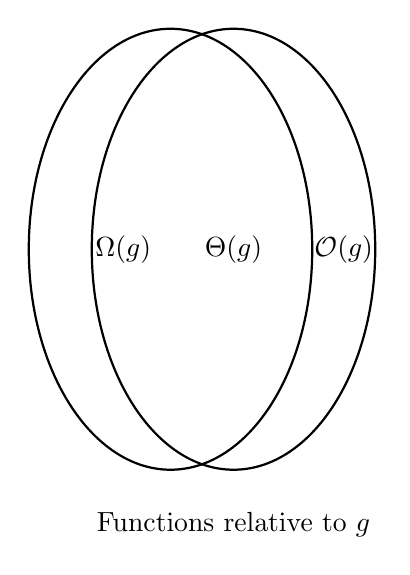
\begin{tikzpicture}
  \draw[thick] (0,0) ellipse (1.8cm and 2.8cm);
  \draw[thick] (0.8,0) ellipse (1.8cm and 2.8cm);
  \node at (-0.6, 0)  {$\Omega(g)$};
  \node at (0.8, 0)   {$\Theta(g)$};
  \node at (2.2, 0)   {$\mathcal{O}(g)$};
  \node at (0.8, -3.5) {Functions relative to $g$};
\end{tikzpicture}
\end{center}

% -----------------------------------------------------------------------------
\subsection{Big-Oh Notation (\texorpdfstring{$\mathcal{O}$}{O})}
\label{subsec:big-oh}
% -----------------------------------------------------------------------------

\begin{definition}[Big-Oh Notation]
\label{def:big-oh}
Let $f, g : \mathbb{N} \to \mathbb{R}^+$.  Then $f(n) \in \mathcal{O}(g(n))$
if $f(n)$ is \textbf{bounded above} by a constant multiple of $g(n)$ for all
sufficiently large $n$:
\[
  \mathcal{O}(g(n)) = \bigl\{f(n) : \exists\, c > 0,\; n_0 \text{ s.t.\ }
  0 \le f(n) \le c\,g(n)\; \forall\, n \ge n_0\bigr\}.
\]
Equivalently (limit definition):
\[
  f(n) \in \mathcal{O}(g(n)) \iff \lim_{n\to\infty}\frac{f(n)}{g(n)} < \infty.
\]
We say $g(n)$ is an \textbf{asymptotic upper bound} for $f(n)$.
\end{definition}

\begin{example}[Big-Oh examples]
\label{ex:big-oh-examples}
Let $f(n) = 4n + 3$.
\begin{itemize}
  \item $g(n) = n$: choose $c = 5$, $n_0 = 3$.  Then $4n+3 \le 5n$ for all $n \ge 3$.
        Hence $4n + 3 \in \mathcal{O}(n)$.  Verification via limit:
        $\lim_{n\to\infty}\frac{4n+3}{n} = 4 < \infty$. \checkmark
  \item $g(n) = n^3$: choose $c = 1$, $n_0 = 3$.  Then $4n+3 \le n^3$ for all $n \ge 3$.
        Hence $4n + 3 \in \mathcal{O}(n^3)$. \checkmark
  \item $g(n) = e^n$: applying L'H\^{o}pital's Rule,
        $\lim_{n\to\infty}\frac{4n+3}{e^n} = \lim_{n\to\infty}\frac{4}{e^n} = 0 < \infty$.
        Hence $4n + 3 \in \mathcal{O}(e^n)$. \checkmark
\end{itemize}
\end{example}

\begin{warning}[title={Warning: Big-Oh does not mean ``tight''}]
$f(n) \in \mathcal{O}(g(n))$ only guarantees an \emph{upper} bound.
$4n+3 \in \mathcal{O}(n^3)$ is true, but it is a loose bound.
For the tightest characterisation, use $\Theta$ notation.
\end{warning}

% -----------------------------------------------------------------------------
\subsection{Big-Omega Notation (\texorpdfstring{$\Omega$}{Omega})}
\label{subsec:big-omega}
% -----------------------------------------------------------------------------

\begin{definition}[Big-Omega Notation]
\label{def:big-omega}
Let $f, g : \mathbb{N} \to \mathbb{R}^+$.  Then $f(n) \in \Omega(g(n))$
if $f(n)$ is \textbf{bounded below} by a constant multiple of $g(n)$ for all
sufficiently large $n$:
\[
  \Omega(g(n)) = \bigl\{f(n) : \exists\, c > 0,\; n_0 \text{ s.t.\ }
  0 \le c\,g(n) \le f(n)\; \forall\, n \ge n_0\bigr\}.
\]
Equivalently (limit definition):
\[
  f(n) \in \Omega(g(n)) \iff \lim_{n\to\infty}\frac{f(n)}{g(n)} > 0
  \quad (\text{including } \infty).
\]
We say $g(n)$ is an \textbf{asymptotic lower bound} for $f(n)$.
\end{definition}

\begin{example}[Big-Omega example]
\label{ex:big-omega-example}
Let $f(n) = 4n + 3$ and $g(n) = n$.  Choose $c = 1$, $n_0 = 1$.
Then $4n + 3 \ge n$ for all $n \ge 1$, so $4n+3 \in \Omega(n)$.
Via limit: $\lim_{n\to\infty}\frac{4n+3}{n} = 4 > 0$. \checkmark
\end{example}

% -----------------------------------------------------------------------------
\subsection{Big-Theta Notation (\texorpdfstring{$\Theta$}{Theta})}
\label{subsec:big-theta}
% -----------------------------------------------------------------------------

\begin{definition}[Big-Theta Notation]
\label{def:big-theta}
Let $f, g : \mathbb{N} \to \mathbb{R}^+$.  Then $f(n) \in \Theta(g(n))$
if $f(n)$ is \textbf{bounded both above and below} by constant multiples
of $g(n)$ for all sufficiently large $n$:
\[
  \Theta(g(n)) = \bigl\{f(n) : \exists\, c_1, c_2 > 0,\; n_0 \text{ s.t.\ }
  c_1 g(n) \le f(n) \le c_2 g(n)\; \forall\, n \ge n_0\bigr\}.
\]
Equivalently (limit definition):
\[
  f(n) \in \Theta(g(n)) \iff \lim_{n\to\infty}\frac{f(n)}{g(n)} = c,
  \quad 0 < c < \infty.
\]
We say $g(n)$ is an \textbf{asymptotic tight bound} for $f(n)$.
\end{definition}

\begin{example}[Big-Theta example]
\label{ex:big-theta-example}
Let $f(n) = 4n + 3$ and $g(n) = n$.
$\lim_{n\to\infty}\frac{4n+3}{n} = 4$, and $0 < 4 < \infty$.
Hence $4n+3 \in \Theta(n)$.
\end{example}

% -----------------------------------------------------------------------------
\subsection{Summary: Limit-Based Classification}
\label{subsec:limit-summary}
% -----------------------------------------------------------------------------

\begin{keyresult}[title={Limit Rule for Asymptotic Classification}]
\[
  L = \lim_{n\to\infty}\frac{f(n)}{g(n)}
\]
\begin{center}
\begin{tabular}{@{}cccc@{}}
\toprule
$L$ & $f \in \mathcal{O}(g)$ & $f \in \Omega(g)$ & $f \in \Theta(g)$ \\
\midrule
$0$           & \checkmark & & \\
$0 < c < \infty$ & \checkmark & \checkmark & \checkmark \\
$\infty$      & & \checkmark & \\
\bottomrule
\end{tabular}
\end{center}
\end{keyresult}

% -----------------------------------------------------------------------------
\subsection{Simplification Rules}
\label{subsec:simplification-rules}
% -----------------------------------------------------------------------------

\begin{theorem}[Asymptotic Simplification Rules]
\label{thm:simplification}
\leavevmode
\begin{enumerate}
  \item \textbf{Constant scaling:} $f(n) = \mathcal{O}(c\,g(n)) \Rightarrow f(n) = \mathcal{O}(g(n))$
        for any constant $c > 0$.
  \item \textbf{Transitivity:} $f = \mathcal{O}(g)$ and $g = \mathcal{O}(h)$
        $\Rightarrow f = \mathcal{O}(h)$.
        \emph{e.g.}\ $2n = \mathcal{O}(n^2)$ and $n^2 = \mathcal{O}(n^3)$ implies
        $2n = \mathcal{O}(n^3)$.
  \item \textbf{Sum rule:} $f_1 = \mathcal{O}(g_1)$ and $f_2 = \mathcal{O}(g_2)$
        $\Rightarrow f_1 + f_2 = \mathcal{O}(\max(g_1, g_2))$.
        \emph{e.g.}\ $5n + 3\log_2 n = \mathcal{O}(n)$.
  \item \textbf{Product rule:} $f_1 = \mathcal{O}(g_1)$ and $f_2 = \mathcal{O}(g_2)$
        $\Rightarrow f_1 f_2 = \mathcal{O}(g_1 g_2)$.
        \emph{e.g.}\ $3n^2 \cdot \log_2 n = \mathcal{O}(n^2 \log_2 n)$.
\end{enumerate}
\end{theorem}

\begin{theorem}[Properties of Asymptotic Notation]
\label{thm:asym-properties}
\leavevmode
\begin{itemize}
  \item \textbf{Reflexivity} ($\mathcal{O}$, $\Omega$, $\Theta$):
        $f(n) = \mathcal{O}(f(n))$, etc.
  \item \textbf{Symmetry} ($\Theta$ only):
        $f = \Theta(g) \Leftrightarrow g = \Theta(f)$.
  \item \textbf{Transitivity} ($\mathcal{O}$, $\Omega$, $\Theta$):
        $f = \mathcal{O}(g)$ and $g = \mathcal{O}(h) \Rightarrow f = \mathcal{O}(h)$, etc.
\end{itemize}
\end{theorem}

% -----------------------------------------------------------------------------
\subsection{Asymptotic Notation in Equations}
\label{subsec:asym-in-eqns}
% -----------------------------------------------------------------------------

Asymptotic notation may appear inside equations as a shorthand for an
unspecified function of that complexity class.  For example:
\begin{itemize}
  \item $2n^2 + 3n + 1 = 2n^2 + \Theta(n)$: the $3n+1$ term is in $\Theta(n)$.
  \item $2n^2 + 3n + 1 = 2n^2 + \Theta(n) = \Theta(n^2)$: the dominant term is $n^2$.
  \item $T(n) = 2T\!\left(\tfrac{n}{2}\right) + \Theta(n)$: a recurrence for merge sort.
\end{itemize}

% -----------------------------------------------------------------------------
\section{Common Complexity Classes}
\label{sec:complexity-classes}
% -----------------------------------------------------------------------------

\begin{keyresult}[title={Standard Complexity Classes (slowest to fastest growth)}]
\begin{center}
\begin{tabularx}{\linewidth}{@{}l l X@{}}
\toprule
\textbf{Order} & \textbf{Class} & \textbf{Canonical Example} \\
\midrule
$\mathcal{O}(1)$           & Constant      & Finding midpoint of an array \\
$\mathcal{O}(\log n)$      & Logarithmic   & Binary search \\
$\mathcal{O}(n)$           & Linear        & Linear (sequential) search \\
$\mathcal{O}(n\log n)$     & Linearithmic  & Merge sort \\
$\mathcal{O}(n^2)$         & Quadratic     & Bubble sort, insertion sort \\
$\mathcal{O}(n^3)$         & Cubic         & Na\"{i}ve matrix inversion \\
$\mathcal{O}(2^n)$         & Exponential   & Recursive Fibonacci, Tower of Hanoi \\
$\mathcal{O}(n!)$          & Factorial     & Travelling Salesman (brute force) \\
\bottomrule
\end{tabularx}
\end{center}
\end{keyresult}

\begin{remark}
When the time complexity of algorithm $A$ grows faster than that of algorithm
$B$ for the same problem, we say $A$ is \textbf{inferior} to $B$.  In practice,
$\mathcal{O}$-notation is the most widely reported bound because it communicates
the worst-case guarantee.
\end{remark}

\paragraph{Worked derivation --- how to determine $\mathcal{O}$ from an algorithm:}
\begin{enumerate}
  \item Count primitive operations to obtain $f(n)$.
  \item Discard all constant terms and constant multipliers.
  \item Identify the \textbf{dominant term} (the fastest-growing term).
  \item The dominant term gives the $\mathcal{O}$-notation.
\end{enumerate}

% -----------------------------------------------------------------------------
\section{Space Complexity}
\label{sec:space-complexity}
% -----------------------------------------------------------------------------

Space complexity counts \textbf{basic storage units} (integers, floats,
characters) used by an algorithm.

\begin{example}[Array of $n$ integers]
\label{ex:space-array}
An array of $n$ integers requires $\Theta(n)$ space.
\end{example}

\begin{example}[Adjacency matrix for a graph]
\label{ex:space-matrix}
An $n \times n$ matrix used to store edge information for a graph with $n$
vertices (where $G[x][y] = 1$ iff there is an edge from $x$ to $y$) requires
$\Theta(n^2)$ space.
\end{example}

\begin{keyresult}[title={Space--Time Tradeoff Principle}]
There is typically an inverse relationship between time complexity and space
complexity.  Reducing time often requires storing pre-computed or intermediate
results (using more memory), and vice versa.  Algorithm designers frequently
exploit this tradeoff deliberately, e.g.\ memoisation (caches results for
constant-time lookup at the cost of $\Theta(n)$ extra space).
\end{keyresult}

% -----------------------------------------------------------------------------
\section{Summary}
\label{sec:aoa-summary}
% -----------------------------------------------------------------------------

\begin{keyresult}[title={Chapter Summary: Analysis of Algorithms}]
\begin{enumerate}
  \item \textbf{Time complexity} counts primitive operations as a function of
        input size $n$; \textbf{space complexity} counts storage units.
  \item For \emph{selection structures}, always state best-case, worst-case,
        and average-case separately.
  \item For \emph{recursive functions}, set up a recurrence relation and solve
        via backward substitution (unfold from $W_n$) or forward substitution
        (compute $W_1, W_2, \ldots$ and spot the pattern).
  \item \textbf{Order of growth} ignores constant factors; focus on the
        dominant term.
  \item $\mathcal{O}(g)$: upper bound ($f \le cg$).
        $\Omega(g)$: lower bound ($f \ge cg$).
        $\Theta(g)$: tight bound ($c_1 g \le f \le c_2 g$).
  \item Use the limit rule to classify:
        $L=0 \Rightarrow \mathcal{O}$;
        $0 < L < \infty \Rightarrow \Theta$ (and hence also $\mathcal{O}$ and $\Omega$);
        $L=\infty \Rightarrow \Omega$.
\end{enumerate}
\end{keyresult}

% =============================================================================
\chapter{Searching}
\label{ch:searching}
% =============================================================================

This chapter examines three fundamental searching algorithms, classified by their
design strategy: sequential search (a brute-force exhaustive approach), binary
search (a decrease-and-conquer strategy), and jump search (a compromise between
the two).  Each algorithm's time complexity is analysed under best-case,
average-case, and worst-case assumptions.

% -----------------------------------------------------------------------------
\section{Sequential Search}
\label{sec:sequential-search}
% -----------------------------------------------------------------------------

Sequential search (also called \emph{linear search}) is the simplest searching
strategy: traverse the data structure element by element, comparing each key
with the target until a match is found or the structure is exhausted.

\begin{lstlisting}[language=Python]
def search(head, a):
    pt = head
    while pt is not None and pt.key != a:
        pt = pt.next
    return pt
\end{lstlisting}

Because the data is stored \emph{unordered}, every element may need to be
inspected.  This makes sequential search a \textbf{brute-force} (na\"{\i}ve)
algorithm.

% -----------------------------------------------------------------------------
\subsection{Time Complexity of Sequential Search}
\label{subsec:seq-time}
% -----------------------------------------------------------------------------

Let $c_1$ denote the cost of the comparison and return when the target is found
immediately, and let $c_2$ denote the cost of one loop iteration (comparison
plus pointer advance).

\paragraph{Best case.}
The target is the first element.  Only the initial comparison executes, giving
a cost of $c_1$, hence $\Theta(1)$.

\paragraph{Worst case.}
The target is the last element (or absent).  The loop runs $n-1$ iterations
before the final comparison, costing $c_2(n-1) + c_1 = \Theta(n)$.

\paragraph{Average case (target present).}
Assume that every element is equally likely to be the target, so each
position~$i$ has probability $p_i = \tfrac{1}{n}$.  Finding the element at
position~$i$ costs $c_1 + (i-1)\,c_2$.  The expected cost is therefore:
\begin{align}
  A_s(n) &= \sum_{i=1}^{n} \frac{1}{n}\bigl[c_1 + (i-1)\,c_2\bigr]
          = \frac{1}{n}\left[n\,c_1 + c_2\sum_{i=1}^{n}(i-1)\right] \notag \\
         &= \frac{1}{n}\left[n\,c_1 + c_2 \cdot \frac{n(n-1)}{2}\right]
          = c_1 + \frac{c_2(n-1)}{2} = \Theta(n). \label{eq:seq-avg}
\end{align}

\paragraph{Average case (target may be absent).}
If the target is absent, the full list is scanned at cost $c_1 + n\,c_2 = \Theta(n)$.
Letting $q = P(\text{target in list})$, the overall average is:
\[
  A(n) = q\left(c_1 + \frac{c_2(n-1)}{2}\right) + (1-q)(c_1 + n\,c_2),
\]
which remains a linear function of~$n$, so the average-case complexity is
$\Theta(n)$ regardless of~$q$.

\begin{keyresult}[title={Sequential Search Complexity}]
Sequential search runs in $\mathcal{O}(n)$ time.  Best case is $\Theta(1)$;
worst and average cases are both $\Theta(n)$.  The data need not be sorted.
\end{keyresult}

% -----------------------------------------------------------------------------
\section{Binary Search}
\label{sec:binary-search}
% -----------------------------------------------------------------------------

Binary search exploits a \textbf{sorted} list by repeatedly halving the search
interval --- a classic \emph{decrease-and-conquer} strategy.

\subsection{Recursive Implementation}
\label{subsec:binsearch-recursive}

\begin{lstlisting}[language=Python]
def binary_search_recursive(arr, left, right, target):
    if left > right:
        return -1
    mid = left + (right - left) // 2
    if arr[mid] == target:
        return mid
    elif arr[mid] < target:
        return binary_search_recursive(
            arr, mid + 1, right, target)
    else:
        return binary_search_recursive(
            arr, left, mid - 1, target)
\end{lstlisting}

\subsection{Iterative Implementation}
\label{subsec:binsearch-iterative}

\begin{lstlisting}[language=Python]
def binary_search(arr, target):
    low = 0
    high = len(arr) - 1
    while low <= high:
        mid = (low + high) // 2
        if arr[mid] == target:
            return mid
        elif arr[mid] < target:
            low = mid + 1
        else:
            high = mid - 1
    return -1
\end{lstlisting}

% -----------------------------------------------------------------------------
\subsection{Connection to Binary Search Trees}
\label{subsec:binsearch-bst}
% -----------------------------------------------------------------------------

A sorted list can be viewed as the in-order traversal of a \textbf{binary
search tree} (BST).  For example, the sorted list $[14, 23, 31, 56, 73, 93, 94]$
corresponds to the following BST with root~56:

% [Figure, Slide 9: BST built from sorted list 14,23,31,56,73,93,94]
\begin{figure}[h]
\centering
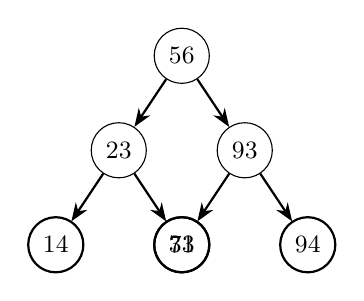
\begin{tikzpicture}[
    every node/.style={draw, circle, minimum size=7mm, inner sep=1pt,
                       font=\small},
    level distance=12mm, sibling distance=16mm,
    edge from parent/.style={draw, -{Stealth}, thick}
  ]
  \node {56}
    child { node {23}
      child { node {14} }
      child { node {31} }
    }
    child { node {93}
      child { node {73} }
      child { node {94} }
    };
\end{tikzpicture}
\caption{BST corresponding to the sorted list $[14,23,31,56,73,93,94]$.}
\label{fig:bst-sorted}
\end{figure}

Binary search on the array is equivalent to traversing from the root towards a
leaf in the BST, making one comparison per level.  An alternative recursive
formulation using BST node traversal is:

\begin{lstlisting}[language=Python]
def binary_search(self, target, current_node):
    if current_node is None:
        return False
    elif target == current_node.data:
        return True
    elif target < current_node.data:
        return self.binary_search(
            target, current_node.left)
    else:
        return self.binary_search(
            target, current_node.right)
\end{lstlisting}

% -----------------------------------------------------------------------------
\subsection{Tree Height and Node Count}
\label{subsec:tree-height}
% -----------------------------------------------------------------------------

\begin{definition}[Height and Depth]
\label{def:height-depth}
The \textbf{height} of a tree is the number of edges on the longest path from
the root to a leaf.  The \textbf{depth} of a node is the number of edges from
that node to the root.
\end{definition}

For a \emph{complete} binary tree of height $H$, the number of nodes $n$
satisfies:
\[
  2^{H} \le n < 2^{H+1}.
\]
Taking logarithms gives $H \le \log_2 n < H+1$, and since $H$ is an integer we
obtain:
\[
  H = \lfloor \log_2 n \rfloor.
\]

% -----------------------------------------------------------------------------
\subsection{Worst-Case Time Complexity}
\label{subsec:binsearch-worst}
% -----------------------------------------------------------------------------

Assume a complete binary tree with $n$ nodes.  Let $f(n)$ denote the worst-case
number of operations.  At each step, a constant amount of work~$c$ is done,
then the problem is reduced to a subtree of size $\tfrac{n-1}{2}$.  This gives
the recurrence:
\[
  f(n) = f\!\left(\frac{n-1}{2}\right) + c.
\]
Unfolding $k$ times:
\begin{align}
  f(n) &= f\!\left(\frac{n - (2^k - 1)}{2^k}\right) + kc. \label{eq:binsearch-unfold}
\end{align}
The recursion bottoms out when the argument equals~1, i.e.\ when
$\frac{n - (2^k - 1)}{2^k} = 1$, which gives $2^k = \frac{n+1}{2}$, so
$k = \log_2(n+1) - 1 = \lfloor \log_2 n \rfloor$.  Substituting back:
\[
  f(n) = f(1) + kc = c + \lfloor \log_2 n \rfloor \cdot c
       = (\lfloor \log_2 n \rfloor + 1)\,c = \Theta(\log_2 n).
\]

\begin{examtip}[title={Deriving Binary Search Complexity}]
Set up the recurrence $f(n) = f\!\bigl(\frac{n-1}{2}\bigr) + c$, unfold $k$ times
to get $f(n) = f\!\bigl(\frac{n-(2^k-1)}{2^k}\bigr) + kc$, then solve for $k$
by setting the argument to~1.  The result is $k = \lfloor\log_2 n\rfloor$ and
$f(n) = \Theta(\log_2 n)$.
\end{examtip}

% -----------------------------------------------------------------------------
\subsection{Average-Case Time Complexity}
\label{subsec:binsearch-avg}
% -----------------------------------------------------------------------------

Let $A_s(n)$ and $A_f(n)$ denote the average number of comparisons for a
successful and unsuccessful search respectively.  The overall average is
$A(n) = q\,A_s(n) + (1-q)\,A_f(n)$, where $q$ is the probability the target
is present.

\paragraph{Unsuccessful search.}
An unsuccessful search always reaches a leaf, traversing the full height of the
tree, so $A_f(n) = \Theta(\log_2 n)$.

\paragraph{Successful search.}
Assume $n = 2^k - 1$ (a complete binary tree).  At level~$t$ of the tree there
are $2^{t-1}$ nodes, each requiring exactly $t$~comparisons.  Under the uniform
distribution ($p_i = \tfrac{1}{n}$):
\[
  A_s(n) = \frac{1}{n}\sum_{t=1}^{k} t \cdot 2^{t-1}.
\]

To evaluate $\sum_{t=1}^{k} t\cdot 2^{t-1}$, we use the perturbation method.
Let $S = \sum_{t=1}^{k} t\cdot 2^{t-1}$.  Multiplying by~2 and subtracting:
\begin{align*}
  S &= 1\cdot 1 + 2\cdot 2 + 3\cdot 4 + \cdots + k\cdot 2^{k-1}, \\
  2S &= \phantom{1\cdot 1 + {}} 1\cdot 2 + 2\cdot 4 + \cdots + (k-1)\cdot 2^{k-1} + k\cdot 2^k.
\end{align*}
Subtracting gives $(2-1)S = k\cdot 2^k - (1 + 2 + 4 + \cdots + 2^{k-1})
= k\cdot 2^k - (2^k - 1)$, so:
\[
  S = (k-1)\,2^k + 1.
\]
Therefore:
\[
  A_s(n) = \frac{(k-1)\,2^k + 1}{n}
         = \frac{[\log_2(n+1) - 1](n+1) + 1}{n}
         = \log_2(n+1) - 1 + \frac{\log_2(n+1)}{n}.
\]

\paragraph{Overall average.}
Since $q \le 1$ and $\frac{\log_2(n+1)}{n}$ is negligible for large~$n$:
\[
  A(n) = q\,A_s(n) + (1-q)\,A_f(n) = \Theta(\log_2 n).
\]

\begin{keyresult}[title={Binary Search Complexity}]
Binary search runs in $\mathcal{O}(\log_2 n)$ time.  Best case is $\Theta(1)$
(target at the midpoint); worst and average cases are both $\Theta(\log_2 n)$.
\textbf{Prerequisite:} the input must be sorted.
\end{keyresult}

\begin{warning}[title={Binary Search Requires Sorted Input}]
Binary search only produces correct results on a sorted array (or equivalently,
a valid BST).  Applying it to unsorted data silently yields incorrect answers
--- the algorithm does not detect unsorted input.
\end{warning}

\begin{examtip}[title={Complete/Balanced BST Required for $O(\log n)$}]
The $O(\log_2 n)$ complexity of binary search on a BST assumes the tree is
\emph{complete} or \emph{balanced}.  A degenerate BST---where each node has
only one child---reduces to a linked list, and binary search degrades to
$O(n)$.  To guarantee logarithmic search time, use a balanced BST such as an
AVL tree (Chapter~\ref{ch:avl-trees}).
\end{examtip}

% -----------------------------------------------------------------------------
\section{Jump Search}
\label{sec:jump-search}
% -----------------------------------------------------------------------------

Jump search is a searching algorithm for sorted arrays that reduces the number
of comparisons relative to sequential search by ``jumping'' ahead in fixed-size
blocks of $\lfloor\sqrt{n}\rfloor$ elements, then performing a linear scan
within the identified block.  It is particularly useful when binary search is
costly --- for example, when searching a very large sorted dataset stored on a
slow storage medium such as a disk-based database.

\begin{lstlisting}[language=Python]
import math

def jump_search(arr, target):
    n = len(arr)
    step = int(math.sqrt(n))
    prev = 0
    while prev < n and arr[min(step, n) - 1] < target:
        prev = step
        step += int(math.sqrt(n))
        if prev >= n:
            return -1
    for i in range(prev, min(step, n)):
        if arr[i] == target:
            return i
    return -1
\end{lstlisting}

% -----------------------------------------------------------------------------
\subsection{Time Complexity of Jump Search}
\label{subsec:jump-time}
% -----------------------------------------------------------------------------

The algorithm operates in two phases: a \emph{jump phase} that skips through at
most $\frac{n}{\sqrt{n}} = \sqrt{n}$ blocks, and a \emph{linear scan phase}
within a single block of size at most $\sqrt{n}$.

\paragraph{Best case.}
The target is at the start of the array: $\Theta(1)$.

\paragraph{Worst case.}
The jump phase inspects up to $\sqrt{n}$ block boundaries, and the linear scan
checks up to $\sqrt{n}$ elements within the final block, giving
$\Theta(\sqrt{n}) + \Theta(\sqrt{n}) = \Theta(\sqrt{n})$.

\paragraph{Average case.}
Under the uniform distribution, each element is equally likely, and the expected
number of comparisons is:
\[
  \sum_{i=1}^{n} \frac{1}{n}\,\Theta\!\left(\sqrt{n}\right) = \Theta\!\left(\sqrt{n}\right).
\]

\begin{keyresult}[title={Jump Search Complexity}]
Jump search runs in $\mathcal{O}(\sqrt{n})$ time.  It sits between sequential
search ($\mathcal{O}(n)$) and binary search ($\mathcal{O}(\log n)$) in
efficiency.  Like binary search, it requires sorted input.
\end{keyresult}

% -----------------------------------------------------------------------------
\section{Summary}
\label{sec:searching-summary}
% -----------------------------------------------------------------------------

The following table compares the three searching algorithms discussed in this
chapter.

\begin{center}
\begin{tabularx}{\linewidth}{@{}l *{3}{>{\centering\arraybackslash}X} c@{}}
\toprule
\textbf{Algorithm} & \textbf{Best} & \textbf{Average} & \textbf{Worst} & \textbf{Overall} \\
\midrule
Sequential & $\Theta(1)$          & $\Theta(n)$          & $\Theta(n)$          & $\mathcal{O}(n)$          \\
Binary     & $\Theta(1)$          & $\Theta(\log_2 n)$   & $\Theta(\log_2 n)$   & $\mathcal{O}(\log_2 n)$   \\
Jump       & $\Theta(1)$          & $\Theta(\sqrt{n})$   & $\Theta(\sqrt{n})$   & $\mathcal{O}(\sqrt{n})$   \\
\bottomrule
\end{tabularx}
\end{center}

Sequential search is a brute-force exhaustive algorithm that requires no
assumptions about the data ordering.  Binary search and jump search are both
decrease-and-conquer algorithms that require the input to be sorted.  Binary
search achieves the best asymptotic complexity of the three at
$\mathcal{O}(\log_2 n)$, but jump search can be preferable in practice when
random access is expensive (e.g.\ data on disk), since it performs fewer
large jumps followed by a short sequential scan.

\chapter{Hash Tables}
\label{ch:hash-tables}

The search algorithms discussed in Chapter~\ref{ch:searching} achieve at best
$O(\log n)$ time (binary search) for sorted data.  \emph{Hash tables} take a
fundamentally different approach: they trade space for time, using a
\textbf{hash function} to map keys directly to array indices, achieving
$O(1)$ average-case lookup, insertion, and deletion.

\section{Direct-Address Tables}
\label{sec:direct-address}

\begin{definition}[Direct-Address Table]
\label{def:direct-address}
Suppose the set of actual keys $K$ is drawn from a universe
$U = \{0, 1, 2, \ldots, m-1\}$ and all keys are distinct.  A
\emph{direct-address table} is an array $T[0 \ldots m-1]$ where
\[
  T[k] =
  \begin{cases}
    x & \text{if } k \in K \text{ and } x.\mathit{key} = k, \\
    \texttt{NIL} & \text{otherwise.}
  \end{cases}
\]
\end{definition}

All operations---search, insert, delete---run in $O(1)$ time because the key
itself is the index.  However, direct-address tables are impractical when the
universe $U$ is much larger than the set of actual keys ($|U| \gg |K|$).  For
example, if keys are 64-bit integers, the table would need $\approx 1.8 \times
10^{19}$ entries regardless of how few keys are actually stored.

% [Figure, Slide: Direct-address table mapping actual keys K (subset of
% universe U) to array slots, with unoccupied slots set to NIL.]

\begin{figure}[h]
\centering
\resizebox{0.85\linewidth}{!}{%
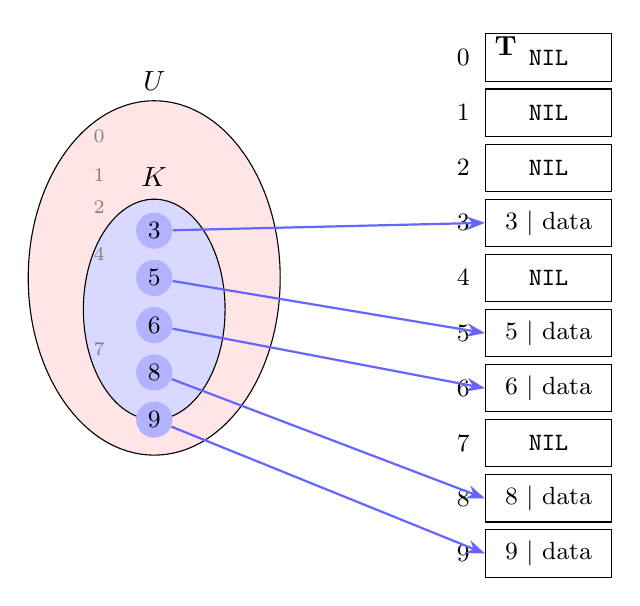
\begin{tikzpicture}[
    slot/.style={draw, rectangle, minimum width=1.6cm, minimum height=0.6cm,
                 anchor=west},
    arr/.style={-{Stealth}, thick}
  ]
  % Hash table
  \foreach \i/\content in {0/\texttt{NIL},1/\texttt{NIL},2/\texttt{NIL},
                           3/{3 $|$ data},4/\texttt{NIL},5/{5 $|$ data},
                           6/{6 $|$ data},7/\texttt{NIL},8/{8 $|$ data},
                           9/{9 $|$ data}} {
    \node[slot] (s\i) at (5, -0.7*\i) {\small \content};
    \node[left=2pt of s\i, anchor=east] {\small \i};
  }
  \node[above=4pt of s0.west, anchor=west] {\textbf{T}};
  % Universe ellipse
  \node[draw, ellipse, minimum width=3.2cm, minimum height=4.5cm,
        fill=red!10] (U) at (0.8, -2.8) {};
  \node[above] at (U.north) {$U$};
  % Actual keys ellipse
  \node[draw, ellipse, minimum width=1.8cm, minimum height=2.8cm,
        fill=blue!15] (K) at (0.8, -3.2) {};
  \node[above=1pt] at (K.north) {$K$};
  % Keys
  \foreach \k/\y in {3/-2.2, 5/-2.8, 6/-3.4, 8/-4.0, 9/-4.6} {
    \node[fill=blue!30, circle, inner sep=2pt, font=\small] (k\k) at (0.8, \y) {\k};
    \draw[arr, blue!60] (k\k) -- (s\k.west);
  }
  % Non-keys
  \foreach \k/\y in {0/-1.0, 1/-1.5, 2/-1.9, 4/-2.5, 7/-3.7} {
    \node[font=\scriptsize, gray] at (0.1, \y) {\k};
  }
\end{tikzpicture}%
}
\caption{Direct-address table: each key maps directly to its index.}
\label{fig:direct-address}
\end{figure}

% -----------------------------------------------------------------------
\section{Hashing}
\label{sec:hashing}

To overcome the space problem of direct addressing, we use a \emph{hash
function} $h$ that maps the universe $U$ of all possible keys into a
smaller range of hash table slots:
\[
  h\colon U \to \{0, 1, 2, \ldots, m-1\}.
\]

\begin{definition}[Hash Table and Load Factor]
\label{def:hash-table}
A \emph{hash table} is an array of $m$ slots indexed $0, 1, \ldots, m-1$.
A key $k$ is stored at index $h(k)$.  If $n$ keys are stored in a table of
size $m$, the \emph{load factor} is $\alpha = n/m$.
\end{definition}

Because the domain of $h$ is typically much larger than its range, multiple
keys may map to the same slot.  This event is called a \emph{collision}.

% -----------------------------------------------------------------------
\section{Hash Functions}
\label{sec:hash-functions}

A good hash function should satisfy three properties: it must map every
possible key to a valid table index; it should distribute keys as evenly as
possible across slots; and it should be fast to compute.

\subsection{Division Method (Modulo Arithmetic)}
\label{subsec:hash-division}

The simplest hash function divides the key by the table size and takes the
remainder:
\[
  h(k) = k \bmod m.
\]

\begin{example}[Division Method]
\label{ex:hash-division}
With $m = 13$ and $k = 37699$: $h(37699) = 37699 \bmod 13 = 12$.
\end{example}

\begin{examtip}[title={Choosing $m$ for the Division Method}]
Avoid powers of 10 (for decimal keys) and powers of 2 (when lower bit
patterns are non-uniform).  The best choice of $m$ is a \textbf{prime number}
not too close to any power of~2, as this distributes keys most evenly.
\end{examtip}

\subsection{Folding Method}
\label{subsec:hash-folding}

The key is partitioned into several parts, which are then combined
(typically by addition) and taken modulo~$m$:
\[
  h(k) = (k_1 + k_2 + \cdots + k_p) \bmod m,
\]
where $k_1, k_2, \ldots, k_p$ are fixed-width segments of~$k$.

\begin{example}[Shift Folding]
\label{ex:hash-folding}
With $m = 13$ and $k = 123456789$, partition into 3-digit groups:
$h(123456789) = (123 + 456 + 789) \bmod 13 = 1368 \bmod 13 = 3$.
This method is especially useful for very long keys (e.g.\ 20-digit numbers).
\end{example}

\begin{lstlisting}[language=C]
// Folding hash for a 10-character key
int h(char x[10]) {
    int i, sum;
    for (sum = 0, i = 0; i < 10; i++)
        sum += (int) x[i];
    return (sum % M);
}
\end{lstlisting}

\subsection{Mid-Square Method}
\label{subsec:hash-midsquare}

The key is squared, and the middle $r$ bits (or digits) of the result are
extracted as the hash value for a table of $2^r$ slots.

\begin{example}[Mid-Square]
\label{ex:hash-midsquare}
With $k = 3121$: $k^2 = 9{,}740{,}641$.  Extracting the middle three digits
gives $h(k) = 406$.
\end{example}

\subsection{Multiplicative Congruential Method}
\label{subsec:hash-mcm}

A pseudo-random multiplier $a$ is used:
\[
  h(k) = (a \times k) \bmod m.
\]

\begin{example}[Multiplicative Congruential]
\label{ex:hash-mcm}
With $m = 31$ and $a = 8\lfloor m/23 \rfloor + 5 = 8(1) + 5 = 13$,
the keys $k = 1, 2, \ldots, 15$ map to
$13, 26, 8, 21, 3, 16, 29, 11, 24, 6, 19, 1, 14, 27, 9$ respectively---a
well-spread distribution.
\end{example}

% -----------------------------------------------------------------------
\section{Collision Resolution}
\label{sec:collision-resolution}

When two keys $k_1 \neq k_2$ satisfy $h(k_1) = h(k_2)$, a \emph{collision}
occurs.  Two families of strategies handle collisions: \emph{closed
addressing} (the key stays at its hashed slot, with overflow stored in a
linked list) and \emph{open addressing} (the key probes for an alternative
slot within the table).

% -----------------------------------------------------------------------
\subsection{Closed Addressing: Separate Chaining}
\label{subsec:closed-addressing}

Each slot in the hash table points to a linked list (a \emph{chain}).  All
keys that hash to the same index are appended to that slot's list.

\begin{figure}[h]
\centering
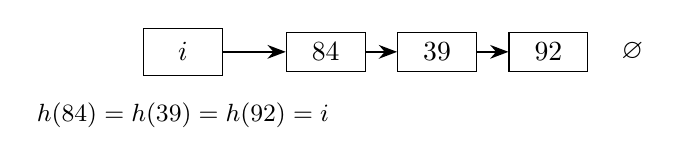
\begin{tikzpicture}[
    slot/.style={draw, rectangle, minimum width=1cm, minimum height=0.6cm},
    node/.style={draw, rectangle, minimum width=1cm, minimum height=0.5cm},
    arr/.style={-{Stealth}, thick}
  ]
  % Table slots (showing only slot i)
  \node[slot] (si) at (0,0) {$i$};
  % Chain
  \node[node, right=0.8cm of si] (n1) {84};
  \node[node, right=0.4cm of n1] (n2) {39};
  \node[node, right=0.4cm of n2] (n3) {92};
  \draw[arr] (si.east) -- (n1.west);
  \draw[arr] (n1.east) -- (n2.west);
  \draw[arr] (n2.east) -- (n3.west);
  \node[right=0.3cm of n3] {$\varnothing$};
  \node[below=6pt of si, font=\small] {$h(84) = h(39) = h(92) = i$};
\end{tikzpicture}
\caption{Separate chaining: keys 84, 39, 92 all hash to slot~$i$.}
\label{fig:chaining}
\end{figure}

\subsubsection{Python Implementation}
\label{subsubsec:chaining-impl}

The following implementation uses a linked list at each slot, with insert,
search, and delete operations:

\begin{lstlisting}[language=Python]
class HashTableNode:
    def __init__(self, key):
        self.key = key
        self.next = None

class HashTable:
    def __init__(self, num_data):
        self.load_factor = 3
        self.size = max(1, num_data // self.load_factor)
        self.table = [None] * self.size

    def _hash(self, key):
        return hash(key) % self.size

    def hash_insert(self, key):
        index = self._hash(key)
        head = self.table[index]
        if head is None:
            self.table[index] = HashTableNode(key)
            return True
        current = head
        while True:
            if current.key == key:
                return False  # duplicate
            if current.next is None:
                break
            current = current.next
        current.next = HashTableNode(key)
        return True

    def hash_search(self, key):
        index = self._hash(key)
        current = self.table[index]
        while current:
            if current.key == key:
                return True
            current = current.next
        return False

    def hash_delete(self, key):
        index = self._hash(key)
        current = self.table[index]
        prev = None
        while current:
            if current.key == key:
                if prev is None:
                    self.table[index] = current.next
                else:
                    prev.next = current.next
                return True
            prev = current
            current = current.next
        return False
\end{lstlisting}

\subsubsection{Worst-Case Analysis}
\label{subsubsec:chaining-worst}

The worst case occurs when \emph{all} $n$ keys hash to the same slot, producing
a single chain of length~$n$.  Searching then degenerates to sequential search
(cf.\ Section~\ref{sec:sequential-search}):

\begin{itemize}
  \item \textbf{Unsuccessful search}: $n$ key comparisons, $\Theta(n)$.
  \item \textbf{Successful search}: assuming equal probability $1/n$ for each
        key, the expected number of comparisons is
        $\frac{1}{n}\sum_{i=1}^{n} i = \frac{n+1}{2} = \Theta(n)$.
\end{itemize}

\subsubsection{Average-Case Analysis}
\label{subsubsec:chaining-avg}

\begin{theorem}[Average-Case Complexity of Chained Hashing]
\label{thm:chaining-avg}
Under the assumption that each key is equally likely to hash into any of the
$m$ slots (simple uniform hashing):
\begin{enumerate}
  \item An \textbf{unsuccessful search} examines $\alpha = n/m$ keys on
        average, since it must traverse an entire chain whose expected length
        is~$\alpha$.
  \item A \textbf{successful search} examines $\Theta(1 + \alpha)$ keys on
        average.
\end{enumerate}
\end{theorem}

\begin{proof}
For a successful search, when the $i$-th key is inserted, the average chain
length is $(i-1)/m$.  Therefore the expected number of comparisons to find the
$i$-th key later is $1 + (i-1)/m$.  Averaging over all $n$ keys:
\[
  A_s(n) = \frac{1}{n}\sum_{i=1}^{n}\left(1 + \frac{i-1}{m}\right)
         = 1 + \frac{1}{nm}\sum_{i=0}^{n-1} i
         = 1 + \frac{n-1}{2m}.
\]
Since $\alpha = n/m$, this is $1 + \frac{\alpha}{2} - \frac{1}{2m}
= \Theta(1 + \alpha)$.
\end{proof}

\begin{keyresult}[title={Key Result: Chained Hashing Performance}]
If $n$ is proportional to $m$ (i.e.\ $n = O(m)$), then $\alpha = O(1)$ and
both successful and unsuccessful searches take $\Theta(1)$ expected time.
This is the power of hashing: \textbf{constant-time search on average}.
\end{keyresult}

% -----------------------------------------------------------------------
\subsection{Open Addressing}
\label{subsec:open-addressing}

In open addressing, all keys are stored directly in the hash table (no
linked lists).  Consequently, the load factor satisfies $\alpha \le 1$.  When
a collision occurs at slot $h(k)$, a \emph{probe sequence} is followed to
find an empty slot.

\subsubsection{Linear Probing}
\label{subsubsec:linear-probing}

The probe function is:
\[
  H(k, i) = \bigl(H'(k) + i\bigr) \bmod m, \quad i = 0, 1, 2, \ldots, m-1,
\]
where $H'(k)$ is the auxiliary hash function (e.g.\ $H'(k) = k \bmod m$).

\begin{example}[Linear Probing]
\label{ex:linear-probing}
With $H(k,i) = (k + i) \bmod 7$, $H'(k) = k \bmod 7$, and
keys $\{4, 13, 19, 11\}$:

$H(4,0) = 4$; slot~4 is empty $\to$ insert 4 at slot~4.

$H(13,0) = 6$; slot~6 is empty $\to$ insert 13 at slot~6.

$H(19,0) = 5$; slot~5 is empty $\to$ insert 19 at slot~5.

$H(11,0) = 4$; slot~4 is occupied (by~4).
$H(11,1) = 5$; slot~5 is occupied (by~19).
$H(11,2) = 6$; slot~6 is occupied (by~13).
$H(11,3) = 0$; slot~0 is empty $\to$ insert 11 at slot~0.
\end{example}

\begin{warning}[title={Primary Clustering}]
Linear probing suffers from \emph{primary clustering}: long runs of occupied
slots build up, increasing both search and insertion time.  Keys that hash
to any slot in a cluster must probe to the end of the cluster, and the
cluster grows with each insertion.
\end{warning}

\subsubsection{Quadratic Probing}
\label{subsubsec:quadratic-probing}

The probe function introduces a quadratic term:
\[
  H(k, i) = \bigl(H'(k) + c_1 i + c_2 i^2\bigr) \bmod m,
  \quad c_2 \neq 0, \quad i = 0, 1, \ldots, m-1.
\]
The constants $c_1$, $c_2$, and $m$ must be chosen carefully so that all
slots are visited.  For $m = 2^p$, a good choice is $c_1 = c_2 = \tfrac{1}{2}$.

\begin{example}[Quadratic Probing]
\label{ex:quadratic-probing}
With $H(k,i) = \bigl(H'(k) + \tfrac{1}{2}i + \tfrac{1}{2}i^2\bigr) \bmod 8$
and $H'(k) = k \bmod 8$, the probe offsets for $i = 1, 2, \ldots, 7$ are
$1, 3, 6, 2, 7, 5, 4$---covering all slots.
\end{example}

Quadratic probing avoids primary clustering but introduces \emph{secondary
clustering}: if two keys have the same initial hash value $H'(k)$, their
probe sequences are identical.

\subsubsection{Double Hashing}
\label{subsubsec:double-hashing}

A second hash function determines the probe step size, producing a more
randomised probe sequence:
\[
  H(k, i) = \bigl(H_1(k) + i \cdot H_2(k)\bigr) \bmod m,
  \quad i = 0, 1, \ldots, m-1.
\]
Here $H_1$ and $H_2$ are both auxiliary hash functions, and $m$ should be
prime to ensure full table coverage.

\begin{example}[Double Hashing]
\label{ex:double-hashing}
With $m = 7$, $H_1(k) = k \bmod 7$, $H_2(k) = (k \bmod 3) + 1$, and
keys $\{0, 4, 13, 19, 11\}$:

$H(0,0) = 0$ $\to$ slot~0.

$H(4,0) = 4$ $\to$ slot~4.

$H(13,0) = 6$ $\to$ slot~6.

$H(19,0) = 5$ $\to$ slot~5.

$H(11,0) = 4$ (collision with~4); $H_2(11) = (11 \bmod 3)+1 = 3$,
so $H(11,1) = (4 + 3) \bmod 7 = 0$ (collision with~0);
$H(11,2) = (4 + 6) \bmod 7 = 3$ $\to$ slot~3.
\end{example}

% -----------------------------------------------------------------------
\subsubsection{Searching Under Open Addressing}
\label{subsubsec:open-search}

The search algorithm probes slots until the key is found, an empty slot is
reached (key absent), or all slots have been checked:

\begin{lstlisting}[language=Python]
def hash_search(table, k, hash_fn, probe_fn, m):
    code = hash_fn(k)
    loc = code
    while table[loc] is not None:
        if table[loc].key == k:
            return loc       # found
        loc = probe_fn(loc)
        if loc == code:
            break            # full cycle
    return None              # not found
\end{lstlisting}

Three outcomes are possible: the key is found (success), an empty slot is
reached (failure), or every slot has been probed without a match (failure).

% -----------------------------------------------------------------------
\subsection{Time Complexity of Open Addressing}
\label{subsec:open-addressing-tc}

The expected number of probes depends on the probing strategy and the load
factor~$\alpha$.

\begin{center}
\begin{tabularx}{\linewidth}{@{}l >{$}X<{$} >{$}X<{$}@{}}
\toprule
\textbf{Method} & \textbf{Successful Search}
                & \textbf{Unsuccessful Search} \\
\midrule
Linear Probing
  & \dfrac{1}{2}\!\left(1 + \dfrac{1}{1-\alpha}\right)
  & \dfrac{1}{2}\!\left(1 + \left(\dfrac{1}{1-\alpha}\right)^{\!2}\right) \\[12pt]
Double Hashing
  & \dfrac{1}{\alpha}\ln\!\dfrac{1}{1-\alpha}
  & \dfrac{1}{1-\alpha} \\
\bottomrule
\end{tabularx}
\end{center}

All expressions are functions of $\frac{1}{1-\alpha}$, which grows rapidly as
$\alpha \to 1$.  This means that performance degrades sharply when the table is
nearly full.

\begin{examtip}[title={Why Performance Degrades as $\alpha \to 1$}]
As the load factor approaches~1, nearly every slot is occupied and each
probe is likely to hit another key, causing long chains of probes.  The
expressions $\frac{1}{1-\alpha}$ and $\left(\frac{1}{1-\alpha}\right)^2$
diverge as $\alpha \to 1$, explaining why open-address hash tables must be
kept well below full capacity.
\end{examtip}

% -----------------------------------------------------------------------
\section{Deletion Under Open Addressing}
\label{sec:hash-deletion}

Deleting a key from an open-addressing hash table is more involved than in
chaining.  Simply emptying a slot would break the probe chain for any key
that was inserted after the deleted one and probed through that slot.

The standard solution is \textbf{lazy deletion}: mark the slot as
\emph{deleted} (often called a ``tombstone'') rather than emptying it.
Tombstoned slots are treated as occupied during search (so the probe chain
is not broken) but as empty during insertion (so new keys can reuse them).

After a large number of deletions, the table may accumulate many tombstones,
degrading search performance.  A periodic \emph{garbage collection} pass---
re-inserting all live keys into a clean table---restores efficiency.

% -----------------------------------------------------------------------
\section{Rehashing}
\label{sec:rehashing}

As $\alpha$ increases, search and insertion become slower regardless of the
probing strategy.  \emph{Rehashing} addresses this by allocating a larger
table (typically doubling the size to the next prime) and re-inserting every
existing key using the new hash function.  This resets the load factor to
approximately $\alpha/2$ and eliminates any tombstones.

% -----------------------------------------------------------------------
\section{Summary}
\label{sec:hash-summary}

\begin{keyresult}[title={Key Result: Hash Table Performance}]
\begin{enumerate}
  \item A \textbf{direct-address table} provides $O(1)$ operations but
        requires $|U|$ space, which is impractical for large key universes.
  \item \textbf{Hashing} compresses the key space via a hash function,
        achieving $O(1)$ average-case performance with $O(m)$ space.
  \item \textbf{Separate chaining} (closed addressing) handles collisions with
        linked lists; average search is $\Theta(1 + \alpha)$.
  \item \textbf{Open addressing} stores all keys in the table itself
        ($\alpha \le 1$); performance depends on the probing strategy and
        degrades as $\alpha \to 1$.
  \item Good hash function design (prime table sizes, avoiding powers of~2)
        and keeping $\alpha$ low via rehashing are essential for maintaining
        constant-time operations.
\end{enumerate}
\end{keyresult}

% =======================================================================
\chapter{Tries}
\label{ch:tries}

A \emph{trie} (also called a \textbf{prefix tree} or \textbf{digital tree})
is a tree-based data structure designed for efficient string operations.
Unlike the hash tables of Chapter~\ref{ch:hash-tables}, which map individual
keys to slots, a trie exploits the \emph{shared prefix structure} of a
collection of strings: characters common to multiple keys are stored only
once along shared edges from the root.

\begin{definition}[Trie]
\label{def:trie}
A \emph{trie} over an alphabet~$\Sigma$ is a rooted tree in which
\begin{enumerate}
  \item every edge is labelled with exactly one character from~$\Sigma$,
  \item no node has two outgoing edges with the same label, and
  \item a boolean flag \texttt{is\_end\_of\_word} marks which nodes correspond
        to the final character of a stored string.
\end{enumerate}
Searching or inserting a string of length~$L$ takes $O(L)$ time,
independent of the total number of strings stored.
\end{definition}

For example, the strings \texttt{bear}, \texttt{bell}, \texttt{bid},
\texttt{buy}, \texttt{car}, \texttt{care}, and \texttt{camp} produce the
trie shown in Figure~\ref{fig:trie-example}.

\begin{figure}[h]
\centering
\resizebox{0.75\linewidth}{!}{%
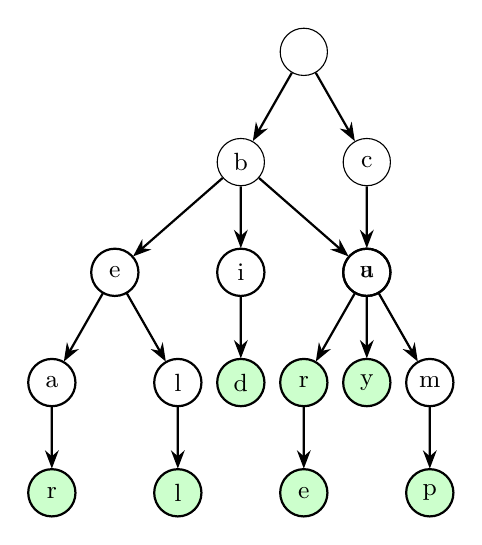
\begin{tikzpicture}[
    every node/.style={circle, draw, minimum size=6mm, inner sep=1pt,
                       font=\small},
    edge from parent/.style={draw, -{Stealth}, thick},
    level distance=14mm, sibling distance=16mm
  ]
  \node (root) {\phantom{x}}
    child { node (b) {b}
      child { node (e) {e}
        child { node (a) {a}
          child { node[fill=green!20] (r1) {r} }
        }
        child { node (l1) {l}
          child { node[fill=green!20] (l2) {l} }
        }
      }
      child { node (i) {i}
        child { node[fill=green!20] (d) {d} }
      }
      child { node (u) {u}
        child { node[fill=green!20] (y) {y} }
      }
    }
    child { node (c) {c}
      child { node (a2) {a}
        child { node[fill=green!20] (r2) {r}
          child { node[fill=green!20] (e2) {e} }
        }
        child { node (m) {m}
          child { node[fill=green!20] (p) {p} }
        }
      }
    };
\end{tikzpicture}%
}
\caption{Trie storing seven strings. Green-shaded nodes have
         \texttt{is\_end\_of\_word = True}.}
\label{fig:trie-example}
\end{figure}

% -----------------------------------------------------------------------
\section{Applications of Tries}
\label{sec:trie-applications}

Tries appear in a wide range of practical systems:

\begin{itemize}
  \item \textbf{Autocomplete.} Search engines and mobile keyboards use tries
        to suggest completions as the user types, because prefix lookup is
        proportional only to the length of the typed prefix.
  \item \textbf{Spell checking.} A dictionary stored as a trie allows $O(L)$
        verification of whether a word exists, and can generate corrections
        using prefix matching or edit-distance techniques.
  \item \textbf{IP routing.} Longest-prefix matching in routing tables is
        naturally expressed as a trie traversal on binary representations of
        IP addresses.
  \item \textbf{Compression.} Algorithms such as LZW leverage trie-based
        pattern recognition to compress data.
\end{itemize}

% -----------------------------------------------------------------------
\section{Trie Implementation Strategies}
\label{sec:trie-impl}

Each internal node of a trie must map a character to a child node.  Three
common representations exist for this mapping.

\subsection{Hash Table Children}
\label{subsec:trie-hash}

Each node stores a Python dictionary \texttt{children} keyed by character.
Lookup and insertion at each node are $O(1)$ average-case.

\begin{lstlisting}[language=Python]
class TrieNode:
    def __init__(self):
        self.children = {}
        self.is_end_of_word = False
\end{lstlisting}

\subsection{Array Children}
\label{subsec:trie-array}

Each node stores a fixed-size array of length $|\Sigma|$ (e.g.\ 26 for
lowercase English letters).  Access is $O(1)$ worst-case, but the space cost
is $O(|\Sigma|)$ per node regardless of how many children actually exist.

\begin{lstlisting}[language=Python]
class TrieNode:
    def __init__(self):
        self.children = [None] * 26
        self.is_end_of_word = False
\end{lstlisting}

\subsection{Linked List Children (Left-Child Right-Sibling)}
\label{subsec:trie-ll}

Each node stores a single character, a pointer to its \emph{first child},
and a pointer to the \emph{next sibling} at the same level.  This is the
classic left-child right-sibling (LCRS) representation and is the primary
implementation studied in this course.

\begin{definition}[Trie Node (Linked-List Representation)]
\label{def:trie-node-ll}
A \texttt{TrieNode} consists of four fields:
\begin{enumerate}
  \item \texttt{char} --- the character stored at this node,
  \item \texttt{is\_end\_of\_word} --- boolean flag indicating whether this
        node completes a stored string,
  \item \texttt{child} --- pointer to the first child node (one level deeper
        in the trie), and
  \item \texttt{next} --- pointer to the next sibling node (same depth,
        same parent).
\end{enumerate}
\end{definition}

\begin{lstlisting}[language=Python]
class TrieNode:
    def __init__(self, char):
        self.char = char
        self.is_end_of_word = False
        self.child = None
        self.next = None
\end{lstlisting}

The \texttt{Trie} class itself holds a reference to a dummy root node:

\begin{lstlisting}[language=Python]
class Trie:
    def __init__(self):
        self.root = TrieNode("")
\end{lstlisting}

\begin{examtip}[title={Exam Tip: Navigating the Linked-List Trie}]
In the LCRS representation, \texttt{child} moves \emph{down} a level
(to the children of a node), while \texttt{next} moves \emph{across}
siblings at the same level.  Searching for a particular character among a
node's children requires traversing the sibling chain via \texttt{next},
which takes $O(|\Sigma|)$ in the worst case.
\end{examtip}

% -----------------------------------------------------------------------
\section{Core Operations}
\label{sec:trie-ops}

The linked-list trie supports three primary operations: searching for a word,
inserting a word, and traversal.  Deletion is rarely implemented in practice
because dictionaries seldom change and deletion logic is substantially more
complex than insertion.

\subsection{Helper: Finding a Child}
\label{subsec:trie-find-child}

Both search and insert rely on a helper that traverses the sibling linked list
of a node's children to locate a given character.

\begin{lstlisting}[language=Python]
def _find_child(self, node, char):
    current = node.child
    while current:
        if current.char == char:
            return current
        current = current.next
    return None
\end{lstlisting}

The helper returns the matching \texttt{TrieNode} if found, or \texttt{None}
otherwise.  Its time complexity is $O(k)$ where $k$ is the number of children
of \texttt{node} (at most $|\Sigma|$).

\subsection{Searching for a Word}
\label{subsec:trie-search}

To search for a word, we walk down from the root, consuming one character per
level.  If at any level the character is absent among the current node's
children, the word is not in the trie.  If we reach the end of the word, we
check \texttt{is\_end\_of\_word} to distinguish stored words from mere
prefixes.

\begin{lstlisting}[language=Python]
def search(self, word):
    node = self.root
    for char in word:
        node = self._find_child(node, char)
        if not node:
            return False
    return node.is_end_of_word
\end{lstlisting}

\begin{example}[Searching for ``bell'']
\label{ex:trie-search-bell}
Starting from the root: find \texttt{`b'} among root's children $\to$
found; find \texttt{`e'} among \texttt{b}'s children $\to$ found; find
\texttt{`l'} among \texttt{e}'s children $\to$ found; find \texttt{`l'}
among the first \texttt{l}'s children $\to$ found.  The final node has
\texttt{is\_end\_of\_word = True}, so the search returns \texttt{True}.

Searching for \texttt{``bel''} would follow the same path but stop one level
earlier, where \texttt{is\_end\_of\_word = False}, so it returns
\texttt{False}---the string is a prefix of a stored word but is not itself
stored.
\end{example}

\subsection{Inserting a Word}
\label{subsec:trie-insert}

Insertion walks the same path as search, but creates new nodes for any
character not yet present.  New children are inserted \emph{at the head} of
the sibling linked list for $O(1)$ insertion.

\begin{lstlisting}[language=Python]
def _add_child(self, node, char):
    new_node = TrieNode(char)
    new_node.next = node.child
    node.child = new_node
    return new_node

def insert(self, word):
    node = self.root
    for char in word:
        child = self._find_child(node, char)
        if not child:
            child = self._add_child(node, char)
        node = child
    node.is_end_of_word = True
\end{lstlisting}

After processing every character, the last visited node is marked as an
end-of-word.  If the word (or a prefix of it) already exists, the algorithm
simply walks existing nodes and sets the flag at the end.

\begin{warning}[title={Warning: Insertion Order Affects Sibling Order}]
Because \texttt{\_add\_child} prepends to the sibling list, the order of
children at any node depends on the order in which words were inserted.  A
DFS traversal will therefore enumerate words in an order that reflects
insertion history, not necessarily alphabetical order.
\end{warning}

% -----------------------------------------------------------------------
\section{Trie Traversal}
\label{sec:trie-traversal}

The binary tree traversal paradigms from Chapter~\ref{ch:binary-trees}
generalise naturally to tries.  Since a trie node may have an arbitrary
number of children (linked via \texttt{child}/\texttt{next}), we iterate over
the sibling chain rather than visiting fixed left and right pointers.

\subsection{Depth-First Search (Preorder)}
\label{subsec:trie-dfs}

Preorder DFS visits a node before recursing into its children.  For each
child, we recurse, then advance to the next sibling.

\begin{lstlisting}[language=Python]
def dfs(self, node):
    if node is not None:
        print(node.char, end=" ")
        child = node.child
        while child:
            self.dfs(child)
            child = child.next
\end{lstlisting}

For the trie in Figure~\ref{fig:trie-example}, calling
\texttt{dfs(root)} produces the traversal order:
\begin{multline*}
  \texttt{root} \;\to\; b \;\to\; e \;\to\; a \;\to\; r \;\to\;
  l \;\to\; l \;\to\; i \;\to\; d \;\to\; u \;\to\; y \\
  \to\; c \;\to\; a \;\to\; r \;\to\; e \;\to\; m \;\to\; p.
\end{multline*}

\subsection{Breadth-First Search (Level-by-Level)}
\label{subsec:trie-bfs}

BFS uses a queue (cf.\ Chapter~\ref{ch:queues}) to visit nodes level by level.
When a node is dequeued, all its children are enqueued via the sibling chain.

\begin{lstlisting}[language=Python]
def bfs(self):
    queue = Queue()
    queue.enqueue(self.root)
    while not queue.is_empty():
        node = queue.dequeue()
        print(node.char, end=" ")
        child = node.child
        while child:
            queue.enqueue(child)
            child = child.next
\end{lstlisting}

The BFS order for Figure~\ref{fig:trie-example} is:
\begin{multline*}
  \texttt{root} \;\to\; b \;\to\; c \;\to\; e \;\to\; i \;\to\;
  u \;\to\; a \;\to\; a \;\to\; l \;\to\; d \;\to\; y \\
  \to\; r \;\to\; m \;\to\; r \;\to\; l \;\to\; e \;\to\; p.
\end{multline*}

% -----------------------------------------------------------------------
\section{Application: Printing All Words}
\label{sec:trie-print-all}

A common task is to enumerate every word stored in a trie.  Both DFS and BFS
approaches carry a \texttt{prefix} string that accumulates characters along
the path from the root; whenever an end-of-word node is reached, the prefix
is a complete stored word.

\subsection{DFS Approach}
\label{subsec:trie-print-dfs}

\begin{lstlisting}[language=Python]
def print_all_words_dfs(self, node, prefix):
    if node.is_end_of_word:
        print(prefix)
    child = node.child
    while child:
        self.print_all_words_dfs(child,
            prefix + child.char)
        child = child.next
\end{lstlisting}

Calling \texttt{print\_all\_words\_dfs(root, "")} on the example trie prints
the words in depth-first order: \texttt{bear}, \texttt{bell}, \texttt{bid},
\texttt{buy}, \texttt{car}, \texttt{care}, \texttt{camp}.

\subsection{BFS Approach}
\label{subsec:trie-print-bfs}

In the BFS variant, the queue stores \emph{pairs} of (node, prefix).

\begin{lstlisting}[language=Python]
def print_all_words_bfs(self):
    queue = Queue()
    queue.enqueue((self.root, ""))
    while not queue.is_empty():
        node, prefix = queue.dequeue()
        if node.is_end_of_word:
            print(prefix)
        child = node.child
        while child:
            queue.enqueue((child,
                prefix + child.char))
            child = child.next
\end{lstlisting}

\begin{keyresult}[title={Key Result: Trie Traversal Complexity}]
Both DFS and BFS visit every node in the trie exactly once.  If the trie
contains $N$ nodes, traversal is $O(N)$.  Printing all words additionally
incurs $O(L)$ per word for string concatenation, where $L$ is the word's
length.
\end{keyresult}

% -----------------------------------------------------------------------
\section{Application: Autocomplete}
\label{sec:trie-autocomplete}

Autocomplete suggests possible completions for a given prefix.  The algorithm
has two phases:

\begin{enumerate}
  \item \textbf{Navigate to the prefix node.}  Starting from the root, follow
        edges matching each character of the prefix using
        \texttt{\_find\_child}.  If the prefix is not present in the trie,
        there are no suggestions.
  \item \textbf{Collect all words below.}  From the prefix node, perform a
        DFS or BFS (as in Section~\ref{sec:trie-print-all}) to enumerate
        every stored word that extends the prefix.
\end{enumerate}

For instance, searching for the prefix \texttt{``ca''} in the example trie
navigates root $\to$ \texttt{c} $\to$ \texttt{a}, then collects the
completions \texttt{car}, \texttt{care}, and \texttt{camp}.  In practice,
results may be ranked by frequency, recency, or other heuristics before
being displayed to the user.

% -----------------------------------------------------------------------
\section{Application: Spell Checking}
\label{sec:trie-spellcheck}

A trie-based spell checker operates in two stages:

\begin{enumerate}
  \item \textbf{Validity check.}  Search the trie for the input word.  If
        \texttt{search} returns \texttt{True}, the word is valid.
  \item \textbf{Suggestion generation.}  If the word is invalid, generate
        candidate corrections.  Common strategies include:
        \begin{itemize}
          \item \emph{Prefix matching}---find stored words sharing the longest
                common prefix with the misspelled word.
          \item \emph{Edit distance}---use metrics such as Levenshtein distance
                to find words within a small number of insertions, deletions,
                or substitutions.
          \item \emph{Frequency ranking}---prioritise more commonly used words
                among the candidates.
          \item \emph{User history / context}---adjust rankings based on the
                user's prior input.
        \end{itemize}
\end{enumerate}

% -----------------------------------------------------------------------
\section{Summary}
\label{sec:trie-summary}

\begin{keyresult}[title={Key Result: Trie Operations}]
\begin{enumerate}
  \item A \textbf{trie} stores a set of strings by sharing common prefixes,
        achieving $O(L)$ search and insertion for a string of length~$L$.
  \item The \textbf{linked-list (LCRS) representation} uses \texttt{child}
        and \texttt{next} pointers; finding a child costs $O(|\Sigma|)$ per
        level in the worst case.
  \item \textbf{DFS} (preorder) and \textbf{BFS} (level-by-level) both visit
        every node once in $O(N)$ time and extend naturally from binary tree
        traversals to the multi-child trie setting.
  \item \textbf{Autocomplete} navigates to a prefix node, then collects all
        words below via traversal.
  \item \textbf{Spell checking} combines trie search with edit-distance or
        prefix-matching heuristics to suggest corrections.
\end{enumerate}
\end{keyresult}

\chapter{Heaps}
\label{ch:heaps}

A \emph{heap} is a specialised binary tree that maintains a simple ordering invariant between parents and children.  Because heaps can be stored compactly in a contiguous array with no pointers, they underpin several fundamental data-structure and algorithm-design patterns, including priority queues (introduced informally in Chapter~\ref{ch:pq-apps}) and an efficient $O(n\log n)$ sorting algorithm.

%----------------------------------------------------------------------
\section{Definition and Properties}
\label{sec:heap-def}

\begin{definition}[Binary Heap]
\label{def:binary-heap}
A \textbf{binary heap} is a complete binary tree satisfying the \emph{heap-order property}.  A binary tree is \emph{complete} when every level is fully occupied except possibly the last, which is filled from left to right.  Two variants exist:
\begin{itemize}
  \item \textbf{Max-heap}: for every node~$i$ (other than the root), $A[\operatorname{parent}(i)] \ge A[i]$.
  \item \textbf{Min-heap}: for every node~$i$ (other than the root), $A[\operatorname{parent}(i)] \le A[i]$.
\end{itemize}
\end{definition}

In a max-heap the largest element is always at the root; in a min-heap the smallest element is at the root.  Neither variant imposes any ordering between siblings---only the parent--child relationship matters.

\begin{examtip}[title={Exam Tip: Heap vs.\ BST}]
A heap is \emph{not} a binary search tree.  In a BST the left child is smaller and the right child is larger; in a heap both children are smaller (max-heap) or both are larger (min-heap).  No left--right ordering is guaranteed.
\end{examtip}

%----------------------------------------------------------------------
\section{Array Representation}
\label{sec:heap-array}

Because a heap is a \emph{complete} binary tree, it can be stored in a simple array with no explicit child or parent pointers.  For the node at index~$i$ (0-indexed):
\begin{align}
  \operatorname{left}(i)   &= 2i + 1, \label{eq:heap-left}\\
  \operatorname{right}(i)  &= 2i + 2, \label{eq:heap-right}\\
  \operatorname{parent}(i) &= \left\lfloor \frac{i-1}{2} \right\rfloor. \label{eq:heap-parent}
\end{align}

The height of a heap with $n$ elements is $\lfloor \log_2 n \rfloor$, which bounds the cost of any root-to-leaf traversal.

\begin{example}[Max-Heap Array Layout]
\label{ex:heap-array}
Consider the max-heap $[25,\,20,\,16,\,9,\,8,\,5,\,2]$.  The root is $A[0]=25$; its children are $A[1]=20$ and $A[2]=16$.  The children of $A[1]=20$ are $A[3]=9$ and $A[4]=8$, while those of $A[2]=16$ are $A[5]=5$ and $A[6]=2$.  Every parent is at least as large as its children, confirming the max-heap property.
\end{example}

\begin{figure}[h]
\centering
\resizebox{\linewidth}{!}{%
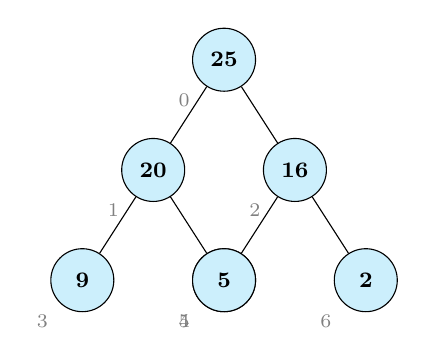
\begin{tikzpicture}[
    node/.style={draw, circle, minimum size=8mm, font=\footnotesize\bfseries, fill=cyan!20},
    idx/.style={font=\scriptsize\color{gray}},
    arr/.style={-{Stealth}, thick},
    level distance=14mm,
    sibling distance=18mm,
  ]
  \node[node] (n0) {25}
    child { node[node] (n1) {20}
      child { node[node] (n3) {9} }
      child { node[node] (n4) {8} }
    }
    child { node[node] (n2) {16}
      child { node[node] (n5) {5} }
      child { node[node] (n6) {2} }
    };
  \node[idx, below left=1pt of n0] {0};
  \node[idx, below left=1pt of n1] {1};
  \node[idx, below left=1pt of n2] {2};
  \node[idx, below left=1pt of n3] {3};
  \node[idx, below left=1pt of n4] {4};
  \node[idx, below left=1pt of n5] {5};
  \node[idx, below left=1pt of n6] {6};
\end{tikzpicture}%
}
\caption{A max-heap of seven elements and its array representation
         $[\,25,\;20,\;16,\;9,\;8,\;5,\;2\,]$.}
\label{fig:max-heap}
\end{figure}

\begin{keyresult}[title={Key Result: Heap Index Formulas}]
For a 0-indexed array, the children of node~$i$ are at $2i+1$ and $2i+2$;
its parent is at $\lfloor(i-1)/2\rfloor$.  The height of an $n$-element heap
is $\lfloor\log_2 n\rfloor$.
\end{keyresult}

%----------------------------------------------------------------------
\section{Core Operations}
\label{sec:heap-ops}

\subsection{Heapify (Sift Down)}
\label{subsec:heapify}

The \textsc{Max-Heapify} procedure restores the max-heap property at a single node~$i$, assuming that the subtrees rooted at the left and right children of~$i$ are already valid max-heaps.  It compares $A[i]$ with its two children, swaps $A[i]$ with the largest child if necessary, and recurses on the affected subtree.

\begin{algorithm}[h]
\caption{\textsc{Max-Heapify}$(A, i)$}
\label{alg:max-heapify}
\begin{algorithmic}[1]
\State $l \gets \operatorname{left}(i)$
\State $r \gets \operatorname{right}(i)$
\If{$l < \text{size}(A)$ \textbf{and} $A[l] > A[i]$}
    \State $\text{largest} \gets l$
\Else
    \State $\text{largest} \gets i$
\EndIf
\If{$r < \text{size}(A)$ \textbf{and} $A[r] > A[\text{largest}]$}
    \State $\text{largest} \gets r$
\EndIf
\If{$\text{largest} \neq i$}
    \State exchange $A[i]$ and $A[\text{largest}]$
    \State \textsc{Max-Heapify}$(A, \text{largest})$
\EndIf
\end{algorithmic}
\end{algorithm}

\begin{example}[Heapify Trace]
\label{ex:heapify-trace}
Starting with the array $[\,16,\,4,\,10,\,14,\,7,\,9,\,3,\,2,\,8,\,1\,]$, calling \textsc{Max-Heapify}$(A,1)$ proceeds as follows.  Node~1 holds~4, whose children are $A[3]=14$ and $A[4]=7$.  Since $14>4$, we swap 4~and~14, giving $[\,16,\,14,\,10,\,4,\,7,\,9,\,3,\,2,\,8,\,1\,]$.  Now node~3 holds~4 with children $A[7]=2$ and $A[8]=8$.  Since $8>4$, we swap 4~and~8, yielding the final array $[\,16,\,14,\,10,\,8,\,7,\,9,\,3,\,2,\,4,\,1\,]$.  The subtree rooted at index~1 is now a valid max-heap.
\end{example}

The element ``floats down'' at most $h=\lfloor\log_2 n\rfloor$ levels, performing $O(1)$ work per level, so the running time is $O(\log n)$.

\subsection{Build Heap}
\label{subsec:build-heap}

To convert an arbitrary array of $n$ elements into a max-heap, we apply \textsc{Max-Heapify} to every non-leaf node, working from the last internal node up to the root.  Leaf nodes (indices $\lfloor n/2\rfloor$ through $n-1$) are trivially valid one-element heaps.

\begin{algorithm}[h]
\caption{\textsc{Build-Max-Heap}$(A)$}
\label{alg:build-heap}
\begin{algorithmic}[1]
\For{$i = \lfloor(\text{length}(A)-1)/2\rfloor$ \textbf{down to} $0$}
    \State \textsc{Max-Heapify}$(A, i)$
\EndFor
\end{algorithmic}
\end{algorithm}

\begin{example}[Building a Max-Heap]
\label{ex:build-heap}
Given $A = [\,4,\,1,\,3,\,2,\,16,\,9,\,10,\,14,\,8,\,7\,]$, the last internal node is at index~$\lfloor(10-1)/2\rfloor = 4$.  Heapifying from index~4 down to~0 proceeds through the following key snapshots:
\begin{enumerate}
  \item Index~4 ($A[4]=16$): children are $A[9]=7$; already valid---no swap.
  \item Index~3 ($A[3]=2$): child $A[7]=14$ is larger; swap $\Rightarrow A[3]=14$.
  \item Index~2 ($A[2]=3$): child $A[6]=10$ is larger; swap $\Rightarrow A[2]=10$.
  \item Index~1 ($A[1]=1$): child $A[3]=14$ is larger; swap, then recurse.
  \item Index~0 ($A[0]=4$): child $A[1]=16$ is larger; swap, then recurse.
\end{enumerate}
The final max-heap is $[\,16,\,14,\,10,\,8,\,7,\,9,\,3,\,2,\,4,\,1\,]$.
\end{example}

\begin{keyresult}[title={Key Result: Build-Heap is $O(n)$}]
Although there are $O(n)$ calls to \textsc{Max-Heapify}, each costing $O(\log n)$ in the worst case, a tighter analysis shows that most nodes are near the bottom of the tree and heapify over very few levels.  Summing across all levels gives a total cost of $O(n)$, \emph{not} $O(n\log n)$.
\end{keyresult}

\subsection{Insertion}
\label{subsec:heap-insert}

To insert a new key into a max-heap:
\begin{enumerate}
  \item Place the new element at the next available position (the end of the array), preserving the complete-tree shape.
  \item \textbf{Bubble up}: repeatedly compare the new element with its parent and swap if the new element is larger, until the heap-order property is restored or the root is reached.
\end{enumerate}

The new element rises at most $h$ levels, so insertion runs in $O(\log n)$.

\begin{example}[Inserting 15 into a Max-Heap]
\label{ex:heap-insert}
Starting from the max-heap $[\,16,\,14,\,10,\,8,\,7,\,9,\,3,\,2,\,4,\,1\,]$, we append 15~at index~10.  Since $15 > A[\operatorname{parent}(10)] = A[4] = 7$, swap to get $A[4]=15$.  Then $15 > A[\operatorname{parent}(4)] = A[1] = 14$, swap to get $A[1]=15$.  Finally $15 < A[0] = 16$, so the process stops.  The resulting heap is $[\,16,\,15,\,10,\,8,\,14,\,9,\,3,\,2,\,4,\,1,\,7\,]$.
\end{example}

\subsection{Deletion}
\label{subsec:heap-delete}

To delete an arbitrary node at index~$i$ from a max-heap:
\begin{enumerate}
  \item Replace $A[i]$ with the last element of the heap.
  \item Remove the last element (decrease heap size by one).
  \item Restore the heap property:
  \begin{itemize}
    \item If the replacement value is \emph{greater} than its parent, \textbf{bubble up}.
    \item If it is \emph{smaller} than one of its children, \textbf{heapify down}.
  \end{itemize}
\end{enumerate}

Since either direction traverses at most $O(\log n)$ levels, deletion runs in $O(\log n)$.

\begin{example}[Deleting the Root (Extract-Max)]
\label{ex:heap-delete}
From $[\,16,\,15,\,10,\,8,\,14,\,9,\,3,\,2,\,4,\,1,\,7\,]$, delete the root ($16$).  Replace $A[0]$ with the last element~$7$, giving $[\,7,\,15,\,10,\,8,\,14,\,9,\,3,\,2,\,4,\,1\,]$.  Now heapify down from index~0: swap $7$~with~$15$ (index~1), then swap $7$~with~$14$ (index~4).  The resulting heap is $[\,15,\,14,\,10,\,8,\,7,\,9,\,3,\,2,\,4,\,1\,]$.
\end{example}

\begin{warning}[title={Common Mistake: Forgetting to Check Both Directions}]
When deleting a node that is not the root, the replacement value could be either larger or smaller than its new neighbours.  Always check \emph{both} the parent (for a possible bubble up) \emph{and} the children (for a possible heapify down).  Checking only one direction leaves the heap in an invalid state.
\end{warning}

%----------------------------------------------------------------------
\section{Complexity Summary}
\label{sec:heap-complexity}

\begin{center}
\begin{tabular}{lcc}
\toprule
\textbf{Operation} & \textbf{Time} & \textbf{Notes} \\
\midrule
Build Heap       & $O(n)$       & Bottom-up construction \\
Insert           & $O(\log n)$  & Bubble up \\
Delete           & $O(\log n)$  & Replace + heapify/bubble \\
Heapify          & $O(\log n)$  & Sift down one path \\
Find max / min   & $O(1)$       & Root of max-/min-heap \\
\bottomrule
\end{tabular}
\end{center}

%----------------------------------------------------------------------
\section{Applications}
\label{sec:heap-apps}

Heaps underlie several important algorithms and data-structure patterns:

\begin{enumerate}
  \item \textbf{Priority queues.}  A max- or min-heap provides $O(\log n)$ insertion and $O(\log n)$ extract-max/min, making it the standard implementation of a priority queue.  Operating-system task schedulers and print queues are classic examples.

  \item \textbf{Heap sort.}  Build a max-heap from the input array ($O(n)$), then repeatedly extract the maximum and place it at the end of the array.  Each extraction costs $O(\log n)$, giving an overall time complexity of $O(n\log n)$ with $O(1)$ extra space.

  \item \textbf{Graph algorithms.}
  \begin{itemize}
    \item \emph{Dijkstra's algorithm} uses a min-heap (priority queue) to repeatedly select the unvisited vertex with the smallest tentative distance, achieving $O((V+E)\log V)$.
    \item \emph{Prim's algorithm} uses a min-heap to pick the cheapest edge crossing the cut at each step when building a minimum spanning tree.
  \end{itemize}
\end{enumerate}

%----------------------------------------------------------------------
\section{Summary}
\label{sec:heap-summary}

\begin{keyresult}[title={Key Result: Heap Operations}]
\begin{enumerate}
  \item A \textbf{binary heap} is a complete binary tree stored in an array; the parent--child
        relationship is computed via index arithmetic ($2i+1$, $2i+2$, $\lfloor(i-1)/2\rfloor$).
  \item \textsc{Max-Heapify} restores the heap property at a single node in $O(\log n)$ by
        sifting down; \textsc{Build-Max-Heap} converts an arbitrary array in $O(n)$.
  \item Insertion (bubble up) and deletion (replace + heapify/bubble) both run in $O(\log n)$.
  \item Heaps are the standard backing structure for priority queues and enable heap sort
        ($O(n\log n)$, in-place) and efficient graph algorithms (Dijkstra, Prim).
\end{enumerate}
\end{keyresult}

\end{document}
